\documentclass{workbook}

\newcommand{\copyrightdate}{\the\year}

\usepackage{ifxetex}
\usepackage[utf8]{inputenc}
\usepackage{hyperref}
\usepackage{hyperxmp} % Embed meta data into the PDF
\hypersetup{%
	hidelinks=true,
	linkcolor = {0 0 1},
	% Metadata to be embedded by hyperxmp
	pdftitle={Mathematical Modelling (\jobname)},
	pdfauthor={Bernardo Galv\~ao-Sousa},
	pdfauthortitle={Author},
	pdfcopyright={Copyright (C) \copyrightdate, Bernardo Galv\~ao-Sousa},
	pdfsubject={Mathematical Modelling textbook/workbook},
	pdfkeywords={modeling, modelling, vectors, mathematics, textbook, ODEs, PDEs, optimization},
	pdfurl={https://github.com/bigfatbernie/IBLMathModeling/},
	pdflicenseurl={https://creativecommons.org/licenses/by-sa/4.0/},
}

\usepackage{multirow}
\usetikzlibrary{arrows,snakes,backgrounds,patterns,shapes.geometric,calc,automata, positioning}


%%%
% import all needed packages and macros
%%%
\usepackage[yyyymmdd]{datetime}
%%
%% All packages and macros needed for the problemsets
%%

\usepackage{amsmath}

\usepackage{lipsum}
%\usepackage{showframe}
%\usepackage{layout}


\usepackage[charter,cal=cmcal]{mathdesign} %different font
%\usepackage{avant}

\usepackage{microtype}
\usepackage{mathtools}
\usepackage{etoolbox}
%\usepackage{amsfonts}
%\usepackage{amssymb}
\usepackage{graphicx}
\graphicspath{{images/}}
\usepackage[inline]{enumitem}
\usepackage{xparse}
\usepackage{ifthen}
\usepackage{caption}
\usepackage{subcaption}
\usepackage{tikz}
	\usetikzlibrary{fit}
	\usetikzlibrary{fadings}
	\usetikzlibrary{calc}
	\tikzset{>=latex}
	\usetikzlibrary{cd}
	\usetikzlibrary{spy}
	\usetikzlibrary{patterns}
	\usetikzlibrary{decorations, decorations.pathreplacing, decorations.markings}

\usepackage{fancyhdr}
\usepackage{calc}
\usepackage{wrapfig}
\usepackage{marginnote}
\usepackage{mparhack}
\usepackage{marginfix}
\usepackage{indextools}
\usepackage[open=false]{bookmark}  % render the pdf TOC in the proper order
\hypersetup{
	hidelinks=true,
	linkcolor = {0 0 1},
	unicode=true,
	psdextra=true,
}
\usepackage{common/nicematrix}

%\usepackage[
%  linktocpage=false,      % no page numbers are clickable
%  colorlinks=false,       % no color
%  breaklinks=true,        % break URLs
%  bookmarks,              % creates bookmarks in pdf
%  hyperfootnotes=true,    % clickable footnotes
%  pdfborder={0 0 0},      % for removing borders around links
%  bookmarksnumbered=true, % If Acrobat bookmarks are requested, include section numbers.
%  bookmarksopen=false,    % If Acrobat bookmarks are requested, show them with all the subtrees expanded.
%  %hidelinks=true,
%  %linkcolor=blue,
%  %citecolor=blue,
%  %urlcolor=blue,
%  pdfpagemode={UseOutlines}, % show pdf bookmarks (indices) on startup; does not function all the time
%  pdftitle={...}, % title
%  pdfauthor={...}, % author
%  pdfkeywords={...}, % subject of the document
%  pdfsubject={...}, % list of keywords
%  pdfmenubar=true,        % make PDF viewer’s menu bar visible
%  pdfpagelabels,
%]{hyperref}
%\usepackage[hidelinks,]{hyperref}
\usepackage{fnpct} % fancy footnote spacing
\usepackage{bm}
\usepackage{systeme}
\usepackage{datatool}% http://ctan.org/pkg/datatool for sorted lists
\usepackage{xspace}


\usepackage{pgfplots}
\pgfplotsset{compat=1.16}
	\usepgfplotslibrary{fillbetween}
%%%
% Useful Linear Algebra macros
%%%
\newcommand{\declarecommand}[1]{\providecommand{#1}{}\renewcommand{#1}}
\DeclareDocumentCommand{\R}{}{\mathbb{R}}  % we don't care if it's already defined.  We really want *this* command!
\DeclareDocumentCommand{\Z}{}{\mathbb{Z}}
\DeclareDocumentCommand{\Q}{}{\mathbb{Q}}
\DeclareDocumentCommand{\N}{}{\mathbb{N}}
\DeclareDocumentCommand{\C}{}{\mathbb{C}}
\DeclareDocumentCommand{\d}{}{\mathrm{d}}
\DeclareDocumentCommand{\dd}{}{\mathbbm{d}} % exterior derivative
\DeclareMathOperator{\Span}{span}
\DeclareMathOperator{\Img}{img}
\DeclareMathOperator{\Id}{id}
\DeclareMathOperator{\Ident}{\Id}
\DeclareMathOperator{\Vol}{Vol}
\DeclareMathOperator{\VolChange}{Vol\hspace{1.5pt}Change}
\DeclareMathOperator{\Range}{range}
\DeclareMathOperator{\Rref}{rref}
\DeclareMathOperator{\Rank}{rank}
\DeclareMathOperator{\Comp}{\Vcomp}
\DeclareMathOperator{\Vcomp}{v\hspace{1pt}comp}
\DeclareMathOperator{\Null}{null}
\DeclareMathOperator{\Nullity}{nullity}
\DeclareMathOperator{\Char}{char}
\DeclareMathOperator{\Proj}{proj}
\DeclareMathOperator{\Flux}{Flux}
\DeclareMathOperator{\Circ}{Circ}
\DeclareMathOperator{\chr}{char}
\DeclareMathOperator{\Dim}{dim}
\DeclareMathOperator{\Perp}{perp}
\DeclareMathOperator{\Ker}{kernel}
\DeclareMathOperator{\Row}{row}
\DeclareMathOperator{\Col}{col}
\DeclareMathOperator{\Rep}{Rep}
\newcommand{\BasisChange}[2]{[#2\!\leftarrow\!#1]}
\newcommand{\proj}{\Proj}
\newcommand{\rref}{\Rref}
\newcommand{\xhat}{{\vec e_1}}
\newcommand{\yhat}{{\vec e_2}}
\newcommand{\zhat}{{\vec e_3}}
\newcommand{\sbasis}[1]{\vec { e}_{#1}}
\newcommand{\mat}[1]{\begin{bmatrix*}[r]#1\end{bmatrix*}}
\newcommand{\matp}[1]{\begin{pmatrix*}[r]#1\end{pmatrix*}}
\newcommand{\matc}[1]{\begin{bmatrix}#1\end{bmatrix}}
\newcommand{\matpc}[1]{\begin{pmatrix}#1\end{pmatrix}}
\newcommand{\formarg}[2]{\big(#1;\, #2\big)}
\DeclarePairedDelimiter\abs{\lvert}{\rvert}
\DeclarePairedDelimiter\Abs{\lvert}{\rvert}
\DeclarePairedDelimiter\norm{\lVert}{\rVert}
\newcommand{\Norm}[1]{\norm{#1}}
% just to make sure it exists
\providecommand\given{}
% can be useful to refer to this outside \Set
\newcommand\SetSymbol[1][]{%
	\nonscript\::%
	\allowbreak
	\nonscript\:
	\mathopen{}}
\DeclarePairedDelimiterX\Set[1]\{\}{%
	\renewcommand\given{\SetSymbol[\delimsize]}
	#1
}
\newcommand{\Rrefto}{\xrightarrow{\text{row reduces to}}}


% redefine bmatrix,etc to allow optional argument for augmenting
% code from https://tex.stackexchange.com/questions/2233/whats-the-best-way-make-an-augmented-coefficient-matrix
\makeatletter
\renewcommand*\env@matrix[1][*\c@MaxMatrixCols c]{%
  \hskip -\arraycolsep
  \let\@ifnextchar\new@ifnextchar
  \array{#1}}
\makeatother

\newcommand{\scaledgrid}[1]{%
	\begin{tikzpicture}[scale=#1]
		\draw[thin, white!20!black, dotted] (-4.1,-4.1) grid (4.1,4.1);
		\draw[ <->] (-4.3,0) -- (4.3,0);
		\draw[ <->] (0,-4.3) -- (0,4.3);
	\end{tikzpicture}
}
\newcommand{\scaledshortgrid}[1]{%
	\begin{tikzpicture}[scale=#1]
		\draw[thin, white!20!black, dotted] (-4.1,-2.1) grid (4.1,2.1);
		\draw[ <->] (-4.3,0) -- (4.3,0);
		\draw[ <->] (0,-2.3) -- (0,2.3);
	\end{tikzpicture}
}
\newcommand{\singlegrid}{\scaledgrid{1}}
\newcommand{\doublegrid}{\mbox{\scaledgrid{.9}\scaledgrid{.9}}\par}
\newcommand{\triplegrid}{\mbox{\scaledgrid{.6}\scaledgrid{.6}\scaledgrid{.6}}\par}

% labels for source attributions
\NewDocumentCommand{\beezer}{o}{%
	\IfNoValueTF{#1}{%
		{\color{blue}\sffamily{B}}%
	}{%
		{\color{blue}\sffamily{B}}%  XXX Todo, make this href to the appropriate problem number
	}\xspace%
}
\NewDocumentCommand{\hefferon}{o}{%
	\IfNoValueTF{#1}{%
		{\color{blue}\sffamily{H}}%
	}{%
		{\color{blue}\sffamily{H}}%  XXX Todo, make this href to the appropriate problem number
	}\xspace%
}

\DeclareDocumentEnvironment{beforeyouread}{}{
Before you read, make sure you are comfortable with the following.
Please do the ``Quick Check'' problem to see if you are comfortable with each
task.
\begin{itemize}
}{
\end{itemize}
}
\newcommand\quickcheck[1]{\par {\footnotesize \textsc{Quick Check.} \textrm{#1}}}

% Dummy, voidable environments
\DeclareDocumentEnvironment{bookonly}{o}{}{}
\DeclareDocumentEnvironment{displayonly}{o}{}{}
\DeclareDocumentEnvironment{slidesonly}{o}{}{}
\DeclareDocumentEnvironment{bigcover}{o}{}{}

\newcommand{\hdash}{\text{\-------}}
\newcommand{\bigmathstrut}{\vphantom{\Big(}}


\usepackage{breqn}
\usepackage{multirow, multicol}


\usepackage{pdfrender} % For text title

\usepackage[ruled,vlined, boxed]{algorithm2e} % For algorithm explanation


%%%
% Set up the footers to have the correct copyright notices
%%%

\fancypagestyle{siefken}{%
	\rfoot{\footnotesize\it \copyright\,Bernardo Galv\~ao-Sousa, \copyrightdate \ \makebox(30,5){
\includegraphics[height=1.2em]{by-sa.pdf}}}
	\lfoot{}
	\renewcommand{\headrulewidth}{0pt}
}


%%
% Allow hiding of environments
%%
\usepackage{environ}% http://ctan.org/pkg/environ
\makeatletter
\newcommand{\voidenvironment}[1]{%
  \expandafter\providecommand\csname env@#1@save@env\endcsname{}%
  \expandafter\providecommand\csname env@#1@process\endcsname{}%
  \@ifundefined{#1}{}{\RenewEnviron{#1}{}}%
}
\makeatother
% allow pagebreaks that only display in `standard` mode
\newcommand{\displayonlynewpage}{\begin{displayonly}\newpage\end{displayonly}}
% allow pagebreaks that only display in `book` mode
\newcommand{\bookonlynewpage}{\begin{bookonly}\newpage\end{bookonly}}


%
% Set up the three render modes: standard, instructor, and solutions.
% These render with varying amounts of extra data (like solutions and notes)
%
\newtoggle{instructor}
\newtoggle{standard}
\newtoggle{solutions}
\newtoggle{book}
\newtoggle{slides}
\newtoggle{slidessol}
\newtoggle{slideswhite}
\newcommand{\setinstructor}{
	\toggletrue{instructor}
	\togglefalse{standard}
	\togglefalse{solutions}
	\togglefalse{book}
	\togglefalse{slides}
	\togglefalse{slideswhite}
	\togglefalse{slidessol}
}
\newcommand{\setstandard}{
	\togglefalse{instructor}
	\toggletrue{standard}
	\togglefalse{solutions}
	\togglefalse{book}
	\togglefalse{slides}
	\togglefalse{slideswhite}
	\togglefalse{slidessol}
}
\newcommand{\setsolutions}{
	\togglefalse{instructor}
	\togglefalse{standard}
	\toggletrue{solutions}
	\togglefalse{book}
	\togglefalse{slides}
	\togglefalse{slideswhite}
	\togglefalse{slidessol}
}
\newcommand{\setbook}{
	\togglefalse{instructor}
	\togglefalse{standard}
	\togglefalse{solutions}
	\toggletrue{book}
	\togglefalse{slides}
	\togglefalse{slideswhite}
	\togglefalse{slidessol}
}
\newcommand{\setslides}{
	\togglefalse{instructor}
	\togglefalse{standard}
	\togglefalse{solutions}
	\togglefalse{book}
	\toggletrue{slides}
	\togglefalse{slideswhite}
	\togglefalse{slidessol}
}
\newcommand{\setslidessol}{
	\togglefalse{instructor}
	\togglefalse{standard}
	\togglefalse{solutions}
	\togglefalse{book}
	\togglefalse{slides}
	\togglefalse{slideswhite}
	\toggletrue{slidessol}
}
\newcommand{\setslideswhite}{
	\togglefalse{instructor}
	\togglefalse{standard}
	\togglefalse{solutions}
	\togglefalse{book}
	\togglefalse{slides}
	\toggletrue{slideswhite}
	\togglefalse{slidessol}
}


%
% Infer the document level from the \jobname
%
\usepackage{xstring}
\IfSubStr{\jobname}{\detokenize{book}}{\setbook}{
	\IfSubStr{\jobname}{\detokenize{solutions}}{\setsolutions}{
		\IfSubStr{\jobname}{\detokenize{slidessol}}{\setslidessol}{
			\IfSubStr{\jobname}{\detokenize{instructor}}{\setinstructor}{
				\IfSubStr{\jobname}{\detokenize{slides}}{\setslides}{
					\IfSubStr{\jobname}{\detokenize{white}}{\setslideswhite}{
							\setstandard
					}
				}
			}
		}
	}
}


\setbookoptions{
	twosided = false,
	inline solutions = false,
}


\NewColoredEnvironment{
	name = lesson,
	display name = Lesson,
	banner color = Plum,
	title color = Plum,
	banner on left = true,
	open right = false,
}
\NewColoredEnvironment{
	name = module,
	display name = Module,
	banner color = Turquoise,
	title color = Cerulean,
	definition color = Cerulean,
	theorem color = myorange,
}
\NewColoredEnvironment{
	name = appendix,
	display name = Appendix,
	banner color = LimeGreen,
	title color = LimeGreen!70!Green!80!black,
	definition color = Cerulean,
	theorem color = myorange,
}
\NewColoredEnvironment{
	name = indices,
	display name = Indices,
	banner color = Green,
	title color = Green,
}
\NewColoredEnvironment{
	name = tutorial,
	display name = Tutorial,
	banner color = Peach,
	title color = Peach!80!black,
	emphbox color = Peach,
	% We will print tutorial worksheets back-to-back to save space
	open right = false,
}




\loadgeometry{default}

%
% Hide the non-problem environments
%
\newcommand{\coversubtitle}{} % we override the subtitle in each mode, so make sure the command exists to override.
\iftoggle{instructor}{
	\voidenvironment{module}
	\voidenvironment{appendix}
	\voidenvironment{bookonly}
	\voidenvironment{slidesonly}
	\voidenvironment{displayonly}
	\renewcommand{\coversubtitle}{Instructor Guide}
}{}
\iftoggle{solutions}{
	\voidenvironment{module}
	\voidenvironment{appendix}
	\voidenvironment{bookonly}
	\voidenvironment{slidesonly}
	\voidenvironment{displayonly}
	\voidenvironment{lesson}
	\voidenvironment{notes}
	\renewcommand{\coversubtitle}{Solutions}
}{}
\iftoggle{standard}{
	\voidenvironment{module}
	\voidenvironment{appendix}
	\voidenvironment{bookonly}
	\voidenvironment{slidesonly}
	\voidenvironment{solution}
	\voidenvironment{annotation}
	\voidenvironment{lesson}
	\renewcommand{\coversubtitle}{APM348 Notes}
	\loadgeometry{default}
}{}
\iftoggle{book}{
	\voidenvironment{displayonly}
	\voidenvironment{slidesonly}
	\voidenvironment{solution}
	\voidenvironment{annotation}
	\voidenvironment{lesson}
	\renewcommand{\coversubtitle}{{\hspace{-5pt}\begin{tabular}{l}APM348 Workbook\\\small\today{} Edition\end{tabular}}}
	\setbookoptions{
		twosided = true,
		inline solutions = false,
	}
	\loadgeometry{book}
}{}
\iftoggle{slides}{
	\voidenvironment{module}
	\voidenvironment{appendix}
	\voidenvironment{bigcover}
	\voidenvironment{bookonly}
	\voidenvironment{solution}
	\voidenvironment{slidesol}
	\voidenvironment{annotation}
	\voidenvironment{lesson}
	\renewcommand{\coversubtitle}{APM348 Slides}
	\loadgeometry{slides}
	\initSlides
}{}
\iftoggle{slidessol}{
	\voidenvironment{module}
	\voidenvironment{bigcover}
	\voidenvironment{appendix}
	\voidenvironment{bookonly}
	\voidenvironment{annotation}
	\voidenvironment{lesson}
	\renewcommand{\coversubtitle}{APM348 Slides$^\star$}
	\loadgeometry{slides}
	\initSlides
}{}
\iftoggle{slideswhite}{
	\voidenvironment{module}
	\voidenvironment{bigcover}
	\voidenvironment{appendix}
	\voidenvironment{bookonly}
	\voidenvironment{solution}
	\voidenvironment{slidesol}
	\voidenvironment{annotation}
	\voidenvironment{lesson}
	\renewcommand{\coversubtitle}{\hspace{-70pt}APM348 Student Slides}
	\loadgeometry{slides}
	\initSlidesWhite
}{}
%\voidenvironment{solution}
%\voidenvironment{annotation}
%\voidenvironment{lesson}
%%\voidenvironment{notes}
%%\voidenvironment{displayonly}

% Allow an index to be created
\makeindex[title=Index of Terms, columns=3]
\makeindex[name=definitions, title=Index of Definitions, columns=3]
\makeindex[name=symbols, title=Index of Symbols, columns=3]

\indexsetup{
	level=\Heading,
	noclearpage
}

\begin{document}
%%
%% Import definitions from definition.tex; all definitions can be restated multiple times
%%

%%
%% Start Definitions (each of these we can reuse)
%%

\begin{SaveDefinition}[key=FundamentalSubspaces, title={Fundamental Subspaces}]
	\index{Matrix!fundmamental subspaces of}\index[definitions]{Matrix!fundamental subspaces of}
	Associated with any matrix $M$ are three fundamental subspaces: the
	\emph{row space}\index{Matrix!row space}\index[definitions]{Matrix!row space} of $M$, denoted $\Row(M)$\index[symbols]{$\Row(M)$}, is the span of the rows of
	$M$; the
	\emph{column space}\index{Matrix!column space}\index[definitions]{Matrix!column space} of $M$, denoted $\Col(M)$\index[symbols]{$\Col(M)$}, is the span of the
	columns of $M$; and the
	\emph{null space}\index{Matrix!null space}\index[definitions]{Matrix!null space} of $M$, denoted $\Null(M)$\index[symbols]{$\Null(M)$}, is the set of solutions to
	$M\vec x=\vec 0$.
\end{SaveDefinition}

\begin{SaveDefinition}[key=RankofaLinearTransformation, title={Rank of a Linear Transformation}]
	For a linear transformation $T:\R^n\to \R^m$, the
	\emph{rank}\index[definitions]{Linear transformation!rank}\index{Linear transformation!rank} of $T$, denoted $\Rank(T)$\index[symbols]{$\Rank(T)$}, is the dimension of the range of
	$T$.
\end{SaveDefinition}

\begin{SaveDefinition}[key=RankofaMatrix, title={Rank of a Matrix}]
	Let $M$ be a matrix.
	The \emph{rank}\index[definitions]{Matrix!rank}\index{Matrix!rank} of $M$, denoted $\Rank(M)$\index[symbols]{$\Rank(M)$}, is the rank of
	the linear transformation induced by $M$.
\end{SaveDefinition}

\begin{SaveDefinition}[key=NullityofaMatrix, title={Nullity of a Matrix}]
	Let $M$ be a matrix.
	The \emph{nullity}\index[definitions]{Matrix!nullity}\index{Matrix!nullity} of $M$, denoted $\Nullity(M)$\index[symbols]{$\Nullity(M)$}, is the nullity of
	the linear transformation induced by $M$.
\end{SaveDefinition}

\begin{SaveDefinition}[key=Rank, title={Rank}]
	For a linear transformation $T:\R^n\to \R^m$, the
	\emph{rank} of $T$, denoted $\Rank(T)$, is the dimension of the range of
	$T$.\index[definitions]{Linear transformation!rank}\index{Linear transformation!rank}

	For an $m\times n$ matrix $M$, the
	\emph{rank} of $M$, denoted $\Rank(M)$, is the dimension of the 
	column space of $M$.\index[definitions]{Matrix!nullity}\index{Matrix!nullity}
\end{SaveDefinition}

\begin{SaveDefinition}[key=Nullity, title={Nullity}]
	For a linear transformation $T:\R^n\to \R^m$, the
	\emph{nullity} of $T$, denoted $\Nullity(T)$, is the dimension of the null space of
	$T$.\index[definitions]{Linear transformation!nullity}\index{Linear transformation!nullity}
\end{SaveDefinition}

\begin{SaveDefinition}[key=ChangeofBasisMatrix, title={Change of Basis Matrix}]
	Let $\mathcal A$ and $\mathcal B$ be bases for $\R^n$. The matrix $M$ is called
	a \emph{change of basis} matrix\index[definition]{Change of basis matrix}\index{Change of basis matrix} (which converts from $\mathcal A$ to $\mathcal B$) if
	for all $\vec x\in \R^n$
	\[
		M[\vec x]_{\mathcal A}=[\vec x]_{\mathcal B}.
	\]
	 Notationally, $\BasisChange{\mathcal A}{\mathcal B}$\index[symbols]{$\protect\BasisChange{\mathcal A}{\mathcal B}$}
	stands for the change of basis matrix converting from $\mathcal A$ to $\mathcal B$,
	and we may write $M=\BasisChange{\mathcal A}{\mathcal B}$.
\end{SaveDefinition}

\begin{SaveDefinition}[key=LinearTransformationinaBasis, title={Linear Transformation in a Basis}]
	Let $\mathcal T:\R^n\to\R^n$ be a linear transformation and let $\mathcal B$ be a
	basis for $\R^n$. The \emph{matrix for $\mathcal T$ with respect to $\mathcal B$}, notated
	$[\mathcal T]_{\mathcal B}$,
	is the $n\times n$ matrix satisfying
	\[
		[\mathcal T\vec x]_{\mathcal B} = [\mathcal T]_{\mathcal B}[\vec x]_{\mathcal B}.
	\]
	In this case, we say the matrix $[\mathcal T]_{\mathcal B}$\index[symbols]{$[\mathcal T]_{\mathcal B}$} is the representation
	of $\mathcal T$ in the $\mathcal B$ basis.
	\index{Matrix!of a linear transformation}\index[definitions]{Matrix!of a linear transformation}\index{Linear transformation!representation in a basis}\index[definitions]{Linear transformation!representation in a basis}
\end{SaveDefinition}

\begin{SaveDefinition}[key=SimilarMatrices, title={Similar Matrices}]
	The matrices $A$ and $B$ are called
	\emph{similar matrices}\index[definitions]{Matrix!similar matrices},
	denoted $A\sim B$\index[symbols]{$\sim$}, if $A$ and $B$ represent the
	same linear transformation but in possibly different bases. Equivalently,
	$A\sim B$ if there is an invertible matrix $X$ so that
	\[
		A=XBX^{-1}.
	\]

\end{SaveDefinition}


\begin{SaveDefinition}[key=Determinant, title={Determinant}]
	The
	\emph{determinant}\index{Determinant}\index[definitions]{Determinant} of a linear transformation $\mathcal T:\R^{n}\to \R^{n}$, denoted $\det(\mathcal T)$\index[symbols]{$\det(\mathcal T)$} or $\Abs{\mathcal T}$\index[symbols]{$\Abs{\mathcal T}$}, is
	the oriented volume of the image of the unit $n$-cube. The determinant of
	a square matrix is the determinant of its induced transformation.
\end{SaveDefinition}

\begin{SaveDefinition}[key=OrientationPreservingLinearTransformation, title={Orientation Preserving Linear Transformation}]
	Let $\mathcal T:\R^n\to\R^n$ be a linear transformation. We say $\mathcal T$
	is \emph{orientation preserving}\index[definitions]{Linear transformation!orientation preserving}\index{Linear transformation!orientation preserving} if the ordered basis $\Set{\mathcal T(\vec e_1),\ldots, \mathcal T(\vec e_n)}$
	is positively oriented  and we say $\mathcal T$
	is \emph{orientation reversing}\index[definitions]{Linear transformation!orientation reversing}\index{Linear transformation!orientation reversing} if the ordered basis $\Set{\mathcal T(\vec e_1),\ldots, \mathcal T(\vec e_n)}$
	is negatively oriented. If $\Set{\mathcal T(\vec e_1),\ldots, \mathcal T(\vec e_n)}$
	is not a basis for $\R^n$, then $\mathcal T$ is neither orientation preserving nor orientation reversing.
\end{SaveDefinition}

\begin{SaveDefinition}[key=Eigenvector, title={Eigenvector}]
	Let $X$ be a linear transformation or a matrix. An
	\emph{eigenvector}\index[definitions]{Eigenvector}\index{Eigenvector} for $X$ is a non-zero vector that doesn't change
	directions when $X$ is applied. That is, $\vec v\neq \vec 0$ is an
	eigenvector for $X$ if
	\[
		X\vec v=\lambda \vec v
	\]
	 for some scalar $\lambda$. We call $\lambda$ the
	\emph{eigenvalue}\index[definitions]{Eigenvalue}\index{Eigenvalue} of $X$ corresponding to the eigenvector $\vec v$.
\end{SaveDefinition}

\begin{SaveDefinition}[
	key=CharacteristicPolynomial,
	title={Characteristic Polynomial}]

	For a matrix $A$, the
	\emph{characteristic polynomial}\index{Characteristic polynomial}\index[definition]{Characteristic Polynomial} of $A$ is
	\[
		\chr(A)=\det(A-\lambda I).
	\]\index[symbols]{$\chr(A)$}

\end{SaveDefinition}

\begin{SaveDefinition}[key=Diagonalizable, title={Diagonalizable}]
	A matrix is
	\emph{diagonalizable}\index{Matrix!diagonalizable}\index[definitions]{Matrix!diagonalizible} if it is similar to a diagonal matrix.
\end{SaveDefinition}

\begin{SaveDefinition}[key=Eigenspace, title={Eigenspace}]
	Let $A$ be an $n\times n$ matrix with eigenvalues
	$\lambda_{1},\ldots,\lambda_{m}$. The
	\emph{eigenspace}\index[definitions]{Eigenspace}\index{Eigenspace} of $A$ corresponding to the eigenvalue $\lambda_{i}$
	is the null space of $A-\lambda_{i} I$. That is, it is the space spanned
	by all eigenvectors that have the eigenvalue $\lambda_{i}$.

	The
	\emph{geometric multiplicity}\index[definitions]{Eigenvalue!geometric multiplicity}\index{Eigenvalue!geometric multiplicity} of an eigenvalue $\lambda_{i}$ is the
	dimension of the corresponding eigenspace. The
	\emph{algebraic multiplicity}\index[definitions]{Eigenvalue!algebraic multiplicity}\index{Eigenvalue!algebraic multiplicity} of $\lambda_{i}$ is the number of times
	$\lambda_{i}$ occurs as a root of the characteristic polynomial of $A$ (i.e.,
	the number of times $x-\lambda_{i}$ occurs as a factor).
\end{SaveDefinition}


\begin{SaveDefinition}[key=Diagonal, title={Diagonal}]
	The \emph{diagonal}\index[definitions]{Matrix!diagonal of} of an $m\times n$ matrix $A=[a_{ij}]$ consists of
	the entries $a_{ij}$ satisfying $i=j$.
\end{SaveDefinition}
\begin{SaveDefinition}[key=SquareMatrix, title={Square Matrix}]
	A matrix is called \emph{square}\index[definitions]{Matrix!square} if it has the same
	number of rows as columns.
\end{SaveDefinition}
\begin{SaveDefinition}[key=DiagonalMatrix, title={Diagonal Matrix}]
	A square matrix is called \emph{diagonal}\index[definitions]{Matrix!diagonal} the only non-zero
	entries in the matrix appear on the diagonal.
\end{SaveDefinition}
\begin{SaveDefinition}[key=TriangleOf, title={Upper \& Lower Triangle}]
	Let $A=[a_{ij}]$ be an $m\times n$ matrix. The \emph{upper triangle}\index[definitions]{Matrix!upper triangle of}
	of $A$ consists the entries $a_{ij}$
	satisfying $j\geq i$. The \emph{lower triangle}\index[definitions]{Matrix!lower triangle of}
	of $A$ consists of the entries $a_{ij}$ satisfying $j\leq i$.
\end{SaveDefinition}
\begin{SaveDefinition}[key=TriangularMatrix, title={Triangular Matrices}]
	A matrix is called \emph{upper triangular}\index[definitions]{Matrix!upper triangular} if all non-zero entries lie in the upper triangle of the matrix and
	a matrix is called \emph{lower triangular}\index[definitions]{Matrix!lower triangular} if all non-zero entries lie in the lower triangle. A matrix is
	called \emph{triangular}\index[definitions]{Matrix!triangular} if it is either upper or lower triangular.
\end{SaveDefinition}
\begin{SaveDefinition}[key=SymmetricMatrix, title={Symmetric Matrix}]
	The square matrix $A=[a_{ij}]$ is called \emph{symmetric}\index[definitions]{Matrix!symmetric} if its
	entries satisfy $a_{ij}=a_{ji}$.

	Alternatively, if the entries of $A$ satisfy $a_{ij}=-a_{ji}$, then $A$
	is called \emph{skew-symmetric} or \emph{anti-symmetric}\index[definitions]{Matrix!skew-symmetric}.
\end{SaveDefinition}
\begin{SaveDefinition}[key=ZeroMatrix, title={Zero Matrix}]
	A matrix is called a \emph{zero matrix}\index[definitions]{Matrix!zero matrix} if all its entries are zero.
\end{SaveDefinition}
\begin{SaveDefinition}[key=PhasePortrait, title={Phase Portrait}]
		A \emph{phase portrait}\index[definitions]{phase!portrait} or \emph{phase diagram}\index[definitions]{phase!diagram} is the plot of a vector field in phase space
		where each vector rooted at $(x,y)$ is tangent to a solution curve passing through $(x,y)$
		and its length is given by the speed of a solution passing through $(x,y)$.
\end{SaveDefinition}



%%%%%%%%%%%%%%%%%%%%%%%%%%%%% ODEs %%%%%%%%%%%%%%%%%%%%%%%%%%%%%


\begin{SaveDefinition}[key=ClassificationOfEquilibria, title={Classification of Equilibria}]
		An equilibrium solution $f$ is called
		\begin{itemize}
			\item \emph{attracting}\index[definitions]{equilibrium!attracting} if locally solutions converge to $f$
			\item \emph{repelling}\index[definitions]{equilibrium!repelling} if there is a fixed distance so that locally, solutions tend away from $f$ by that fixed distance
			\item \emph{stable}\index[definitions]{equilibrium!stable} if there is a fixed distance so that locally, solutions stay within that fixed distance of $f$
			\item \emph{unstable}\index[definitions]{equilibrium!unstable} if $f$ is not stable
		\end{itemize}
\end{SaveDefinition}

\begin{SaveDefinition}[key=ClassificationOfEquilibriaFormal, title={Classification of Equilibria (Formal)}]
		An equilibrium solution $f$ is called
		\begin{itemize}
			\item \emph{attracting at time $t_0$}\index[definitions]{equilibrium!attracting} if 
			there exists $\varepsilon >0$ such that for all solutions $g$ satisfying $\abs{g(t_0)-f(t_0)} < \varepsilon$, we have $\lim_{t\to\infty} f(t)=\lim_{t\to\infty} g(t)$.

			\item \emph{repelling at time $t_0$}\index[definitions]{equilibrium!repelling} if there exists $\varepsilon>0$ and $\delta>0$ such that for all
			solutions $g$ that satisfy $0<\abs{g(t_0)-f(t_0)}<\varepsilon$ there exists $T\in \R$ so that for all $t>T$ we have
			$\abs{g(t)-f(t)}>\delta$

			\item \emph{stable at time $t_0$}\index[definitions]{equilibrium!stable} if for all $\varepsilon>0$ there exists a $\delta>0$ such that for all $g$ satisfying $\abs{g(t_0)-f(t_0)}<\delta$
			we have $\abs{g(t)-f(t)}<\varepsilon$ for all $t>t_0$.

			\item \emph{unstable at time $t_0$}\index[definitions]{equilibrium!unstable} if $f$ is not stable at time $t_0$
		\end{itemize}
		$f$ is called attracting/repelling/stable/unstable if it has the corresponding property for all $t$.
\end{SaveDefinition}


\begin{SaveDefinition}[key=ComponentGraphAndPhasePlane, title={Component Graph \& Phase Plane}]
	For a differential equation involving the functions $F_1$, $F_2$, \ldots, $F_n$, and the variable $t$,
	the \emph{component graphs}\index[definitions]{component graph} are the $n$ graphs of $(t, F_1(t))$, $(t, F_2(t))$, \ldots.
	
	The \emph{phase plane}\index[definitions]{phase!plane} or \emph{phase space}\index[definitions]{phase!space} associated with the differential equation
	is the $n$-dimensional space with axes corresponding to
	the values of $F_1$, $F_2$, \ldots, $F_n$.
\end{SaveDefinition}

\begin{SaveDefinition}[key=ClassificationOfEquilibria, title={Classification of Equilibria}]
		An equilibrium solution $f$ is called
		\begin{itemize}
			\item \emph{attracting}\index[definitions]{equilibrium!attracting} if locally solutions converge to $f$
			\item \emph{repelling}\index[definitions]{equilibrium!repelling} if there is a fixed distance so that locally, solutions tend away from $f$ by that fixed distance
			\item \emph{stable}\index[definitions]{equilibrium!stable} if there is a fixed distance so that locally, solutions stay within that fixed distance of $f$
			\item \emph{unstable}\index[definitions]{equilibrium!unstable} if $f$ is not stable
		\end{itemize}
\end{SaveDefinition}

%%%%%%%%%%%%%%%%%%%%%%%%%%%%% Math Modelling %%%%%%%%%%%%%%%%%%%%%%%%%%%%%

\begin{SaveDefinition}[key=FundamentalDimensions, title={Seven Fundamental Dimensions}]

There are seven fundamental dimensions: \\

\begin{tabular}{cccc}
Dimension & Symbol & \multicolumn{2}{c}{SI Unit}   \\ \hline
length & $L$ & metre & m \\
mass & $M$ & kilogram & kg \\
time & $T$ & second & s \\
electric current & $I$ & ampere & A \\
temperature & $\Theta$ & kelvin & K \\
amount & $N$ & mole & mol \\
light intensity & $J$ & candela & cd
\end{tabular} \\

\textit{Note: } Sometimes, we use charge $Q$ (SI Unit coulomb C) as a fundamental dimension instead of current.
\end{SaveDefinition}


\begin{SaveDefinition}[key=DimensionalMatrix, title={Dimensional Matrix}]
	The dimensional matrix $\mathcal{D}$ is a matrix where its $(i,j)$ entry gives the power of the $i^{\rm th}$ dimension of the $j^{\rm th}$ variable.
\end{SaveDefinition}

\begin{SaveDefinition}[key=BuckinghamPiThm, title={Buckingham Pi Theorem}]
	Any physical relation involving $N$ dimensional variables can be written in terms of a complete set of $N - r$ independent dimensionless variables, where $r$ is the rank of the dimensional matrix $\mathcal{D}$.
		
	The notational convention for the Buckingham Pi Theorem is that the ``pi's'', $\Pi_1,\ldots, \Pi_{N-r}$ represent dimensionless variables and a relation between them is given by $F(\Pi_1,\ldots,\Pi_{N-r}) = 0$.
\end{SaveDefinition}


\begin{SaveDefinition}[key=Sensitivity, title={Parameter Sensitivity}]

Parameter sensitivity is a measure of how a model's response is affected by its parameters.

We quantify the \textbf{sensitivity} for the model output $x$ and model parameter $p$ by
\[
S(x,p) = \frac{\partial x}{\partial p} \cdot \frac{p}{x},
\]
which is dimensionless.
\end{SaveDefinition}



\begin{SaveDefinition}[key=Newton1, title={Newton's Method}]

This is a method to approximate the solution of the equation
\[
f(x)=0.
\]

This is an iterative method, so we start with an initial approximation $x_0$.

For each successive approximation, take the linear approximation of $f$ at $x_i$ and take $x_{i+1}$ to be the point where the linear approximation is 0.
\end{SaveDefinition}


\begin{SaveDefinition}[key=Newton, title={Newton's Method}]

This is a method to approximate the solution of the equation
\[
f(x)=0,
\]
from an initial guess $x_0$.

For each successive approximation, take the linear approximation of $f$ at $x_i$ and take $x_{i+1}$ to be the point where the linear approximation is 0.

This means that 
\[
x_{n+1} = x_n - \frac{f(x_n)}{f'(x_n)}.
\]
\end{SaveDefinition}



\begin{SaveDefinition}[key=LagrangeMultipliers, title={Lagrange Multipliers}]

We want to minimize (or maximize) a function $f(x)$ with several constraints:
	\begin{align*}
		g_1(x) 	& = c_1 \\
				& \vdots \\
		g_k(x) 	& = c_k
	\end{align*}

\textbf{If} $x^\star \in \R^N$ is a local optimal of $f(x)$ which satisfies the above constraints, and $\nabla g_1(x^\star), \ldots, \nabla g_k(x^\star)$ are linearly independent, \textbf{then}
\[
\nabla f(x^\star) = \lambda_1 \nabla g_1(x^\star) + \cdots + \lambda_k \nabla g_k(x^\star),
\tag{LM}\label{LM}
\]
for some scalars $\lambda_1, \ldots, \lambda_k$.
\end{SaveDefinition}




\begin{SaveDefinition}[key=EulerLagrange, title={Euler-Lagrange Equation}]

The minimizer $x^\star(t)$ of the functional
\[ \min \int_{t_0}^{t_1} F \big(t, x(t), x'(t) \big) ~dt \]
with $x(t_0)=x_0$ and $x(t_1)=x_1$ satisfies the \textbf{Euler-Lagrange Equation}:
\[
\frac{\partial F}{\partial x} (t, x^\star, {x^\star}')
	= \frac{d}{dt} \frac{\partial F}{\partial x'} (t, x^\star, {x^\star}') .
\]

%Note: This is a necessary but not sufficient condition.
\end{SaveDefinition}


%%
%% End Definitions
%%


\definecolor{forestgreen}{rgb}{0.13, 0.55, 0.13}

% Needed to get different PDF bookmarks from the TOC entries
\hypersetup{bookmarksdepth=3}

\pagestyle{empty}

\begin{tikzpicture}[remember picture,overlay, shift={(current page.north west)}, >=latex]
	\definecolor{coverblue}{HTML}{8DC73E}%{FF7F49}
	%\definecolor{coverpink}{HTML}{0f97e8}
  \definecolor{coverpink}{HTML}{003d5c}
	\definecolor{coveraccentpink}{HTML}{ffd33c}
	\definecolor{coverorange}{HTML}{ffffff}
	%\definecolor{covershade}{HTML}{0f004d}
  \definecolor{covershade}{HTML}{000000}%{00214a}
\definecolor{c1f958c}{RGB}{31,149,140}
\definecolor{c3ab3cd}{RGB}{58,179,205}
\definecolor{cede632}{RGB}{237,230,50}
\definecolor{c2d70b3}{RGB}{45,112,179}




	\begin{scope}
		\node[anchor=south east,inner sep=0pt,outer sep=0pt,] 
		at (current page.south east) {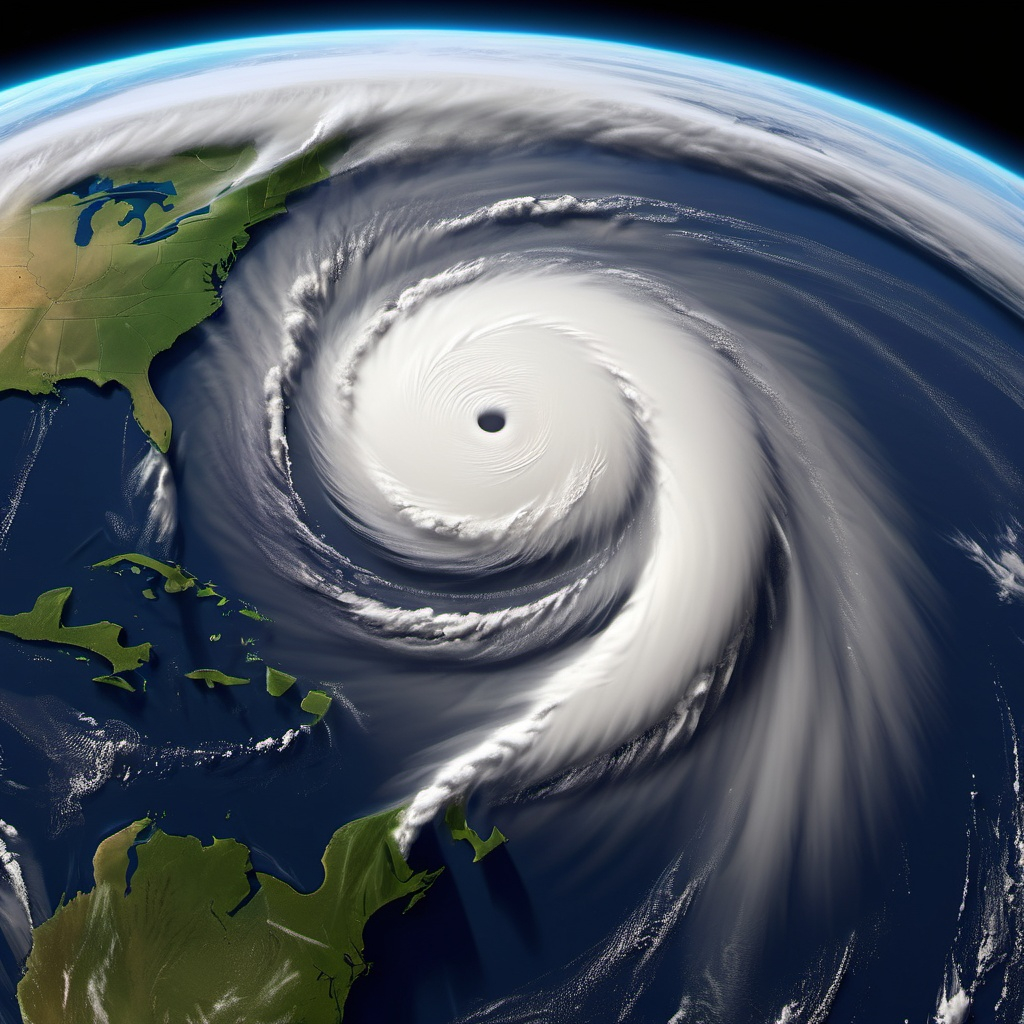
\includegraphics[width=\paperwidth, height=\paperheight]{images/openAIart-hurricane.png}};

%      \begin{scope}[
%        shift={(\pagewidth/2, -15cm)},
%        draw=white,
%        scale=1
%      ]
%        
%        % Define the vector field function
%        % Based on Van der Pol's equation with mu=0.08
%        \def\vectorfieldx(#1,#2){0.08 * (1 - (#2)^2) * (#1) - (#2)}
%        \def\vectorfieldy(#1,#2){(#1)}
%
%        % Draw the vector field
%        \foreach \x in {-10,-9.4,...,10}
%            \foreach \y in {-6,-5.4,...,6}
%            {
%                % Calculate the vector at (\x, \y)
%                \pgfmathsetmacro\vx{\vectorfieldx(\x,\y)}
%                \pgfmathsetmacro\vy{\vectorfieldy(\x,\y)}
%                
%                % Normalize the vector for consistent arrow lengths
%                \pgfmathsetmacro\norm{sqrt(\vx*\vx + \vy*\vy + 0.01)}
%                \pgfmathsetmacro\scaleChange{atan(\norm)/100/\norm}
%                \pgfmathsetmacro\vx{\vx*\scaleChange}
%                \pgfmathsetmacro\vy{\vy*\scaleChange}
%                            
%                % Draw the vector as an arrow
%                \draw[->] (\x,\y) -- ++(\vx,\vy);
%            }
%
%        
%      \end{scope}



		\fill[path fading=north,covershade] (0,2.2in) rectangle ([yshift=-1.01in, xshift=2pt]current page.north east);
		\fill[covershade] (0,-1in) rectangle ([yshift=-1.05in]current page.north east);
%		\fill[path fading=south, covershade] (0,-2in) rectangle ([xshift=1in,yshift=2in]current page.south east);
	\end{scope}




\newcommand{\titletext}[5]{
	\draw (#1, #2) node[right,opacity=0.55] {	
		\textpdfrender{
		    TextRenderingMode=Fill,
		    LineWidth=1pt,
		    FillColor=#4,
		  }{\fontsize{#5}{100}\fontfamily{phv}\selectfont  \bfseries #3}
	};
	\draw (#1, #2) node[right] {	
		\textpdfrender{
		    TextRenderingMode=Stroke,
		    LineWidth=1pt,
		    StrokeColor=#4,
		  }{\fontsize{#5}{100}\fontfamily{phv}\selectfont  \bfseries #3}
	};
}

\newcommand{\subtitletext}[5]{
	\draw (#1, #2) node[right,opacity=0.55] {	
		\textpdfrender{
		    TextRenderingMode=Fill,
		    LineWidth=1pt,
		    FillColor=#4,
		  }{\fontsize{#5}{100}\fontfamily{phv}\selectfont #3}
	};
	\draw (#1, #2) node[right] {	
		\textpdfrender{
		    TextRenderingMode=Stroke,
		    LineWidth=1pt,
		    StrokeColor=#4,
		  }{\fontsize{#5}{100}\fontfamily{phv}\selectfont #3}
	};
}




  \begin{scope}[yscale=-1, xscale=1, x=2.7pt, y=2.7pt,line join=miter,line cap=butt,line width=1.3pt, yshift=2.3cm, xshift=.7cm,
	  ]

	\coordinate (SUB) at (135, 4);

\begin{bookonly}
	\titletext{6}{-5}{Mathematical Modelling}{coverblue}{50}%{58}	
\end{bookonly}

\begin{displayonly}
	\titletext{6}{-5}{Mathematical Modelling}{coverblue}{45}%{50}	
\end{displayonly}


%    \begin{scope}[yscale=-9.7, xscale=9.7, yshift=-.96in]
%	  \fill[coverblue, opacity=.7] \LINEARALGEBRAoutline;
%	  \draw[coverblue, line width=1.3pt] \LINEARALGEBRAoutline;
%    \end{scope}
  \end{scope}
%


  

	\path[white] (SUB) node[anchor=north west] {\Large \bfseries \sffamily \coversubtitle};



\newcommand{\authornames}{\huge \sffamily \bfseries \begin{tabular}{r}Bernardo Galv\~ao-Sousa\end{tabular}}
	\newcommand{\ypadd}{.5em}
	\newcommand{\xpadd}{1em}


\begin{bookonly}
	\draw (0, -24) node[right, xshift=10em] (AUTHOR) {\phantom{\authornames}};	
\end{bookonly}

\begin{displayonly}
	\draw (0, -8.5) node[right, xshift=10em] (AUTHOR) {\phantom{\authornames}};	
\end{displayonly}


	\path let \p1 = (AUTHOR.north) in coordinate (Ab1) at (0,\y1+\ypadd);
	\path let \p1 = (AUTHOR.north east) in coordinate (Ab2) at (\x1+\xpadd,\y1+\ypadd);
	\path let \p1 = (AUTHOR.south east) in coordinate (Ab3) at (\x1+\xpadd,\y1-\ypadd);
	\path let \p1 = (AUTHOR.south) in coordinate (Ab4) at (0,\y1-\ypadd);

	\path[fill=covershade, path fading=west, opacity=.8] (Ab1) -- (Ab2) -- (Ab3) -- (Ab4);
	\draw[covershade!80!black, line width=1.3pt] (Ab1) -- (Ab2) -- (Ab3) -- (Ab4);
\begin{bookonly}
	\draw (0, -24) node[right, xshift=10em, white!75!black] (AUTHOR) {\authornames};
\end{bookonly}
\begin{displayonly}
	\draw (0, -8.5) node[right, xshift=10em, white!75!black] (AUTHOR) {\authornames};
\end{displayonly}

\end{tikzpicture}


\newpage

\begin{bookonly}
	\clearpage
	\hbox{}
	\newpage
	\begin{center}
	{\color{myorange}\huge\bfseries\sffamily Linear Algebra}\\

\vspace{.2in}
{
\it \copyright\,Jason Siefken, 2016--2022 \\
Creative Commons By-Attribution Share-Alike\, \makebox(30,5){
\includegraphics[height=1.2em]{by-sa.pdf}}
}
\end{center}

\section*{About this Book}

\subsection*{For the student}

This book is your introductory guide to linear algebra. It is divided into
\emph{modules}, and each module is further divided into \emph{exposition},
\emph{practice problems}, and \emph{core exercises}.

The \emph{exposition} is easy to find---it's the text that starts each
module and explains the big ideas of linear algebra.  The \emph{practice
problems} immediately follow the exposition and are there so you can
practice with concepts you've learned.  Following the practice problems
are the \emph{core exercises}. The core exercises build up, through
examples, the concepts discussed in the exposition.

To optimally learn from this text, you should:
\begin{itemize}
	\item Start each module by reading through the \emph{exposition} to get familiar with the main ideas and 
		linear algebra terminology.

	\item Work through the \emph{core exercises} to develop an understanding and intuition behind the main ideas
		and their subtleties.

	\item Re-read the \emph{exposition} and identify which concepts each core exercise connects with.

	\item Work through the \emph{practice problems}. These will serve as a check on whether you've understood
		the main ideas well enough to apply them.
\end{itemize}

{\bf The core exercises.} Most (but not all) core exercises will be
worked through during lecture time, and there is space for you to work
provided after each
of the core exercises. The point of the core exercises is to develop the main ideas of
linear algebra by exploring examples. When working on core exercises, think
``it's the journey that matters not the destination''. The
answers are not the point! If you're struggling, keep with it. The
concepts you struggle with you remember well, and if you look up the
answer, you're likely to forget just a few minutes later. 

{\bf So many definitions.} A big part of linear algebra is learning precise and
technical language\footnote{ Beyond three dimensions, things get very confusing
very quickly.  Having precise definitions allows us to make arguments that
rely on logic instead of intuition; and logic works in all dimensions.}.
There are many terms and definitions you need to learn, and by far the
best way to successfully learn these terms is to understand where they
come from, why they're needed, and practice using them. That is, don't
try to memorize definitions word for word. Instead memorize the idea
and \emph{reconstruct} the definition; go through the core exercises and
identify which definitions appear where; and explain linear algebra to
others using these technical terms.

{\bf Contributing to the book.} Did you find an error? Do you
have a better way to explain a linear algebra concept? Please,
contribute to this book!  This book is open-source, and we welcome
contributions and improvements. To contribute to/fix part of
this book, make a \emph{Pull Request} or open an \emph{Issue} at
\url{https://github.com/siefkenj/IBLLinearAlgebra}. If you contribute,
you'll get your name added to the contributor list.


\subsection*{For the instructor}

This book is designed for a one-semester introductory linear algebra course
course with a focus on geometry (MAT223 at the University of Toronto). 
It has not been designed for an ``intro to proofs''-style course, but could be adapted for one.

Unlike a traditional textbook that is grouped into chapters and sections
by subject, this book is grouped into modules. Each module contains exposition
about a subject, practice problems (for students to work on by themselves), and core exercises
(for students to work on with your guidance). Modules group related concepts, but the 
modules have been designed to facilitate learning linear algebra rather than to serve
as a reference. For example, information about change-of-basis is spread across several non-consecutive
modules; each time change-of-basis is readdressed, more detail is added.

{\bf Using the book.} This book has been designed for use in large 
active-learning classrooms driven by a \emph{think, pair-share}/small-group-discussion format.
Specifically, the \emph{core exercises} (these are the problems which aren't labeled ``Practice Problems''
and for which space is provided to write answers) are designed for use during class time.

A typical class day looks like:
\begin{enumerate}
	\item {\bf Student pre-reading.} Before class, students will read through the relevant module.

	\item {\bf Introduction by instructor.} This may involve giving a definition,
		a broader context for the day's topics, or answering questions.

	\item {\bf Students work on problems.} Students work individually or in pairs/small groups
		on the prescribed core exercise. During this time the instructor moves
		around the room addressing questions that students may have and giving
		one-on-one coaching.

	\item {\bf Instructor intervention.} When most students have successfully solved
		the problem, the instructor refocuses the class by providing an
		explanation or soliciting explanations from students.
		This is also time for the instructor to ensure that everyone has
		understood the main point of the exercise (since it is sometimes
		easy to miss the point!).

		If students are having trouble, the instructor can give hints
		and additional guidance to ensure students' struggle is productive.

	\item {\bf Repeat step 3.}
\end{enumerate}

Using this format, students are thinking (and happily so) most of the class. Further,
after struggling with a question, students are especially primed to hear the insights of the instructor.

{\bf Conceptual lean.}
The \emph{core exercises} are geared towards concepts instead of computation, though some core exercises
focus on simple computation. They also have a geometric lean. Vectors are initially
introduced with familiar coordinate notation, but eventually, coordinates are understood to be
\emph{representations} of vectors rather than ``true'' geometric vectors, and objects like the
determinant are defined via oriented volumes rather than formulas involving matrix entries.

Specifically lacking are exercises focusing on the mechanical skills of row reduction and
computing matrix inverses. Students must practice these skills, but they require little instructor
intervention and so can be learned outside of lecture (which is why core exercises don't focus on
these skills).

{\bf How to prepare.}
Running an active-learning classroom is less scripted than lecturing.
The largest
challenges are: (i) understanding where students are at, (ii) figuring out what to do given the current
understanding of the students, and (iii) timing.

To prepare for a class day, you should:
\begin{enumerate}
	\item {\bf Strategize about learning objectives.} Figure out what the point of the day's lesson is
		and brain storm some examples that would illustrate that point.
	\item {\bf Work through the core exercises.} 
	%	By working through the exercises yourself, you
	%	will be ready to build off student reasoning, and better able to direct a class towards
	%	the important ideas\footnote{ The content of linear algebra is fairly non-linear. One of the hardest parts
	%	of teaching linear algebra is coming up with an explanation that only depends on ideas that have already been taught.}.
	\item {\bf Reflect.} Reflect on how each core exercise addresses the day's goals. Compare with the examples you
		brainstormed and prepare follow-up questions that you can use in class to test for understanding.
	\item {\bf Schedule.} Write timestamps next to each core exercise indicating at what minute you hope
		to start each exercise. Give more time for the exercises that you judge as foundational, and be prepared
		to triage. It's appropriate to leave exercises or parts of exercises for homework, but change the order
		of exercises at your peril---they really do build on each other.
\end{enumerate}

A typical
50 minute class is enough to get through 2--3 core exercises (depending on the difficulty), and class observations
show that class time is split 50/50 between students working and instructor explanations.

\subsection*{License}
 Unless otherwise mentioned, pages of this document are licensed under
the Creative Commons By-Attribution Share-Alike License. That means, you are free
to use, copy, and modify this document provided that you provide attribution to the
previous copyright holders and you release your derivative work under the same license.
Full text of the license is at \url{http://creativecommons.org/licenses/by-sa/4.0/}

If you modify this document, you may add your name to the copyright list. Also,
if you think your contributions would be helpful to others, consider making a
pull request, or opening an \emph{issue} at \url{https://github.com/siefkenj/IBLLinearAlgebra}

{\bf Incorporated content.}
Content from other sources is reproduced here with permission and retains the
Author's copyright. Please see the footnote of each page to verify the
copyright.

Included in this text are tasks created by the Inquiry-Oriented Linear Algebra (IOLA) project. Details
about these tasks can be found on their website \url{http://iola.math.vt.edu/}. Also included are some
practice problems from Beezer's \emph{A First Course in Linear Algebra} (marked with the symbol \beezer next to the
problem), and from Hefferon's \emph{Linear Algebra} (marked with the symbol \hefferon next to the problem).

{\bf Contributing.} You can report errors in the book or contribute to the book by filing an \emph{Issue} or
a \emph{Pull Request} on the book's GitHub page: \url{https://github.com/siefkenj/IBLLinearAlgebra/}


	\section*{Contributors}
	% sorting code from
% http://tex.stackexchange.com/questions/121489/alphabetically-display-the-items-in-itemize
\newcommand{\sortitem}[2][\relax]{%
  \DTLnewrow{list}% Create a new entry
  \ifx#1\relax
    \DTLnewdbentry{list}{sortlabel}{#2}% Add entry sortlabel (no optional argument)
  \else
    \DTLnewdbentry{list}{sortlabel}{#1}% Add entry sortlabel (optional argument)
  \fi%
  \DTLnewdbentry{list}{description}{#2}% Add entry description
}
\newenvironment{sortedlist}{%
  \DTLifdbexists{list}{\DTLcleardb{list}}{\DTLnewdb{list}}% Create new/discard old list
}{%
  \DTLsort{sortlabel}{list}% Sort list
  \begin{itemize*}[label={\color{mypink}$\circ$}]%
    \DTLforeach*{list}{\theDesc=description}{%
      \item \theDesc}% Print each item
  \end{itemize*}%
}

This book is a collaborative effort.  The following people have contributed
to its creation:
\begin{quote}
\begin{sortedlist}
	\sortitem[Wang]{Tianhao (Patrick) Wang}
	\sortitem[Khan]{Sameul Khan}
	\sortitem[King]{Avery King}
	\sortitem[Frohlich]{Jesse Frohlich}
	\sortitem[Wolske]{Zack Wolske}
	\sortitem[Le]{Dan Le}
	\sortitem[Qiu]{Ruo Ning (Nancy) Qiu}
    \sortitem[Li]{Xintong (Alucart) Li}
    \sortitem[Chen]{Shukui Chen}
    \sortitem[Kim]{Julia Kim}
    \sortitem[El-Sheikha]{Hassan El-Sheikha}
    \sortitem[Wang]{Robert Wang}
\end{sortedlist}
{\color{mypink}$\circ$}
\end{quote}

%	\section*{Dedication}
%	\begin{center}
%		This book is dedicated to
%		\href{https://www.gazettetimes.com/news/local/obituaries/dr-robert-main-burton/article_9c087f07-c005-515a-bb3f-2c9c6a6b7332.html}{\color{blue}Dr.~Bob Burton}---friend and mentor.
%
%		\emph{\large ``Sometimes you have to walk the mystical path with practical feet.''}
%	\end{center}
	\newpage
	\mbox{}
	{
		\pagestyle{empty}
		\setcounter{tocdepth}{1}
		\tableofcontents
		\thispagestyle{empty}
	}
	\newpage
	\mbox{}
	\newpage
\end{bookonly}

\setcounter{page}{1}
\pagestyle{siefken}


\addcontentsline{toc}{chapter}{Lessons}


\phantomsection
\addcontentsline{toc}{section}{Introduction}


\begin{module}\label{module1}
	\Title{Modeling}

	In this module you will learn
	\begin{itemize}
		\item ??
	\end{itemize}

	\Heading{Modeling}

Suppose you are observing some \emph{green} ants walking on the sidewalk.
In the first minute you record 10 ants. In the second minute you
record 20. In the third minute, you record 40 ants. This continues until
there are too many ants for you to count.

\begin{center}
	\begin{tabular}{c|c}
		Minute & \#Green Ants\\
		\hline
		1 & 10\\
		2 & 20\\
		3 & 40\\
		4 & 80\\
		$\vdots$ & $\vdots$
	\end{tabular}
\end{center}

Since you lost count of the ants, you decide to use mathematics to try and figure out
how many ants walked by on minutes $5$, $6$, \ldots. You notice the pattern that
\[
	\text{Green ants per minute $n$} = 2^{n-1}\cdot 10.
\]
Stupendous! Mathematics now predicts there were $160$ ants during minute $5$. But something
else catches your eye. Across the sidewalk are \emph{brown} ants. You count these
ants every minute.

\begin{center}
	\begin{tabular}{c|c}
		Minute & \#Brown Ants\\
		\hline
		1 & 3\\
		2 & 6\\
		3 & 12\\
		4 & 24\\
		$\vdots$ & $\vdots$
	\end{tabular}
\end{center}

The pattern is slightly different. This time, 
\[
	\text{Green ants per minute $n$} = 2^{n-1}\cdot 3.
\]

Your friend, who was watching you the whole time, looks confused. ``Why come up with two complicated equations
when you can describe both types of ant at once?'' they declare.

\begin{center}
	\begin{tabular}{c}
		$\text{\#Ants at minute $n$}\ =\ 2\cdot(\text{\#Ants at minute $n-1$})$\\
		$\text{\#Green ants at minute 1}=10$\\
		$\text{\#Brown ants at minute 1}=3$\\
	\end{tabular}
\end{center}

Your friend has a point. Their model is elegant, but \emph{your} model can predict how many ants pass by at minute $3.222$!
Though, your friend would probably complain that $46.654$ is not a number of ants\ldots.

\medskip

You and your friend have just come up with two different \emph{mathematical models} for the number of ants
that walk across the sidewalk. They happen to make similar predictions for each minute and each have their
strengths and weakenesses. In this course, we will be focused on a particular type of mathematical model---one
that uses \emph{differential equations} at its core.

\Heading{Types of Models}

\begin{definition}[Mathematical Model]
A \emph{mathematical model}\index{model} is a description of the world
	\begin{enumerate}
		\item created in the service of answering a question, and
		\item where the complexity of the world has been abstracted away to numbers, quantities, and their relationships\footnote{ Other
mathematical objects are also allowed.}.
	\end{enumerate}
\end{definition}

In the previous situation, the \emph{question} you were trying to answer was ``how many ants are there at a given minute?''.
We sidestepped difficult issues like, ``Is an ant that is missing three legs still an ant?'' by using the common-sense
convention that ``the number of ants is a whole number and one colored blob that moves under its own power corresponds to one ant''; thus,
we could use single numbers to represent our quantity of interest (the ants).

You and your friend already came up with two types of models.
\begin{itemize}
	\item An \textbf{analytic} model based on known functions.
	\item A \textbf{recursive} model where subsequent terms are based on previous terms and initial conditions.
\end{itemize}

If we define $A(n)$ to be the number of ants corssing the sidewalk at minute $n$, the \emph{analytic} model presented for green ants is
\[
	A(n)=2^{n-1}\cdot 10
\]
and the \emph{recursive} model presented is
\begin{align*}
	A(1) &= 10\\
	A(n) &= 2\cdot A(n-1).
\end{align*}

Each type of model has pros and cons. For example, the analytic model allows you to calculate the number of ants at any minute
with few button presses on a calculator, whereas the recursive model is more difficult to calculate but
makes it clear that the number of ants is doubling every minute.

Often times recursive models are easier to write down than analytic models\footnote{ In fact, in many real-world situations, an analytic model
doesn't exist}, but they maybe harder to analyze. A third type of model has similarities to both analytic and recursive models, and
brings the power of calculus to modeling.

\begin{itemize}
	\item A \textbf{differential-equations} model is a model based on a relationship between a function's derivative(s), its values, and initial conditions.
\end{itemize}

\emph{Differential-equations} models are useful because derivatives correspond to rates of change---and things in the world are always changing.
Let's try to come up with a differential equations model for the ants.

We'd like an equation relating $A(n)$, the number of ants at minute $n$, to $A'(n)$, the \emph{instantaneous rate of change} of the number of ants at minute $n$.
Making a table, we see

\begin{center}
	\begin{tabular}{c|c|c}
		Minute & \#Brown Ants & Change (from prev. minute)\\
		\hline
		1 & 3 & ?\\
		2 & 6 & 3\\
		3 & 12 & 6\\
		4 & 24 & 12\\
	\end{tabular}
\end{center}

or

\begin{center}
	\begin{tabular}{c|c|c}
		Minute & \#Brown Ants & Change (from next minute)\\
		\hline
		1 & 3 & 3\\
		2 & 6 & 6\\
		3 & 12 & 12\\
		4 & 24 & ?\\
	\end{tabular}
\end{center}

depending on whether we record the change from the previous minute or up to the subsequent minute. Neither table gives the \emph{instantaneous} rate of
change, but in both tables, the change is proportional to the number of ants. So, we can set up a model
\[
	A'(n) = kA(n)
\]
where $k$ is a constant of proportionality that we will try to determine later. We've just written down a \emph{differential equation} with an undetermined parameter, $k$.

\begin{definition}[Differential Equation]
	A \emph{differential equation}\index{differential equation} is an equation relating a function to one or more of its derivatives.
\end{definition}

We'd like to figure out what $k$ is. One way to do so is to solve the differential equation and find the values of $k$ so that our model
correctly predicts the data. This is called \emph{fitting} the model to data.

\begin{definition}[Fitting a Model]
	Given a model $M$ with parameters $k_1$, $k_2$, $\ldots$ and data $D$, \emph{fitting the model $M$ to the data $D$}
	is the process of finding values for the parameters $k_1$, $k_2$, $\ldots$ so that $M$ most accurately predicts the data $D$.
\end{definition}

Note that, in general, fitting a model to data doesn't necessarily produce \emph{unique} values for the unknown parameters, and a fitted model
(especially when the data comes from real-world observations) usually doesn't reproduce the data exactly. However, in the case of these ants, we
just might get lucky.

\Heading{Solving Differential Equations}

In general, \emph{there is no algorithm for solving differential equations}. Fortunately, it is easy to check whether any particular
function is a solution to a differential equation, since there \emph{is} an algorithm to differentiate functions\footnote{ More specifically, there is an algorithm
to differentiate the \emph{elementary} functions, those functions formed by compositions, sums, products, and quotients of polynomials, trig, exponentials, and logs.}.
Because of this, \emph{guess and check} will be our primary method for solving differential equations.

\begin{example}
Use educated guessing to solve $A'(n)=kA(n)$.

Since $A'\approx A$, we might start with a function that is equal to its own derivative. There is a famous one: $e^n$. Testing, we see
\[
	\frac{\d}{\d n}e^n=e^n=ke^n
\]
if $k=1$, but it doesn't work for other $k$'s. Trying $e^{kn}$ instead yields
\[
	\frac{\d}{\d n}e^{kn}=ke^{kn}
\]
which holds for all $k$. Thus $A(n)=e^{kn}$ is \emph{a} solution to $A'(n)=kA(n)$. However, there are other solutions, because
\[
	\frac{\d}{\d n}Ce^{kn}=C\left(ke^{kn}\right)=k\left(Ce^{kn}\right),
\]
and so for every $C$, the function $A(n)=Ce^{kn}$ is a solution to $A'(n)=kA(n)$.
\end{example}

By guessing-and-checking, we have found an infinite number of solutions to $A'(n)=kA(n)$.  It's now time to fit our
model to the data.

\begin{example}
	Find values of $C$ and $k$ so that $A(n)=Ce^{kn}$ best models brown ants.

	Taking two rows from our brown ants table, we see
	\begin{align*}
		A(1) &= Ce^{k} = 3\\
		A(2) & = Ce^{2k}=6.
	\end{align*}

	Since $e^k$ can never be zero, from the first equation we get $C=3/e^k$. Combining with the second equation we find
	\[
		Ce^{2k}=\frac{3}{e^k}e^{2k}=3e^k=6
	\]
	and so $e^k=2$. In other words $k=\ln 2$. Plugging this back in, we find $C=3/2$. Thus our fitted model is
	\[
		A(n)=\tfrac{3}{2}e^{n\ln 2}.
	\]
\end{example}

Upon inspection, we can see that $\tfrac{3}{2}e^{n\ln 2} = 3\cdot 2^{n-1}$, which is the analytic model
that was first guessed for brown ants.



%One of the beauties of the guess-and-check method is that it \emph{cannot} produce an incorrect answer,
%since you're always checking (though it may fail to produce answers, any answer that it \emph{does} produce
%will be correct). Thus, even if you did some mathematically-dubious steps to produce a guess, if it passes the checks,
%the final answer is valid.
%
%\begin{example}
%Use Leibniz notation, integral calculus, and guess-and-check to come up with solutions to $A'(n)=kA(n)$.
%
%In Leibniz notation, $A'(n)$ is written as $\displaystyle\frac{\d A}{\d n}$, and we may suppress the function variable and write $A$ in place of $A(n)$. Thus, our equation becomes
%\[
%	\frac{\d A}{\d n}=kA.
%\]
%Treating $\d A/\d n$ as an actual ratio, we can bring all $A$'s to the left and $n$'s to the right, giving
%\[
%	\frac{1}{A}\d A = k\d n.
%\]
%Integrating both sides gives
%\[
%	\int \frac{1}{A}\d A = \ln A + C_1 \qquad =\qquad  \int k\d n = kn + C_2,
%\]
%and so
%\[
%	\ln A + C_1 = kn + C_2 \qquad \iff \qquad \ln A = kn + (C_2-C_1) = kn + C_3.
%\]
%Solving for $A$ by exponentiating both sides gives
%\[
%	A = e^{\ln A} = e^{kn + C_3} = C_4 e^{kn}.
%\]
%Much of what we've done in the preceding calculation \emph{was not rigorous mathematics}, but that's okay, because
%it leads us to the guess: $A(n)=Ce^{kn}$. Finally, we can test our guess and verify
%\[
%	\frac{\d}{\d n}Ce^{kn}=C\left(ke^{kn}\right)=k\left(Ce^{kn}\right),
%\]
%and so $A(n)=Ce^{kn}$ is a solution for every $C$.\footnote{ Notice that in our ``guess work'', $C_4$ was actually restricted to be a positive
%number, but our solution works with $C$ being positive or negative.}
%
%\end{example}




	%\begin{exercises}
		% Topics:
		% Sets, set builder notation, set operations,
		% vectors \& scalars, vector notation, vectors \& points, vector arithmetic,
		% coordinates \& the standard basis, higher dimensions,
	\begin{problist}
		% Computation (4 questions)
		\prob
		\begin{enumerate}
			\item
			Write the following vectors as column vectors.
			\begin{enumerate}
				\item $4\xhat -3\zhat +2\yhat -2\xhat\in\R^3$.
				\item $\yhat +\xhat -5\yhat \in\R^2$.
			\end{enumerate}
			\item
			Write the following vectors as linear combinations of
			$\xhat$, $\yhat$, and $\zhat$.
			\begin{enumerate}
				\item $\mat{1\\-2\\3}$.
				\item $\mat{-2\\5\\4} + \mat{1\\-2\\ -5} + \mat{1\\0\\1}$.
			\end{enumerate}
		\end{enumerate}
		% Q1 Solution
		\begin{solution}
			\begin{enumerate}
				\item
				\begin{enumerate}
					\item $\mat{2\\2\\-3}$
					\item $\mat{1\\-4}$
				\end{enumerate}
				\item
				\begin{enumerate}
					\item $\xhat - 2\yhat + 3\zhat$
					\item $3\yhat$
				\end{enumerate}
			\end{enumerate}
		\end{solution}

		\prob
		Compute
		\[
			3\mat{2\\-1\\1\\1\\0}+
			(-2)\mat{1\\2\\-7\\3\\0}+
			\mat{-3\\3\\9\\2\\2}
		\]
		% Q2 Solutions
		\begin{solution}
		    $\mat{1\\-4\\26\\-1\\2}$
		\end{solution}

		\prob[\hefferon[2.21,2.22]]
		Decide if the vector is in the set. If it is, what value of the
		parameters produce that vector?
		\begin{enumerate}
			\item $\mat{5\\-5}$ and the set
			\[
				\Set*{\vec{v}\in\R^2 \given \vec{v}=k\mat{1\\-1} \text{ for some } k\in\R}
			\]
			\item $\mat{-1\\2\\1}$ and the set
			\[
				\Set*{\vec{v}\in\R^3 \given
				\vec{v}=i\mat{-2\\1\\0}+j\mat{3\\0\\1} \text{ for some } i,j\in\R}
			\]
			\item $\mat{3\\-1}$ and the set
			\[
				\Set*{\vec{v}\in\R^2 \given \vec{v}=k\mat{-6\\2} \text{ for some } k\in\R}
			\]
			\item $\mat{5\\4}$ and the set
			\[
				\Set*{\vec{v}\in\R^2 \given \vec{v}=j\mat{5\\-4} \text{ for some } j\in\R}
			\]
			\item $\mat{2\\1\\-1}$ and the set
			\[
				\Set*{\vec{v}\in\R^3 \given \vec{v}=r\mat{1\\-1\\3}+\mat{0\\3\\-7} \text{ for some } r\in\R}
			\]
			\item $\mat{1\\0\\1}$ and the set
			\[
				\Set*{\vec{v}\in\R^3 \given \vec{v}=j\mat{2\\0\\1}+k\mat{-3\\-1\\1} \text{ for some } j,k\in\R}
			\]
		\end{enumerate}
		% Q3 solution
		\begin{solution}
			\begin{enumerate}
		        \item Yes, take $k=5$.
		        \item Yes, take $i=2,j=1$.
		        \item Yes, take $k=-\frac{1}{2}$.
		        \item No.
		        \item Yes, take $r=2$.
		        \item No.
		    \end{enumerate}
		\end{solution}

		% Conceptual (3 questions)
		\prob
		% Purpose: get students to understand (the beginnings of) scale-invariance
		% of bases, as well as carefully reading mathematical expressions.
		Draw the following subsets of $\R^2$ and then determine which are equal or subsets of each other.
		\begin{enumerate}
			\item $A=\Set*{\vec v\in\R^2\given \vec v=n\mat{2\\1}\text{ for some integer }n\in\Z}$
			\item $B=\Set*{\vec v\in\R^2\given \vec v=t\mat{4\\2}\text{ for some }t\in\R}$
			\item $C=\Set*{\vec v\in\R^2\given \vec v=n\mat{4\\2}\text{ for some integer }n\in\Z}$
			\item $D=\Set*{\vec v\in\R^2\given \vec v=t\mat{2\\1}\text{ for some }t\in\R}$
		\end{enumerate}
		\begin{solution}
			\begin{enumerate}
				\item 
				\begin{tikzpicture}[baseline = (current bounding box.north)]
					\begin{axis}[
						anchor=origin,
						disabledatascaling,
						xmin=-4,xmax=4,
						ymin=-4,ymax=4,
						xtick={-4,-2,0,2,4},
						ytick={-4,-2,0,2,4},
						x=0.5cm,y=0.5cm,
						grid=both,
						grid style={line width=.1pt, draw=gray!10},
						axis lines=middle,
						minor tick num=0,
						enlargelimits={abs=1.0},
						axis line style={latex-latex},
						ticklabel style={font=\tiny,fill=white},
						xlabel style={at={(ticklabel* cs:1)},anchor=north west},
						ylabel style={at={(ticklabel* cs:1)},anchor=south west}
					]
					\end{axis}
					\foreach \n in {-2,...,2} {
						\fill [mypink] (\n,\n/2) circle[radius=2pt];
					}
				\end{tikzpicture}
				\item 
				\begin{tikzpicture}[baseline = (current bounding box.north)]
					\begin{axis}[
						anchor=origin,
						disabledatascaling,
						xmin=-4,xmax=4,
						ymin=-4,ymax=4,
						xtick={-4,-2,0,2,4},
						ytick={-4,-2,0,2,4},
						x=0.5cm,y=0.5cm,
						grid=both,
						grid style={line width=.1pt, draw=gray!10},
						axis lines=middle,
						minor tick num=0,
						enlargelimits={abs=1.0},
						axis line style={latex-latex},
						ticklabel style={font=\tiny,fill=white},
						xlabel style={at={(ticklabel* cs:1)},anchor=north west},
						ylabel style={at={(ticklabel* cs:1)},anchor=south west}
					]
						\draw [mygreen, thick] (-5,-2.5) -- (5,2.5);
					\end{axis}
				\end{tikzpicture}
				\item 
				\begin{tikzpicture}[baseline = (current bounding box.north)]
					\begin{axis}[
						anchor=origin,
						disabledatascaling,
						xmin=-4,xmax=4,
						ymin=-4,ymax=4,
						xtick={-4,-2,0,2,4},
						ytick={-4,-2,0,2,4},
						x=0.5cm,y=0.5cm,
						grid=both,
						grid style={line width=.1pt, draw=gray!10},
						axis lines=middle,
						minor tick num=0,
						enlargelimits={abs=1.0},
						axis line style={latex-latex},
						ticklabel style={font=\tiny,fill=white},
						xlabel style={at={(ticklabel* cs:1)},anchor=north west},
						ylabel style={at={(ticklabel* cs:1)},anchor=south west}
					]
					\end{axis}
					\foreach \n in {-1,...,1} {
						\fill [mypink] (\n*2,\n) circle[radius=2pt];
					}
				\end{tikzpicture}
				\item 
				The set $D$ and $B$ are equal.
			\end{enumerate}
			We have $C\subseteq A$, $C\subseteq B$, $C\subseteq D$,  $A\subseteq B$, $A\subseteq D$, and $B=D$.
		\end{solution}

		\prob
		Let $\vec a=\mat{1\\2}$, $\vec b=\mat{2\\4}$, $\vec c=\xhat+3\yhat$, and $\vec d=\vec a+\vec c$.
		\begin{enumerate}
			\item Is $\xhat$ a linear combination of $\vec a$ and $\vec b$?
			\item Is $\vec d$ a linear combination of $\vec a$ and $\vec b$?
			\item Is $\vec p=\mat{1\\1}$ a linear combination of $\vec a$ and $\vec c$?
			\item Is $\vec q=\mat{-3\\3}$ a linear combination of $\vec a$, $\vec b$, $\vec c$, and $\vec d$?
		\end{enumerate}
		% Q5 Solutions
		\begin{solution}
            \begin{enumerate}
    		    \item No.
    		    \item No.
    		    \item Yes.
    		    \item Yes.
		    \end{enumerate}
		\end{solution}
		
		\prob
		Use set-builder notation to describe the following sets.
		\begin{enumerate}
			\item The set of vectors in $\R^{2}$ whose coordinates are rational numbers.

			\item The set of vectors in $\R^{2}$ whose coordinates are irrational
				numbers.

			\item Let $P(\vec x) = -\vec x$. The set $\Set*{P(\vec e_{1}), P(\vec e_{2})}$.
		\end{enumerate}
		\begin{solution}
			\begin{enumerate}
				\item $\Set*{\vec{v}\in\R^2 \given \vec{v}=\mat{\alpha\\\beta} \text{ for some } \alpha,\beta\in\Q}$
				\item $\Set*{\vec{v}\in\R^2 \given \vec{v}=\mat{\alpha\\\beta} \text{ for some } \alpha,\beta\in\R\setminus\Q}$
				\item $\Set*{\vec{v}\in\R^2 \given \vec{v}=-\vec{e}_1 \text{ or } \vec{v}=-\vec{e}_2}$
			\end{enumerate}
		\end{solution}

		% Challenge (3 questions)
		\prob % Propose: get students to understand quantifiers and set operations
		% practice providing justification to their intuitive guesses
		Which of the following statements are true about the set listed below? Justify your
		answers.
		\begin{enumerate}
			\item $\mathcal{Y}$, the $y$-axis in $\R^{3}$.
				\begin{enumerate}
					\item $\mathcal{Y}$ is a finite set.

					\item Let
						\[
							\mathcal{A} = \Set*{\vec a \in \R^3 \given \vec a = \beta \vec v
										  \text{ for some } \vec v \in \mathcal{Y}, \beta \in \R},
						\]
						then $\mathcal{A} \subseteq \mathcal{Y}$.

					\item For all vectors $\vec v \in \mathcal{Y}$, we have $\vec v \neq
						\vec 0$.

					\item For some vectors $\vec v \in \mathcal{Y}$, we have $\vec v
						\neq \vec 0$.

					\item For all vectors $\vec v \in \mathcal{Y}$, there exists a vector
						$\vec x \in \mathcal{Y}$ such that $\vec x + \vec v = \vec e_{2}$.

					\item There exists a vector $\vec x \in \mathcal{Y}$ such that for
						all vectors $\vec v \in \mathcal{Y}$, we have $\vec x + \vec v =
						\vec e_{2}$.
				\end{enumerate}

			\item $\mathcal{S}$, the set of vectors in $\R^{3}$ whose coordinates are $\pm3$.
				\begin{enumerate}
					\item $\mathcal{S}$ is a finite set.

					\item Let
					\[
						\mathcal{A} = \Set*{\vec a \in \R^3 \given \vec a = \beta \vec v
									  \text{ for some } \vec v \in \mathcal{S}, \beta \in \R },
					\]
					then $\mathcal{A} \subseteq \mathcal{S}$.

					\item For all vectors $\vec v \in \mathcal{S}$, we have $\vec v \neq
						\vec 0$.

					\item For some vectors $\vec v \in \mathcal{S}$, we have $\vec v
						\neq \vec 0$.

					\item For all vectors $\vec v \in \mathcal{S}$, there exists a vector
						$\vec x \in \mathcal{S}$ such that $\vec x + \vec v = \vec 0$.

					\item There exists a vector $\vec x \in \mathcal{S}$ such that for
						all vectors $\vec v \in \mathcal{S}$, we have $\vec x + \vec v =
						\vec 0$.
				\end{enumerate}
		\end{enumerate}
		\begin{solution}
			\begin{enumerate}
				\item 
				\begin{enumerate}
					\item False.
					\item True.
					\item False.
					\item True.
					\item True.
					\item False.
				\end{enumerate}
				\item 
				\begin{enumerate}
					\item True.
					\item False.
					\item True.
					\item True.
					\item True.
					\item False.
				\end{enumerate}
			\end{enumerate}
		\end{solution}

		\prob % Propose: Give students some practices on proving general statements about sets
		For each of the following statements, determine whether it is correct or not. If
		it is, prove it. Otherwise, give a counterexample.
		\begin{enumerate}
			\item If $A \subseteq B$, then $A \cap B = A$.

			\item If $B \subseteq A$, then $A \cap B = A$.

			\item If $A \subseteq B$, then $A \cap B \neq B$.

			\item If $B \subseteq A$, then $A \cap B \neq B$.

			\item If $C \subseteq A \cap B$, then $C \subseteq A$.

			\item If $C \subseteq A \cup B$, then $C \subseteq A$.

			\item If $C \subseteq A \cup B$ and $C \subseteq B$, then $A \cap B
				\subseteq C$.
		\end{enumerate}
		\begin{solution}
			\begin{enumerate}
				\item Correct.
				\item Incorrect.
				\item Incorrect.
				\item Incorrect.
				\item Correct.
				\item Incorrect.
				\item Incorrect.
			\end{enumerate}
		\end{solution}
	\end{problist}
\end{exercises}

\end{module}





\begin{slide}

\question 

\begin{parts}
	\item What is modelling?
\end{parts}



\begin{solution}
	\begin{itemize}
		\item A precise description of a system
		\item A formal summary of knowledge
		\item A tool that enables prediction
		\item An abstraction suitable for a particular purpose or question
		\item Modelling is a scientific method with ``hypothesis'' in a mathematical form	
	\end{itemize}	
\end{solution}
	
\end{slide}




\begin{slide}
\begin{parts}
\setcounter{partsitem}{1}
	\item Modelling Procedure -- DABAR \footnote{based on the \href{SIAM $M^2 (GS)^2$ Textbook}{https://m3challenge.siam.org/wp-content/uploads/siam-guidebook-final-press.pdf}.}
	
	\begin{enumerate}
		\item[\it Step 1.] \textbf{\large D}efine the problem 
			\begin{solution}\hfill (ask a question)\end{solution}

		\item[\it Step 2.] make \textbf{\large A}ssumptions 
			\begin{solution}\hfill (select a modelling approach)\end{solution}

		\item[\it Step 3.] \textbf{\large B}uild a model
			\begin{solution} \hfill (formulate the model)\end{solution}

		\item[\it Step 4.] \textbf{\large A}ssess the model 
			\begin{solution} \hfill (solve the model) \end{solution}

		\item[\it Step 5.] \textbf{\large R}eport results
			\begin{solution} \hfill (answer the question) \end{solution}
	\end{enumerate}	
\end{parts}

	
\end{slide}




\begin{slide}

\begin{parts}
\setcounter{partsitem}{2}

	\item Course topics:

\begin{itemize}
	\item \hyperref[sec:optimization]{Optimization models}
	\item \hyperref[sec:dynamical]{Dynamical models}
	\item \hyperref[sec:probability]{Probability models}
\end{itemize}
	
\end{parts}

\end{slide}






%\
%%%%%%%%%%%%%%%%%%%%%%%%%%%%%%%%%%%%%%%%%%%%%%%%%%%%%
%
%
%  	OPTIMIZATION MODELS
%
%
%%%%%%%%%%%%%%%%%%%%%%%%%%%%%%%%%%%%%%%%%%%%%%%%%%%%%

\phantomsection
\addcontentsline{toc}{section}{Optimization Models}\label{sec:optimization}




%%%%%%%%%%%%%%%%%%%%%%%%%%%%%%%%%%%%%%%%%%%%%%%%%%%%%
%
%
%  	OPTIMIZATION MODELS
%
%
%%%%%%%%%%%%%%%%%%%%%%%%%%%%%%%%%%%%%%%%%%%%%%%%%%%%%




\begin{slide}

\begin{slidesonly}
	\vspace{3cm}
\end{slidesonly}

\begin{center}
\Huge 
\textcolor{LimeGreen}{Optimization Models}
\end{center}

	
\end{slide}




\addcontentsline{toc}{subsection}{Unconstrained Optimization}

\begin{slide}

\question

\begin{problem}[Optimization Problem\footnote{Adapted from ``Mathematical Modelling'' by Meerschaert.}]
A pig weighting 90 kg gains 3 kg per day and cost 45 cents a day to keep. The market price for pigs is 65 cents/kg, but is falling at 1 cent per day. When should the pig be sold?	
\end{problem}

Introduce variables:
\begin{itemize}
	\item $t=$ time at which the pig is sold (in days)
	\item $w=$ weight of the pig (in kg)
	\item $m=$ market price of a pig (in \$/kg)
	\item $C=$ cost of keeping the pig (in \$)
	\item $R=$ revenue from selling the pig (in \$)
	\item $P=$ profit from the sale of the pig (in \$)
\end{itemize}
	

\begin{parts}
	\item Which of these variables depend on $t$? Based on the statement, what do we know about their values?
	\item What is our goal?
	\item Solve the problem.
	\item Answer the question: when should the pig be sold and what is the profit?
\end{parts}

\end{slide}




\addcontentsline{toc}{subsubsection}{Parameter Sensitivity}


\begin{slide}

\SavedDefinitionRender{Sensitivity}

\textbf{Example:} If the time to sell or the profit depends strongly on a parameter, then the model is not very useful.
If the model said to sell at $t=1$ if the daily maintenance cost changed to 46 cents, then the recommendation would be very suspect!

\begin{parts}
\setcounter{partsitem}{4}

	\item Let $(t^\star,P^\star)$ be the optimal values found before. 
	
	What is the sensitivity of $P$ over the parameter $c_d=$ the daily maintenance cost of keeping a pig?
	
	\item Is $S(P^\star,c_d)$ positive/negative? What does that mean? Does that make sense?
	
	\item What is the sensitivity of $P$ over the parameter $m_0=$ the initial market price of a pig (in \$/kg)?

	\item Is $S(P^\star,m_0)$ positive/negative? What does that mean? Does that make sense?

\end{parts}

\end{slide}


\begin{solution}
\begin{slide}
\textbf{Solutions:}
\begin{parts}
	\item 
	\begin{itemize}
 		\item $w(t) = 90 + 3t$
 		\item $m(t) = 0.65-0.01t$
 		\item $C(t) = 0.45t$
 		\item $R(t) = p(t) \cdot w(t)$
 		\item $P(t) = R(t) - C(t)$
 	\end{itemize}
 	\item The goal is to maximize $P(t)$ over $t\geq 0$.
 	\item 	$P(t) = (90+3t)(0.65-0.01t) - 0.45t$ \\
			$\dfrac{dP}{dt} = 3(0.65-0.01t)-0.01(90+3t) - 0.45 = 0$\\
 			$t^\star = 10$ \\	
 			$P^\star(10) = 61.50$
 	\item The pig should be sold on day 10, which will give a profit of \$61.50.

%	\item We have $P = (90+3t)(0.65-0.01t) - c_dt$ and $t^\star = \frac{35}{2} - \frac{50}{3} c_d$.
%
%		We get $P^\star = \frac{25}{3} c_d^2 - \frac{35}{2} c_d + \frac{1083}{16}$ so that
%		\begin{align*}
%		S(P^\star,c_d) 
%			& = \frac{\partial P^\star}{\partial c_d} \frac{c_d}{P^\star} \big|_{c_d=0.45} \\
%			& = \frac{\frac{50}{3} c_d^2 - \frac{35}{2}c_d}{\frac{25}{3} c_d^2 - \frac{35}{2} c_d + \frac{1083}{16}}\big|_{c_d=0.45}
%			= -0.0731707
%		\end{align*}
	\item We have $P = (90+3t)(0.65-0.01t) - c_dt$ so that
		\begin{align*}
		S(P^\star,c_d) 
			& = \frac{\partial P^\star}{\partial c_d} \frac{c_d}{P^\star} \big|_{c_d=0.45} \\
			& = - t^\star \frac{c_d}{P^\star} \big|_{c_d=0.45}
			= -0.0731707
		\end{align*}
		This model is insensitive with respect to the maintenance cost! =)
	\item It is negative, which means that increasing the daily maintenance cost will decrease the profit, which makes sense.
	
	\item We get $S(P^\star,m_0) = 1.26829$, so
%
%		We have $P = (90+3t)(m_0-0.01t) - 0.45t$ and $t^\star = 50m_0-\frac{45}{2}$.
%
%		We get $P^\star = 75 m_0^2 + 22.5 m_0 + 15.1875$ so that
%		\begin{align*}
%		S(P^\star,m_0) 
%			& = \frac{\partial P^\star}{m_0} \frac{m_0}{P^\star} \big|_{m_0=0.65} \\
%			& = \frac{150m_0^2 + 22.5m_0}{75 m_0^2 + 22.5 m_0 + 15.1875}\big|_{m_0=0.65}
%			= 1.26829
%		\end{align*}
		this model is moderately sensitive to the initial price for a pig. =/
		
	\item The sensitivity is positive since increasing the initial price of a pig increases the profit also.
	
\end{parts}


	
\end{slide}

\end{solution}



\begin{slide}

\begin{definition}[Robustness]
How do the results depend on the assumptions?\\

We assumed:
\begin{itemize}
	\item a linear increase in weight of the pig
	\item a linear decrease in the price of the pig	  \\
\end{itemize}
%\hfill\\

What happens if these were nonlinear? The prediction of prices is notoriously uncertain. \\

Prices are often modelled as stochastic processes (like Brownian motion). This would necessitate a different modelling approach.  \\

In particular, we might then want to maximize the expected (average) profit. But if the variance is very large, then the farmer might prefer a lower expected profit if that means lowering the risk (variance). 
The farmer might consider maximizing the expected profit with a constraint on the variance of the profit.
\end{definition}

\end{slide}








\begin{slide}

\question 

\begin{problem}%[Unconstrained Optimization]
	A manufacturer of lawn furniture makes two types of chairs, one with a wood frame and the other with an aluminum frame. The wood frame chair costs \$18 per unit to manufacture and aluminum frame chair costs \$10 per unit to manufacture. The company operates in a market where the number of units that can be sold depends on price. It is estimated that in order to sell $x$ units per day of the wood chair and $y$ units per day of the aluminum chair, the selling price cannot exceed $10 + 31x^{-0.5} + 1.3y^{-0.2}$ dollars per unit for the wood chair and $5 + 15y^{-0.4} + 0.8x^{-0.08}$ dollars per unit for the aluminum chair.
\end{problem}


Let us first investigate the selling price model for \textbf{one type of} chair. %: $P = c_0 + c_1 x^{-a} + c_2 y^{-b}$.

\begin{parts}
	\item As more chairs of both types are sold in the market: $x \to \infty$, what do you expect will happen to their selling price?
	
%	$$ P \to {\rm Cost}$$
	
	\item As chairs become scarce: $x \to 0^+$, what happens to the price?
	
%	$$P \to \infty$$
	
	\item What family of functions satisfies both these conditions?
	
%	$$P = c_0 + c_1 x^{-b}$$
	
\end{parts}
 

%\SavedDefinitionRender{LagrangeMultipliers}
	
\end{slide}


\begin{slide}

\begin{center}
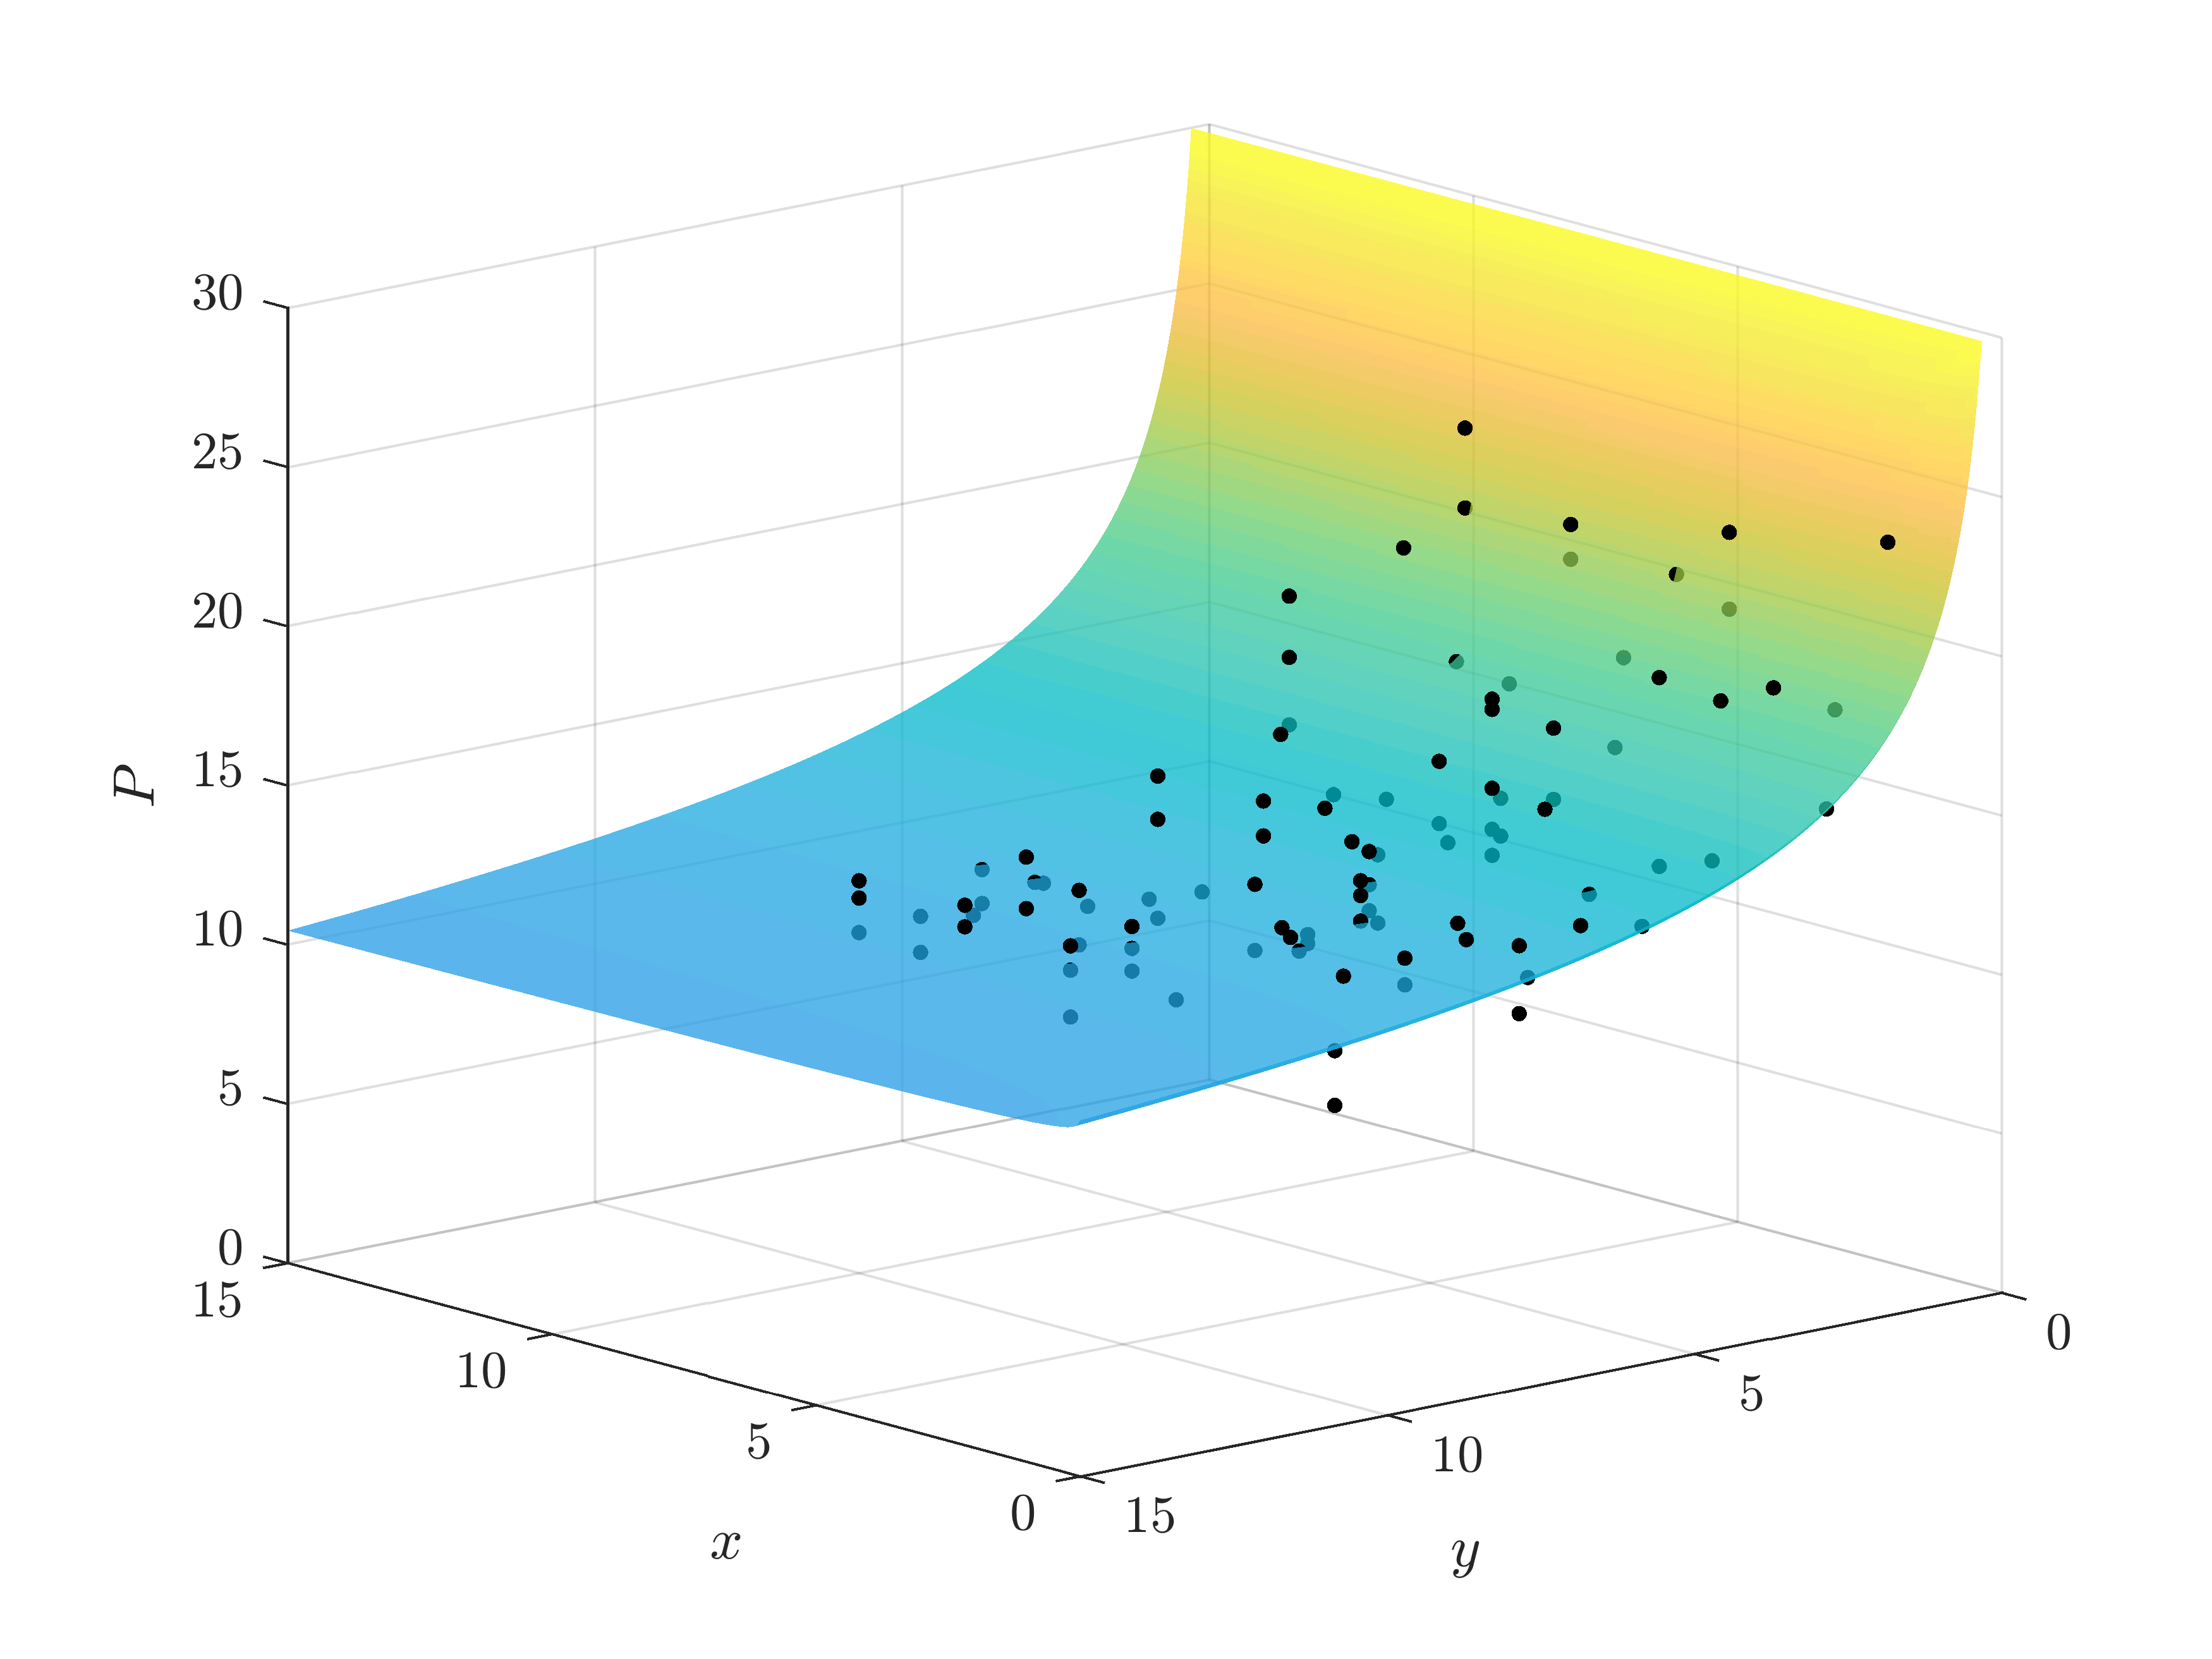
\includegraphics[width=0.6\textwidth]{images/fitprice.png}

Historical prices and fitting surface $p=f(x,y)$.
\end{center}

\end{slide}



\begin{slide}

\question

\begin{problem}%[Unconstrained Optimization]
	A manufacturer of lawn furniture makes two types of chairs, one with a wood frame and the other with an aluminum frame. The wood frame chair costs \$18 per unit to manufacture and aluminum frame chair costs \$10 per unit to manufacture. The company operates in a market where the number of units that can be sold depends on price. It is estimated that in order to sell $x$ units per day of the wood chair and $y$ units per day of the aluminum chair, the selling price cannot exceed $10 + 31x^{-0.5} + 1.3y^{-0.2}$ dollars per unit for the wood chair and $5 + 15y^{-0.4} + 0.8x^{-0.08}$ dollars per unit for the aluminum chair.
\end{problem}


\begin{parts}
	\item We want to maximize the manufacturer's profit. What is the function to maximize?
	\item This is a two-dimensional function, so we need to solve the system
	\begin{align*}
		\frac{\partial f}{\partial x} & = 0 \\[5pt]
		\frac{\partial f}{\partial y} & = 0		
	\end{align*}

	Write down this system.
	\item How can we find the solution?
\end{parts}
	
\end{slide}




\addcontentsline{toc}{subsection}{Newton's Method}


\begin{slide}

\SavedDefinitionRender{Newton1}
\begin{minipage}{0.6\textwidth}
	
\begin{parts}
\setcounter{partsitem}{3}
	\item From the description above, sketch the point $x_1$ on the graph on the right when using Newton's method.
	
	\item What is the formula for $x_1$?
	
\begin{slidesonly}
	\bigskip
\end{slidesonly}
	
	\item Leveraging python.
	\begin{enumerate}
%		\item Go to \url{https://utoronto.syzygy.ca/jupyter}
%		\item Download the file \href{https://raw.githubusercontent.com/bigfatbernie/IBLMathModeling/main/python/chairs_newton.ipynb}{\tt chairs\_newton.ipynb} and import it into the Jupyter Notebook
		\item Clone the file \href{https://utoronto.syzygy.ca/jupyter/user-redirect/git-pull?repo=https://github.com/bigfatbernie/IBLMathModeling&subPath=book/python/chairs_newton.ipynb}{\tt chairs\_newton.ipynb} into your Jupyter Notebook
		\item In the file, introduce the partial derivative functions and an initial guess.
		\item Run the script
	\end{enumerate}
\end{parts}
\end{minipage}
\hfill
	\begin{minipage}{0.35\textwidth}
		\begin{tikzpicture}%[scale=0.65]
		  \draw[-latex] (0,-1.5) -- (0,2.5);
		    \draw[-latex] (-0.25,0) -- (6,0);
		%    \draw[ultra thick, blue, variable=\x, samples=100,domain=0:8] plot ({\x},{(-1.5*sin(180*(\x-4.5)/pi)*(\x-4.5+0.1(\x-4.5)^3-3*(\x-4.5))/4});
		    \draw[ultra thick, blue, variable=\x, samples=100,domain=-0.25:6] plot ({\x},{(-1.5*sin(180*(\x-4.5)/pi)*(\x-4.5)+0.1*(\x-4.5)^3-3*(\x-4.5)-0.2)/5});
		  \draw[dashed, thick] (2,{(-1.5*sin(180*(2-4.5)/pi)*(2-4.5)+0.1*(2-4.5)^3-3*(2-4.5)-0.2)/5}) -- (2,0) node[below] {$x_0$};
		  \draw[ultra thick, green!50!black, fill=green!75!black] (2,{(-1.5*sin(180*(2-4.5)/pi)*(2-4.5)+0.1*(2-4.5)^3-3*(2-4.5)-0.2)/5}) circle (0.1);
		\end{tikzpicture}
	\end{minipage}

\end{slide}


\begin{slide}

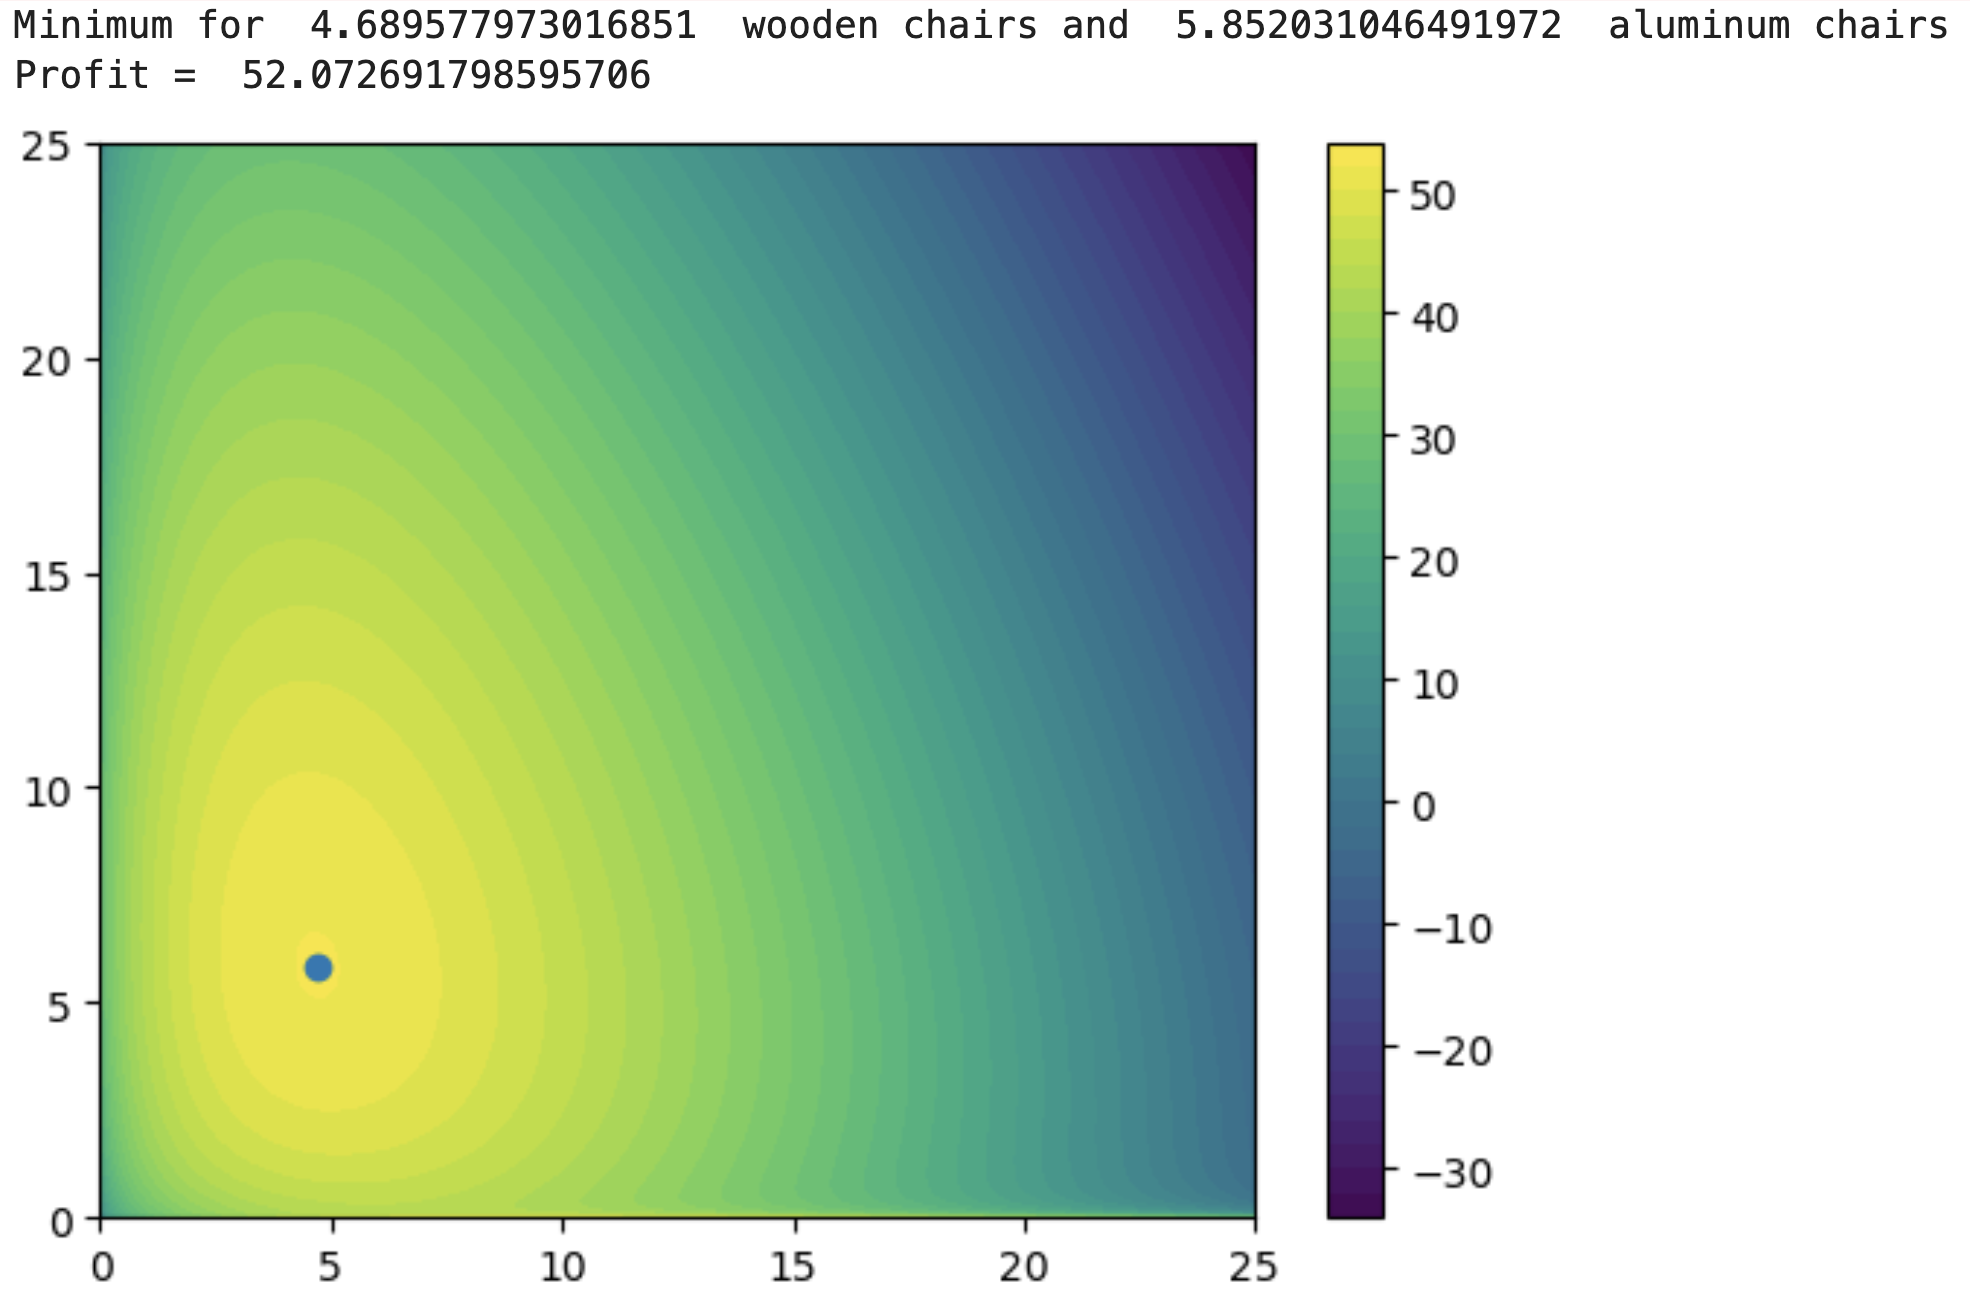
\includegraphics[width=.75\textwidth]{images/chairs-profit.png}
	
\end{slide}

\begin{slide}

\begin{parts}
\setcounter{partsitem}{5}
	\item Leveraging python's minimization tools.
	\begin{enumerate}
%		\item Go to \url{https://utoronto.syzygy.ca/jupyter}
%		\item Download the file \href{https://raw.githubusercontent.com/bigfatbernie/IBLMathModeling/main/python/chairs_fmin.ipynb}{\tt chairs_fmin.ipynb} and import it into Jupyter Notebook
		\item Clone the file \href{https://utoronto.syzygy.ca/jupyter/user-redirect/git-pull?repo=https://github.com/bigfatbernie/IBLMathModeling&subPath=book/python/chairs_fmin.ipynb}{\tt chairs\_fmin.ipynb} into your Jupyter Notebook
		\item In the file, introduce the profit function and an initial guess.
		\item Run the script
	\end{enumerate}
\end{parts}
\end{slide}


\begin{slide}

\question

\begin{problem}%[Unconstrained Optimization]
	A manufacturer of lawn furniture makes two types of chairs, one with a wood frame and the other with an aluminum frame. The wood frame chair costs \$18 per unit to manufacture and aluminum frame chair costs \$10 per unit to manufacture. The company operates in a market where the number of units that can be sold depends on price. It is estimated that in order to sell $x$ units per day of the wood chair and $y$ units per day of the aluminum chair, the selling price cannot exceed $10 + 31x^{-0.5} + 1.3y^{-0.2}$ dollars per unit for the wood chair and $5 + 15y^{-0.4} + 0.8x^{-0.08}$ dollars per unit for the aluminum chair.
\end{problem}


\textbf{Sensitivity}. To compute $p^\star$, you can use \href{https://utoronto.syzygy.ca/jupyter/user-redirect/git-pull?repo=https://github.com/bigfatbernie/IBLMathModeling&subPath=book/python/chairs_sensitivity.ipynb}{\tt chairs_sensitivity.ipynb}.

\begin{parts}
	\item How sensitive is the profit to the parameter $c = 10$ (the production cost of the aluminum chair)
		\[ S(p^\star, c) %= \frac{\partial S}{\partial c} (p^\star,c) \cdot \frac{c}{p^\star(c)} 
			\approx \frac{p^\star(c+h) - p^\star(c)}{h} \cdot \frac{c}{p^\star(c)}?
		\]

	\item How sensitive is the profit to the parameter $b = 0.4$ (the exponent of $y$ in the selling price of the aluminum chair)
		\[ S(p^\star, b) \approx \frac{p^\star(b+h) - p^\star(b)}{h} \cdot \frac{b}{p^\star(b)}?
		\]
\end{parts}

% We already calculated all the terms in these expressions for S except the $p^\star(b+h)$. Those are the only ones we need to calculate.

\begin{solution}
\hspace{-3em}Note that we are using numerical derivatives, since calculating the partial derivatives analytically is usually impossible.	
\end{solution}



\end{slide}






\addcontentsline{toc}{subsection}{Constrained Optimization}


\addcontentsline{toc}{subsubsection}{Lagrange Multipliers}



\begin{slide}

\question

\textbf{Constrained Optimization.} 
How do we solve optimization problems with constraints?

\SavedDefinitionRender{LagrangeMultipliers}


\begin{definition}[Notes:]
\begin{enumerate}
	\item This is a necessary, but not sufficient condition.
	\item To solve the optimization problem, find candidates $x$ that satisfy it, and then pick the best one.
	\begin{itemize}
		\item Points for which $\nabla g_1(x), \ldots, \nabla g_k(x)$ are linearly dependent should also be candidates.
	\end{itemize}
	\item \eqref{LM} $\Leftrightarrow \nabla f(x^\star) \in {\rm span}\Big\{\nabla g_1(x), \ldots, \nabla g_k(x)\Big\}$.
	\item The ``optimal'' values for $\lambda_1, \ldots, \lambda_k$ give important insights on the problem, as we will see -- don't ignore them!
\end{enumerate}
\end{definition}

\end{slide}





\begin{slide}
	
\begin{problem}[Example]
Consider the problem:
\begin{itemize}
	\item Maximize $x+y$ \quad such that $x^2+y^2 = 1$.
\end{itemize}
\end{problem}

\begin{center}
	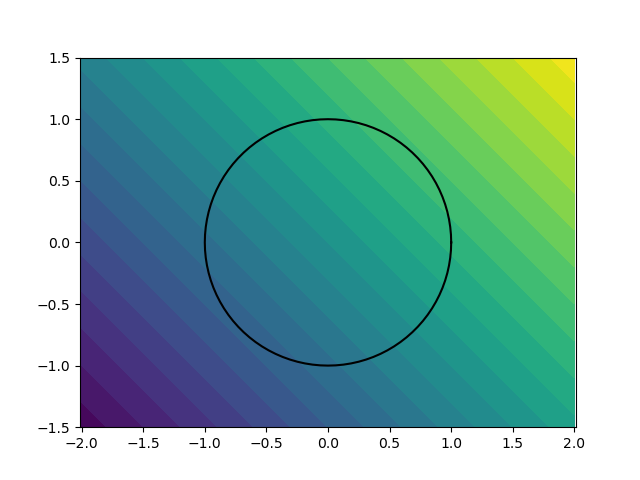
\includegraphics[width=.4\textwidth]{images/LagrangeMultipliers-ex.png}
\end{center}

\begin{parts}
	\item Use Lagrange Multipliers to find the maximum (and the minimum).

	\item If the constraint was $x^2+y^2=c$, then what is:
	\begin{enumerate}
		\item the maximizer point $(x^\star,y^\star)$?
		\item the Lagrange multiplier $\lambda^\star$?
		\item the maximum $f(x^\star,y^\star)$?
	\end{enumerate}
	
	\item Compare $\lambda^\star$ with $\dfrac{\partial f(x^\star,y^\star)}{\partial c}$.
	
	\item Based on this relation, give an interpretation for the Lagrange Multiplier.
	
\end{parts}

\end{slide}


\begin{solution}
\begin{slide}

\begin{parts}
	\item 
	\begin{align*}
		\nabla f & = \mat{1\\1}  
			\quad \text{ and } \quad \nabla g = \mat{2x\\2y} \\
		\\
		\mat{1\\1} & = \lambda \mat{2x \\ 2y} \quad \Leftrightarrow \quad 
			\begin{cases}
				1 & = 2\lambda x \\
				1 & = 2\lambda y \\
				1 & = x^2 + y^2	
			\end{cases}
			\\
		1 & = \frac{1}{2 \lambda^2} \quad \Leftrightarrow\quad 
			\lambda = \pm\frac{1}{\sqrt{2}}\\
		x & = y = \pm \frac{1}{\sqrt{2}}
	\end{align*}
	
	\item $x^\star=y^\star= \frac{\sqrt{c}}{\sqrt{2}}$ \quad and \quad $\lambda^\star = \frac{1}{\sqrt{2c}}$
		 
		 $\max = x^\star+y^\star=\sqrt{2c}$
		
	\item $\dfrac{\partial f(x^\star,y^\star)}{\partial c}
			= \dfrac{\sqrt{2}}{2\sqrt{c}} = \lambda^\star$

	\item This means that if the constraint increased from $1$ to $1 + \Delta = 1.1$, 	then we would expect the maximum to increase by approximately $\Delta \lambda^\star = \frac{\Delta}{\sqrt{2}} \approx 0.07$.
		
		Indeed, $\Delta f = \sqrt{2.2}-\sqrt{2} \approx 0.069$.

\end{parts}
	
\end{slide}	
\end{solution}


%\begin{solution}
%\begin{slide}
%
%We obtain the following equations:
%\begin{align*}
%	\nabla f & = \mat{1\\1} \\	
%	\nabla g & = \mat{2x\\2y} \\
%	\\
%	\mat{1\\1} & = \lambda \mat{2x \\ 2y} \\
%	\\
%	1 & = 2\lambda x \\
%	1 & = 2\lambda y \\
%	1 & = x^2 + y^2 \\
%	\\
%	1 & = \frac{1}{2 \lambda^2} \\
%	\lambda & = \pm\frac{1}{\sqrt{2}}\\
%	x & = y = \pm \frac{1}{\sqrt{2}}
%\end{align*}
%		
%\end{slide}
%\end{solution}









\begin{slide}

\question

\textbf{Define the problem.}

\begin{problem}
The production side of the electrical power grid\footnote{This example is based on \href{https://sces.phys.utk.edu/~moreo/mm08/method_HLi.pdf}{Huijuan Li in `Lagrange Multipliers and their Applications'}.} consists of hundreds or thousands of power plants that vary in fuel sources (coal, nuclear, hydroelectric, solar, wind, stored energy in the batteries of electric vehicles, etc.) and characteristics (age, efficiency, automated, etc.). 

How can the power consumption load be allocated to these plants to minimize cost?
\end{problem}


\textbf{Make Assumptions.}

\begin{itemize}
	\item Each power plant is summarized by a cost curve which tells how much a given load costs. Generally, the cost per unit time per unit load of operating a power plant is a concave function of load as in the figure below: small and large loads are expensive.
	\item For simplicity, we will approximate these quadratics by a linear function with one parameter: the cost per unit time per unit load is $c(x) =ax+1$, so the cost rate function has the form $f(x)=(ax+1)x = ax^2+x$.
	
	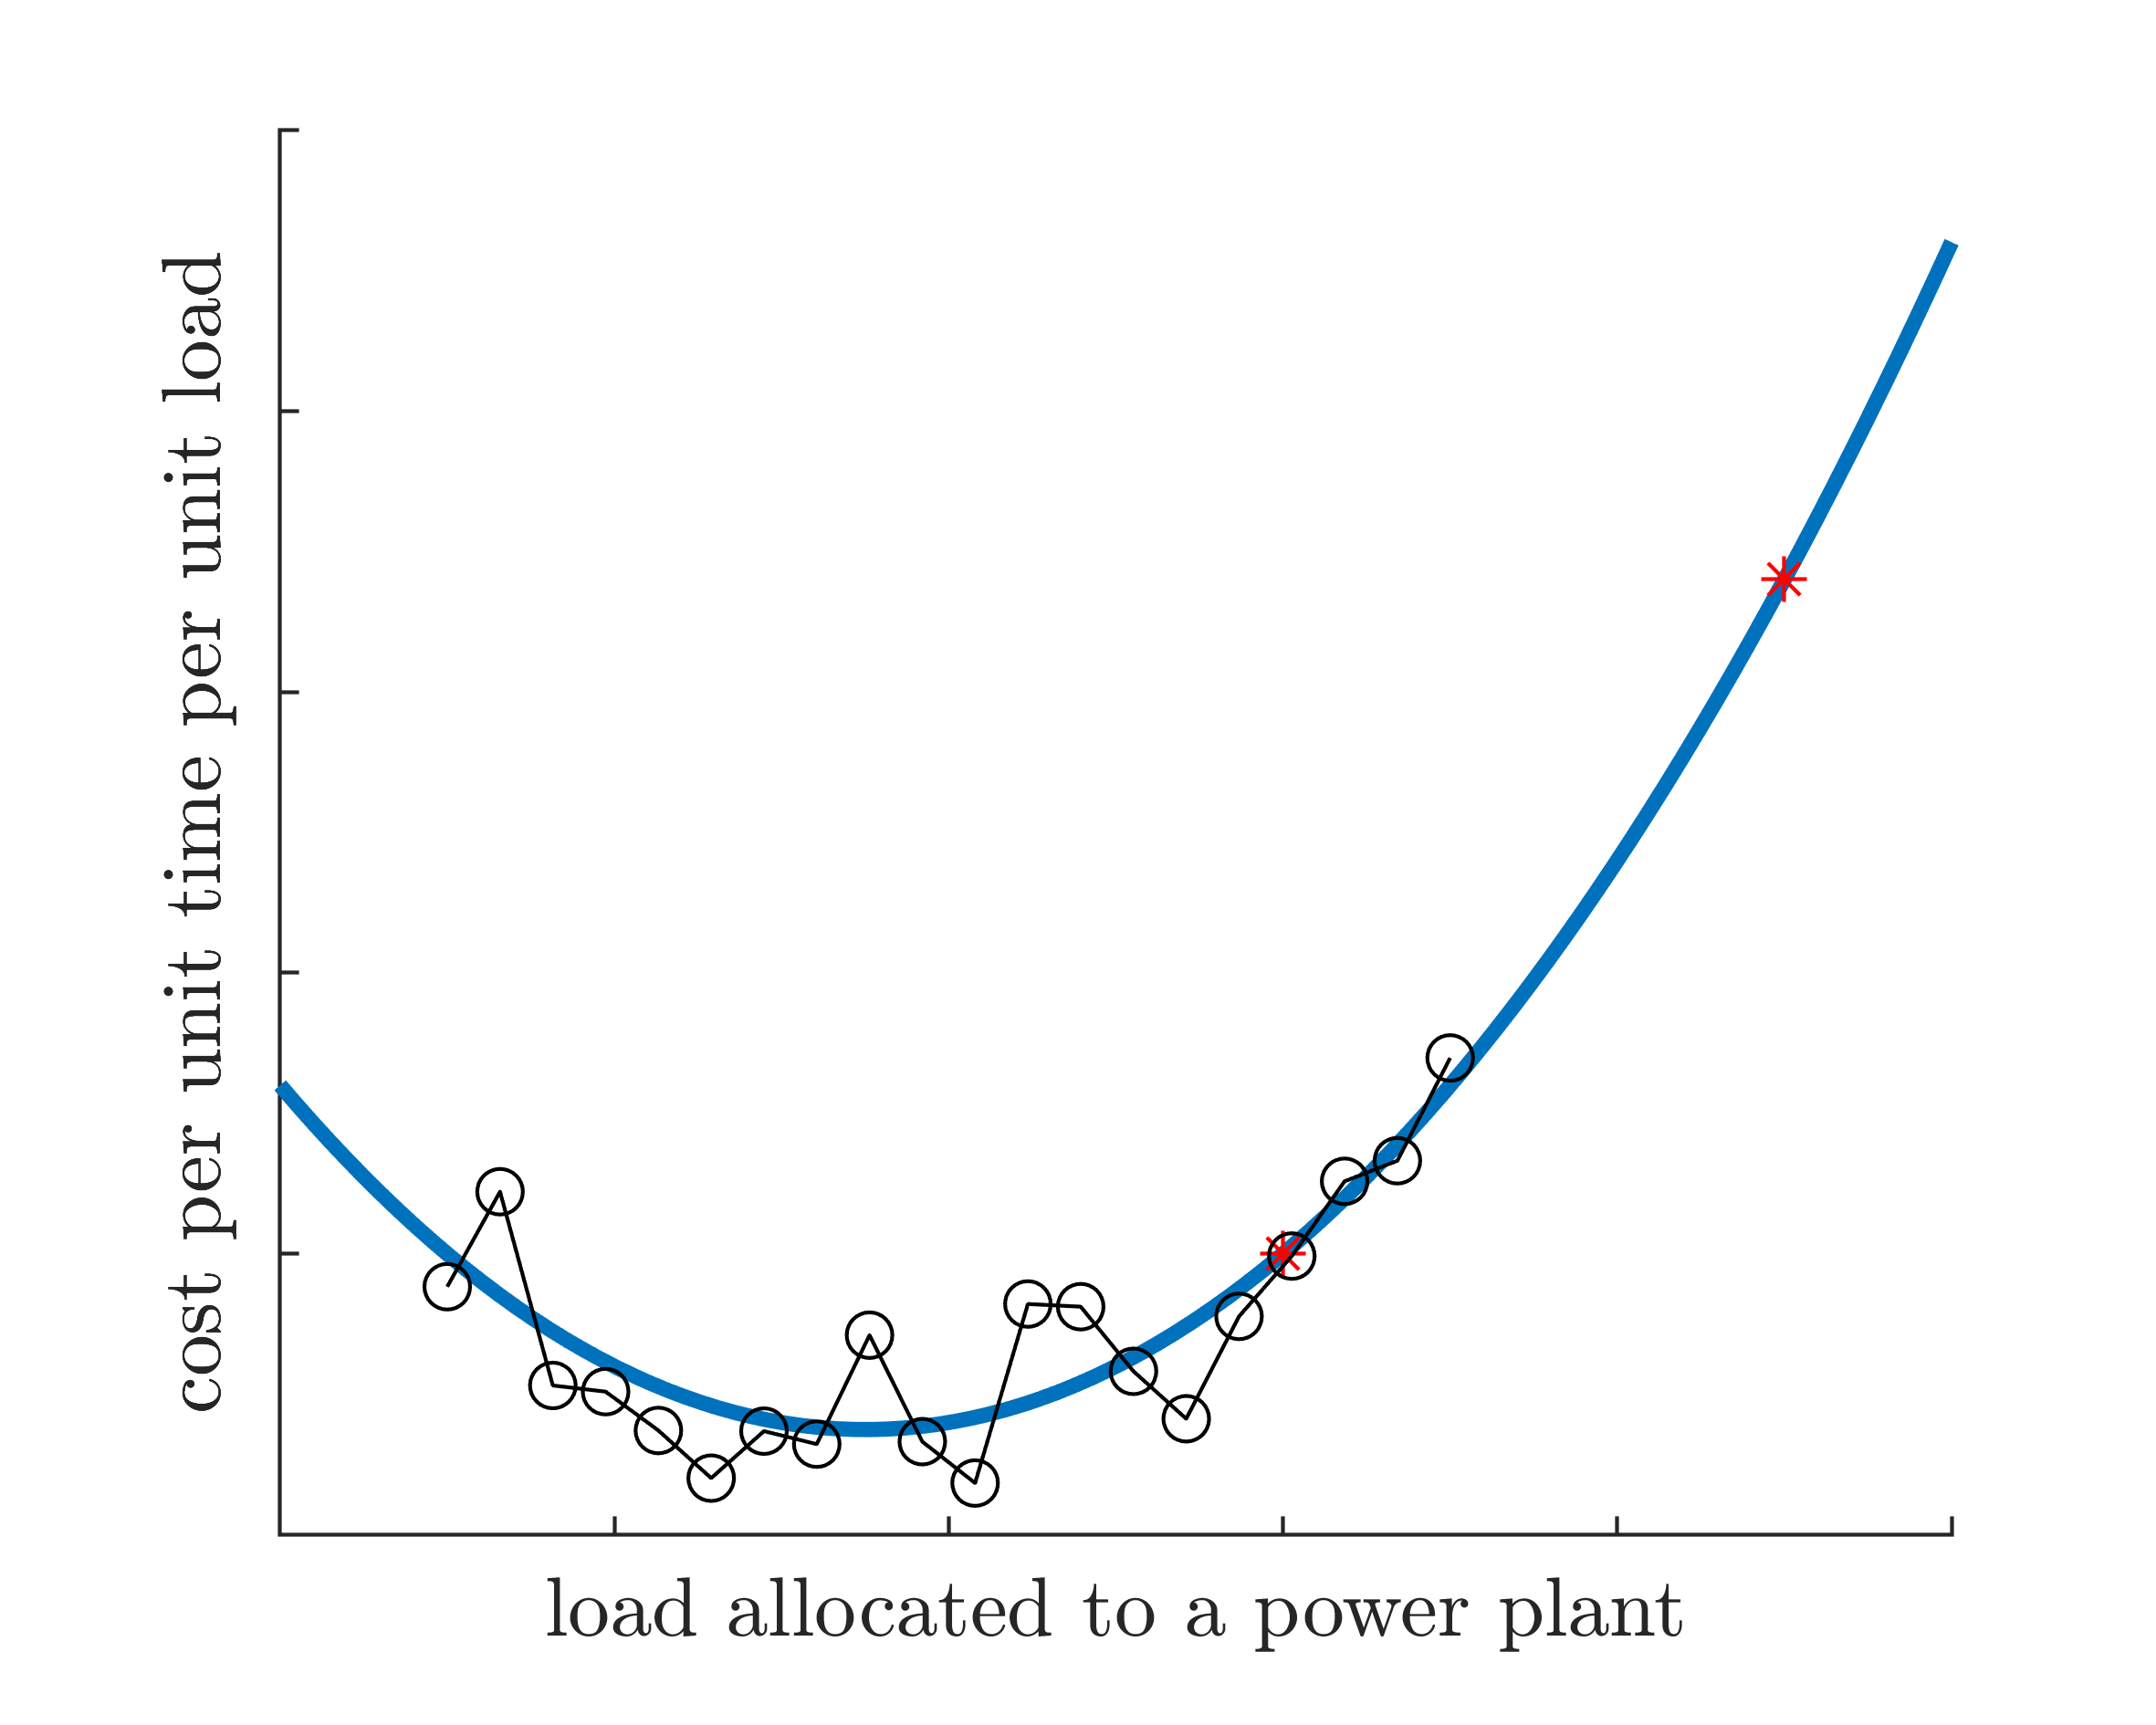
\includegraphics[width=.4\textwidth]{images/concavecost.png} 
	
	\item $N=$ number of power plants
	\item $x_i=$ load assigned to power plant $i$ (in MW)
	\item $X=$ total load (in MW)({In Toronto the average total load is 2500 MW.}).
	\item $C=$ cost rate of power generation (in \$/h)
	\item $f_i(x_i)=$ cost rate function for power plant $i$ (in \$/h)
	

\end{itemize}

	
\end{slide}


\begin{slide}

\textbf{Build a model.}

\begin{parts}
	\item Find an equation relating $X$ and $x_i$.
	\item Find a formula for $C$.
	\item Formulate the problem we want to solve.
	

\begin{slidesonly}
	\bigskip
\end{slidesonly}

\hspace{-2em}
\textbf{Assess the model.}

\hspace{-2em}
	We are going to assume the following:
	\begin{itemize}
		\item Three power plants identified with the parameters:
		\begin{itemize}
			\item $a_1 = 0.0625 $
			\item $a_2 = 0.0125 $
			\item $a_3 = 0.0250 $
		\end{itemize}
		\item The total load is 925 MW
	\end{itemize}


	\item Solve the problem.

\begin{slidesonly}
	\vspace{5cm}
\end{slidesonly}

\hspace{-2em}
\textbf{Report the results.}

	\item What is the interpretation of $\lambda^\star$ the ``optimal'' Lagrange multiplier?
	\item What is the sensitivity of the cost with respect to the parameters $a_i$ and $X$? What does that mean about the model?
		
\end{parts}
	
\end{slide}


\begin{solution}
\begin{slide}

\begin{parts}
\setcounter{partsitem}{2}
	\item 	
		\begin{tabular}[t]{ll}
			Objective: 	& $\displaystyle \min \quad \sum_{i=1}^3 a_i x_i^2 + x_i$ \\
			Constraint: & $\displaystyle \sum_{i=1}^3 x_i = X$
		\end{tabular}

	\item Define:
		\begin{align*}
			C(\vec{x}) & = \sum_{i=1}^3 a_i x_i^2 + x_i \\
			g(\vec{x}) & = \sum_{i=1}^3 x_i = X
		\end{align*}
		
		So we have
		\[
			\nabla C (\vec{x}) 
				= \mat{2a_1 x_1 + 1\\2a_2 x_2 + 1\\2a_3 x_3 + 1} 
				= \lambda	\nabla g (\vec{x}) 
				= \lambda \mat{1\\1\\1}
		\]
		
		Which can be written as
		\[ \matc{2a_1 & 0 & 0 & -1\\0 & 2a_2 & 0 & -1\\0 & 0 & 2a_3 & -1 \\ 1 & 1 & 1 & 0} \mat{x_1\\x_2\\x_3\\\lambda} = \mat{-1\\-1\\-1\\ X}
		\]
		
		And we get the unique solution:
		\begin{itemize}
			\item $x_1 = 112$ MW
			\item $x_2 = 560$ MW
			\item $x_3 = 280$ MW
			\item $\lambda = \$15$ /h/MW (shadow cost)
		\end{itemize}
		
		We used: \href{https://utoronto.syzygy.ca/jupyter/user-redirect/git-pull?repo=https://github.com/bigfatbernie/IBLMathModeling&subPath=book/python/power-plants.ipynb}{\tt power-plants.ipynb}
		
		\item If we reduce the total load ($X$) by 1 MW, it would approximately reduce the total cost of operating the three power plants by \$15/h.
		
		So the operator of the power plants should be willing to pay consumers who pump electricity back to the grid up to \$15/h for each megawatt.

		\item 	\begin{itemize}
			\item $S(C,X) \approx 1.875$
			\item $S(C,a_1) \approx 0.000015$
			\item $S(C,a_2) \approx 0.00017$
			\item $S(C,a_3) \approx 0.00007$
		\end{itemize}


	
\end{parts}
	
\end{slide}
	
\end{solution}


\begin{slide}

\question

\textbf{Robustness.} 

\begin{parts}
	\item The parameter $X$ varies significantly (regularly by over 50\% in a day), so understanding it is very important.

\begin{center}
	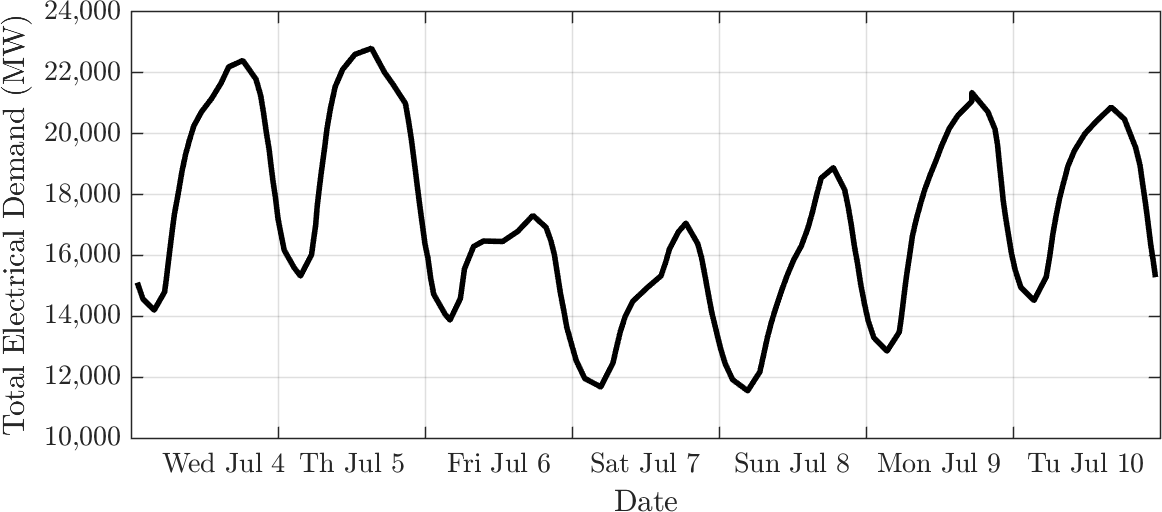
\includegraphics[width=0.4\textwidth]{images/energydemand.png}
\end{center}
	

It is crucial to understand how the optimal cost and loads change with $X$.


	\item Is the quadratic model for $f_i$ good? You can try different functions.
	\item Should there be other constraints on $x_i$? We only imposed $x_i>0$, but we probably should impose upper bounds too.
	\item What about transportation costs? There can be losses of up to 20\% on high-tension transmission lines.
	\item We have a static model, where the power plants operate always at the same load. We might want to consider a dynamic optimization model.
\end{parts}



\end{slide}





\addcontentsline{toc}{subsection}{Linear Programming}


\begin{slide}
\question

\begin{problem}[Linear Programming\footnote{based on a problem from Meerschaert's `Mathematical Modeling'.}]
	A family farm has 1250 hectares\footnote{1 hectare $=1$ ha $=$ 10\,000 m$^2$.}  of land for planting. Possible crops that they could plant are corn, wheat, and oats. There are 400 hectare-m (a volume) of water available for irrigation and 600 hours of labour per week available. The requirements and expected yields are shown below.
	
	
	\begin{center}
	\small
	\begin{tabular}{l|c|c|c}
	%\hline
	& corn & wheat & oats \\ \hline
	irrigation (ha-m / ha) & 1.0 & 0.3 & 0.5 \\ \hline
	labour (person-h / week / ha) & 1.6 & 0.4 & 0.6 \\ \hline
	yield (\$/ha) & 1400 & 420 & 700 \\ %\hline
	\end{tabular}
	\end{center}
	
	We want to maximize the total yield.
\end{problem}

Introduce the following variables:
\begin{itemize}
	\item $x_i= $ hectares planted of $i=1$ corn, $i=2$ wheat, $i=3$ oats
	\item $w=$ the total irrigation used in ha-m
	\item $\ell=$ the total labour used in person-h / week
	\item $a=$ the total area planted in hectares
	\item $y=$ the total yield in \$
\end{itemize}

\begin{parts}
	\item Find expressions for $w, \ell, a, y$
	\item What are the constraints on the variables defined?	
	\item Formulate the optimization problem we want to solve in standard linear programming form:
	\begin{center}
		\begin{tabular}{lc}
		Objective: 		& max \ $\vec{c}^T \vec{x}$ \\
		\multirow{2}{*}{Constraints:} 	& $A \vec{x} \leq \vec{b}$ \\
						& $\vec{x} \geq \vec{0}$
		\end{tabular}
	\end{center}
	\item Use \href{https://utoronto.syzygy.ca/jupyter/user-redirect/git-pull?repo=https://github.com/bigfatbernie/IBLMathModeling&subPath=book/python/farm-linearprog.ipynb}{\tt farm-linearprog.ipynb} to find the solution.

\end{parts}

\end{slide}


\begin{solution}
\begin{slide}
\begin{parts}
	\item
		\begin{itemize}
			\item $w = 1x_1 + 0.3x_2 + 0.5 x_3$
			\item $\ell = 1.6 x_1 + 0.4 x_2 + 0.6 x_3$
			\item $\displaystyle a = \sum_{i=1}^3 x_i$
			\item $y = 1400 x_1 + 420 x_2 + 700 x_3$
		\end{itemize}
		
	\item 
		\begin{itemize}
			\item $x_i \geq 0$
			\item $w \leq 400$
			\item $\ell \leq 600$
			\item $a \leq 1250$
		\end{itemize}
	\item 	\begin{tabular}[t]{lc}
				Objective: 						& max \ $\mat{1400 & 420 & 750} \vec{x}$ \\
				\multirow{2}{*}{Constraints:} 	& $\mat{1 & 0.3 & 0.5\\1.6 & 0.4 & 0.6\\1 & 1 & 1} \vec{x} \leq \mat{400\\600\\1250}$ \\
							& $\vec{x} \geq \vec{0}$
			\end{tabular}
\end{parts}
\end{slide}
\end{solution}

\begin{slide}

We ran the same model with the Wheat Yield ranging from \$400/ha to \$440/ha and obtained the following graphs.
\begin{center}
	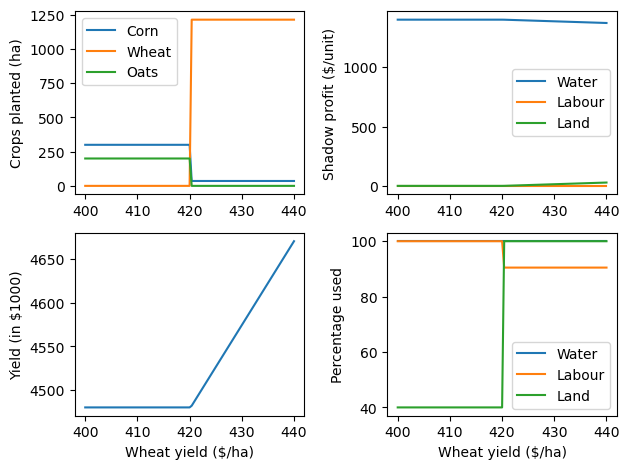
\includegraphics[width=.5\textwidth]{images/farm-linearprog.png}
\end{center}

\begin{parts}
	\setcounter{partsitem}{4}
	\item Interpret the results and the shadow profit ($-$ shadow cost).
\end{parts}
\end{slide}




\begin{slide}
\question

\begin{problem}[Modified farming problem]
We modify the original optimal farming problem to include the notion of plots. The 1250 hectares farm is broken down into 5 plots of 240 hectares each and one 50 hectare plot. For convenience, the farmers want to plot only one crop on each plot. As before, 400 ha-m of water and 600 hours of labour are available. 
The requirements and expected yields are shown below.
	
	\begin{center}
	\small
	\begin{tabular}{l|c|c|c}
	%\hline
	& corn & wheat & oats \\ \hline
	irrigation (ha-m / ha) & 1.0 & 0.3 & 0.5 \\ \hline
	labour (person-h / week / ha) & 1.6 & 0.4 & 0.6 \\ \hline
	yield (\$/ha) & 1400 & 420 & 700 \\ %\hline
	\end{tabular}
	\end{center}
	
	We want to maximize the total yield.
\end{problem}

Introduce the variables:
\begin{itemize}
	\item $x_1, x_2, x_3$ are the number of large plots of corn, wheat, and oats respectively;
	\item $x_4, x_5, x_6$ are the number of small plots of corn, wheat, and oats respectively.
\end{itemize}

\begin{parts}
	\item Set up and solve the problem.
	\item Interpret the results.
\end{parts}

	
\end{slide}


\begin{slide}

\question

\begin{problem}[Ice Cream\footnote{Based on an example from Kamien and Schwartz's `Dynamic Optimization'}]

Suppose a manufacturing company receives an order for $B$ units to be delivered at time $T$, e.g. Sobeys has placed an order for $B = 100$ pallets of Chapman's vanilla ice-cream for a promotion starting in $T = 10$ days.

Chapman's Ice Cream must decide when to produce their tasty product. They don't want to produce it early since they will have to pay to keep it frozen until the order is due. They also do not want to produce it the day before it is due since running the production line fast might have a large cost. %For example, running the machines quickly might have more waste or might produce more and expansive wear-and-tear on the machines.
\end{problem}

Let $x(t)$ be the inventory at time $t$ and suppose that $x(0)=0$ and to fill the order we need $x(T)=B$ (boundary conditions).

\begin{parts}
	\item Let us divide the time interval $[0,T]$ into $N$ ``chunks''. What is the length $\Delta t$ of each?
	\item Let $\Delta x_n$ be the number of units produced during the $n^{\rm th}$ time interval. Find a formula relating $\Delta x_n$ with $x(t)$. Find an equation relating $\Delta x_n$ with $B$.
	\item We need to consider the cost of storing the produced units in inventory: assume that each unit has a cost of $c_2$ per unit time. What is the total inventory cost?
	\item We want to model the fact that running machines faster is more costly. What is a model for the cost of producing $\Delta x_n$ units during a time interval of length $\Delta t$ that quantifies this?
	\item What is the total production cost? 
	\item What is the total cost?
	\item What are the constraints for the variables?
	\item Approximate the solution.
\end{parts}
\end{slide}


\begin{solution}
\begin{slide}

\begin{parts}

\item Let us break the time interval $[0,T]$ into $\Delta t = T/N$ ``chunks'' and consider $t_n=n \Delta t$. We need to decide how many units $\Delta x_n$ to produce at each time interval.

\item We then have:
\begin{itemize}
	\item $x(t_{n+1})) = x(t_n) + \Delta x_n$
	\item $\Delta x_1 + \cdots + \Delta x_N = B$
\end{itemize}

\item We need to consider the cost of storing the produced units in inventory: assume that each unit has a cost of $c_2$ per unit time:
\begin{itemize}
	\item Inventory Cost $\displaystyle = \sum_{n=1}^N \Delta x_n (T-t_n) c_2$
\end{itemize}

\item If the production cost was: $\displaystyle\sum_{n=1}^N c \Delta x_n$, then $c=$ the cost of producing 1 unit in $\Delta t$ time.

If this is constant, then there is no penalty in running the machines faster, so we need to consider $c$ that is not constant and depends on $\Delta x_n$: we make the modelling assumption $c = c_1 \frac{\Delta x_n}{\Delta t}$, so that $c$ is proportional to the rate of production.
We get
\begin{itemize}
	\item Production Cost $\displaystyle = \sum_{n=1}^N  \frac{\Delta x_n^2}{\Delta t} c_1	$
\end{itemize}

\item So the total cost is
\begin{itemize}
	\item Total Cost $\displaystyle = \sum_{n=1}^N \bigg[ \Delta x_n^2 c_1 + \Delta x_n (N-n) c_2 \bigg]$
\end{itemize}

\item The constraints are
\begin{itemize}
	\item $\Delta x_1 + \cdots + \Delta x_N = B$
	\item $\Delta x_n \geq 0$
\end{itemize}

	
\item The solution is here: \href{https://utoronto.syzygy.ca/jupyter/user-redirect/git-pull?repo=https://github.com/bigfatbernie/IBLMathModeling&subPath=book/python/IceCream.ipynb}{\tt IceCream.ipynb}


\end{parts}

\end{slide}
\end{solution}



\addcontentsline{toc}{subsection}{Calculus of Variations}



\begin{slide}
\question \label{q:cv}

In the previous problem, instead of modelling it using \textbf{discrete time}, we can model it using \textbf{continuous time}.

Then, we have the following:
\begin{itemize}
	\item $\frac{dx}{dt}(t) = $ units produced per unit time (at time t)
	\item Inventory cost $\displaystyle= \int_0^T c_2 \frac{dx}{dt}(t) (T-t) \, dt = \int_0^T c_2 x(t) dt$ \hfill (why?)
	\item Production cost $\displaystyle= \int_0^T c_1 \left(\frac{dx}{dt}\right)^2 \, dt$
		\hfill (why?)
\end{itemize}
We can formulate the problem as
\begin{problem}
\begin{tabular}[t]{lc}
	Objective: 						& min \ $\displaystyle\int_0^T c_1 \big(x'(t)\big)^2 + c_2 x(t) ~dt$ \\[10pt]
	\multirow{2}{*}{Constraints:} 	& $x(0)=0$ and $x(T)=B$ \\
				& $x'(t) \geq 0$
\end{tabular}

The goal here is to find a function $x(t)$. This is a problem in \textbf{Calculus of Variations}.
\end{problem}


\end{slide}



\addcontentsline{toc}{subsubsection}{Euler-Lagrange Equation}


\begin{slide}
\question

\begin{problem}[Euler-Lagrange Equation]

We want to find a function $x: [t_0,t_1] \to \R$ that minimizes the functional:
\[ \min \int_{t_0}^{t_1} F \big(t, x(t), x'(t) \big) ~dt \]
and $x(t_0)=x_0$ and $x(t_1)=x_1$.
\end{problem}

When we want to find a minimizer of a function, \textsl{we set the derivative to zero}.



\begin{parts}
	\item The definition of derivative for a real function is
	\[ f'(x) = \lim_{\varepsilon \to 0} \frac{f(x+\varepsilon)-f(x)}{\varepsilon} \]
	
	We only have one direction for $\varepsilon$, so this limit suffices. For a function of multiple variables, we introduced the notion of partial derivative:
	\[ \frac{\partial f}{\partial x_i}(\vec{x}) = \lim_{\varepsilon \to 0} \frac{f(\vec{x}+\varepsilon \vec{e}_i)-f(\vec{x})}{\varepsilon} \]
	
	Our case is similar, but instead of having vectors as inputs, our inputs are functions $x(t)$, so our definition must be adapted to:
	\begin{itemize}
		\item Let $y(t) = x(t) + \varepsilon v(t)$
	\end{itemize}	
	
	What are conditions on $v(t)$ that guarantee that $y(t)$ is an admissible function for the problem formulated in the blue box above?
	
	\item Let $\displaystyle g(\varepsilon) = \int_{t_0}^{t_1} F\big( t, y(t), y'(t) \big) ~dt$. Expand the formula for $g(\varepsilon)$.

	\item Expand $g'(0)$.

	\item Set $g'(0)=0$ and solve.
	
	\textit{Hint: If $\int_a^b f(t) v(t) ~dt=0$ for every function $v(t)$ satisfying $v(a)=v(b)=0$, then $f(t)=0$ for all $t \in (a,b)$.}

\end{parts}
\end{slide}


\begin{slide}
	
\SavedDefinitionRender{EulerLagrange}

\question

We will look back to \textbf{Exercise \ref{q:cv}}.

\begin{parts}
	\item Use the Euler-Lagrange Equation to obtain a Differential equation for $x(t)$.
		
	\item Solve the differential equation with the boundary conditions.
		
	\item We required $x'(t) \geq 0$. Does this solution satisfy this condition?
	
	\item To get a solution that satisfies $x'\geq 0$, we need to consider a solution that doesn't produce any units for a while: 
	\[ x(t) = \begin{cases}
 			0 & \text{ if } t < t_1 \\
 			z(t) & \text{ if } t_1 \leq t \leq T
	 \end{cases}
	 \]
	 
	 What is $t_1$ and what is the function $z(t)$?	
	
	\item If we add a constraint $x'(t) \leq M$, how would that modify the solution? What does this restriction mean in the ice-cream context?
	
\end{parts}
\end{slide}



\begin{solution}
\begin{slide}
\begin{parts}

	\item 
		\begin{align*}
			\frac{\partial F}{\partial x} & = c_2 \\
			\frac{\partial F}{\partial x'} & = c_1 2x'(t) \\
			\frac{d}{dt} \frac{\partial F}{\partial x'} & = 2 c_1 x''(t)
		\end{align*}

		So the Euler-Lagrange equation yields $x''(t) = \frac{c_2}{2c_1}$.
		
	\item 		The general solution of the ODE is: 
			$x(t) = \frac{c_2}{4c_1} t^2 + v_0 t + x_0$
			
		Using the boundary conditions we get:
			\[x(t) = \frac{c_2}{4c_1} t^2 + \frac{4c_1 B-c_2 T^2}{4c_1 T} t\]

	\item 		If $B < \frac{c_2 T^2}{4c_1}$, then $x'$ can be negative at the beginning:
		\begin{align*}
			x'(t) \leq 0 	
				& \Leftrightarrow \frac{c_2}{2c_1} t + \frac{4c_1 B-c_2 T^2}{4c_1 T} \leq 0 \\
				& \Leftrightarrow t \leq \frac{c_2 T^2 - 4c_1 B}{c_2T}	
		\end{align*}
		
		This only happens for small values of $B$. Intuitively, this means that since the order is small, the producer would be better off by selling more of their product to save on inventory (inventory cost becomes negative) and produce the required order later.


	
\end{parts}

\end{slide}	



\begin{slide}
\begin{parts}
	\setcounter{partsitem}{3}

	\item The solution is is decreasing when $c_2 T^2 - 4c_1 B > 0$, so to make sure that this doesn't happen for the new solution, we choose $t_1$ such that $c_2 (T-t_1)^2 - 4c_1 B=0$:
		\[ t_1 = T - \sqrt{ \frac{4c_1 B}{c_2}} \]
	
	The function $z(t)$ is the optimal function $x(t)$ just translated by $t_1$ and with $T \to T-t_1$:
		\[ 
			z(t) = \frac{c_2}{4c_1} (t-t_1)^2 + \frac{4c_1 B-c_2 (T-t_1)^2}{T-t_1} (t-t_1)
		\]

	\url{https://www.desmos.com/calculator/ny2frmc2ov}
	
	\item If $B$ is not too large: $B\leq MT-\frac{c_{2}}{4c_{1}}T^{2}$, then the original solution holds.
		
		If $B$ is too large, then we have too many units to produce in the time provided, so we would need to produce as many as we could ($x'(t)=M$) at the end to be able to complete the order. 
		Before that time, we could produce at the optimal rate.

		\url{https://www.desmos.com/calculator/2rfh1w2a7a}
	
\end{parts}
\end{slide}
\end{solution}










%%%%%%%%%%%%%%%%%%%%%%%%%%%%%%%%%%%%%%%%%%%%%%%%%%%%%
%
%
%  	DYNAMICAL MODELS - ODEs, Systems of ODEs, Bifurcation, PDEs, 
%
%
%%%%%%%%%%%%%%%%%%%%%%%%%%%%%%%%%%%%%%%%%%%%%%%%%%%%%

\phantomsection
\addcontentsline{toc}{section}{Dynamical Models}\label{sec:dynamical}

%%%%%%%%%%%%%%%%%%%%%%%%%%%%%%%%%%%%%%%%%%%%%%%%%%%%%
%
%
%  	DYNAMICAL MODELS - ODEs, Systems of ODEs, Bifurcation, PDEs, 
%
%
%%%%%%%%%%%%%%%%%%%%%%%%%%%%%%%%%%%%%%%%%%%%%%%%%%%%%

\begin{slide}
\question

\begin{slidesonly}
	\vspace{3cm}
\end{slidesonly}

\begin{center}
\Huge 
\textcolor{LimeGreen}{Dynamical Models}
\end{center}

	
\end{slide}








%
%\begin{slide}
%
%\question
%	The tree model
%	\begin{align*}
%		H'(t) &= 0.3\cdot A(t)-b\cdot H(t)\\
%		A'(t) &= -0.3\cdot (H(t))^2 + A(t)
%	\end{align*}
%	was based on the premises
%	\begin{itemize}[leftmargin=3em]
%		\item[ $P_{\text{height 1}}$] CO$_2$ is absorbed by the leaves and turned directly into trunk height.
%		\item[ $P_{\text{height 2}}$] The tree is in a swamp and constantly sinks at a speed proportional to its height.
%		\item[ $P_{\text{leaves 1}}$] Leaves grow proportionally to the energy available.
%		\item[ $P_{\text{energy 1}}$] The tree gains energy from the sun proportionally to the leaf area.
%		\item[ $P_{\text{energy 2}}$] The tree loses energy proportionally to the square of its height.
%	\end{itemize}
%
%	\begin{parts}
%		\item How are the premises expressed in the differential equations?
%		\item What does the parameter $b$ represent (in the real world)?
%
%		\item 
%	\end{parts}
%	
%\end{slide}
%


\addcontentsline{toc}{subsection}{Modelling with ODEs}


\begin{slide}

\question

\begin{center}
	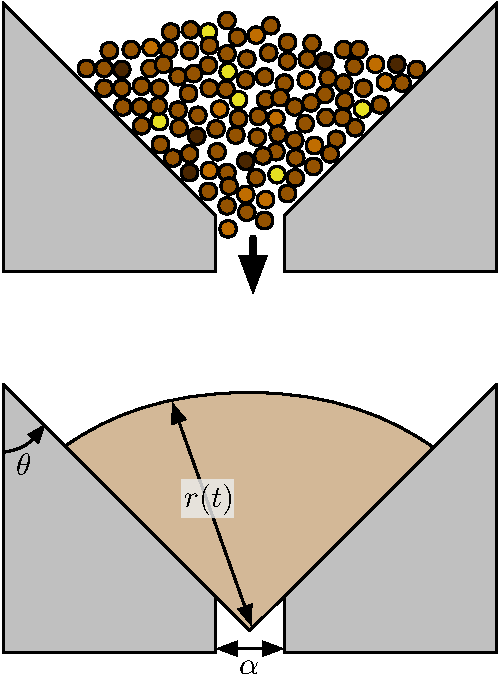
\includegraphics[width=145pt]{images/stadium.pdf}
\end{center}

	The following ordinary differential equation models a crowd leaving a stadium through an exit
	\[
	2 \theta r \frac{dr}{dt_{}} = - k \alpha \sqrt{r}
	\]
	
\begin{slidesonly}
	\bigskip
\end{slidesonly}

	
	based on the premise \\[-20pt]
	\begin{itemize}
		\item[(TL)]	Torricelli's Law: The area of the region occupied by the crowd decreases proportionally to the width of the exit times the square root of its radius. %\\[-20pt]
	\end{itemize}

	\begin{parts}
		\item How is the premise expressed in the differential equation?
		\item Sketch a slope field for this model

			\url{https://www.desmos.com/calculator/lxb4g6cuiz}

		and use it to study how the time it would take to evacuate that section depends on the parameters.
		
		\item Using Euler's method, estimate how long it would take to evacuate a stadium with $\alpha=k=1$, $\theta=\frac{\pi}{5}$ and $r(0)=2$.
		
%		\url{https://www.desmos.com/calculator/2dfs5s1axi}
\end{parts}

\end{slide}


\begin{slide}

\question

\begin{center}
	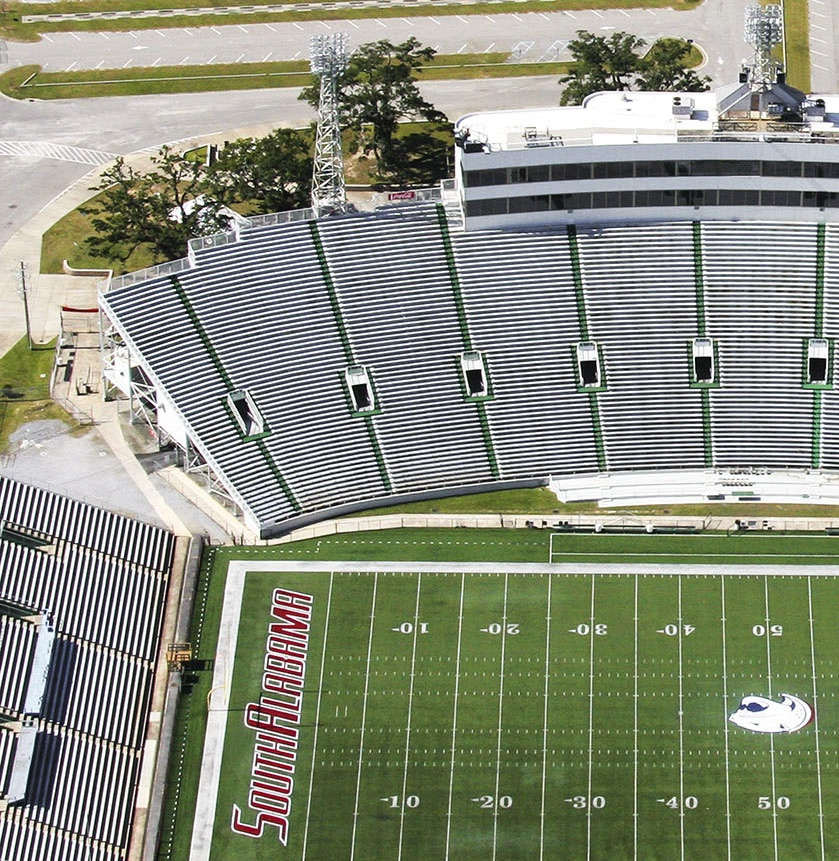
\includegraphics[width=.4\textwidth]{images/Ladd_Stadium-cropped.jpg}
	
	Ladd Peebles Stadium
\end{center}

\begin{slidesonly}
	\bigskip
\end{slidesonly}

According to the paper \href{https://www.researchgate.net/publication/289492130_A_study_of_stadium_exit_design_on_evacuation_performance}{\tt ``A study of stadium exit design on evacuation performance''} studying the Ladd Peebles stadium:
\begin{itemize}
	\item The average person occupies 0.15m$^2$.
	\item The stadium fits 1200 people in one section.
	\item The exits are 1.5m wide.
\end{itemize}


\begin{parts}
	\item According to an experiment in the paper, it took 8 minutes to evacuate the stadium. Use this to estimate $k$ for Ladd Peebles.
	
	\item In the same paper, ``for safety, the maximum flow through an exit is 109 people per meter-width per minute.'' Does Ladd Peebles satisfy this safety concern?

\end{parts}

\end{slide}

\begin{solution}
\begin{slide}

\textbf{Solution:}

\begin{itemize}
\item $\theta r^2(0) = 1200 \cdot (0.15) \quad \Rightarrow \quad r(0) \approx 7.6m$
\item $\theta = \pi$
\item $\alpha = 1.5$
\item To get everyone out in 8 minutes $\Rightarrow k = 7.33$ (time units are minutes)
\item $p(t) = A\big(r(t)\big)/(0.15\cdot 1.5) = $ people per meter-width
\item $p(t) = 2\theta \frac12 r^2(t)/(0.15\cdot 1.5) = \frac{\theta}{0.225} r^2(t)$
\item $\displaystyle p'(t) = \frac{1}{0.225} \underbrace{2 \theta r\frac{dr}{dt}}_{- k \alpha \sqrt{r}} = -\frac{k \alpha}{0.225} \sqrt{r(t)} = - \frac{152}{3} \sqrt{r(t)}$ 
\item Max at $t=0$ when $|p'(t)| \approx 139.678$
\item The solution is here: \href{https://utoronto.syzygy.ca/jupyter/user-redirect/git-pull?repo=https://github.com/bigfatbernie/IBLMathModeling&subPath=book/python/Stadium-Euler.ipynb}{\tt Stadium-Euler.ipynb}
\end{itemize}

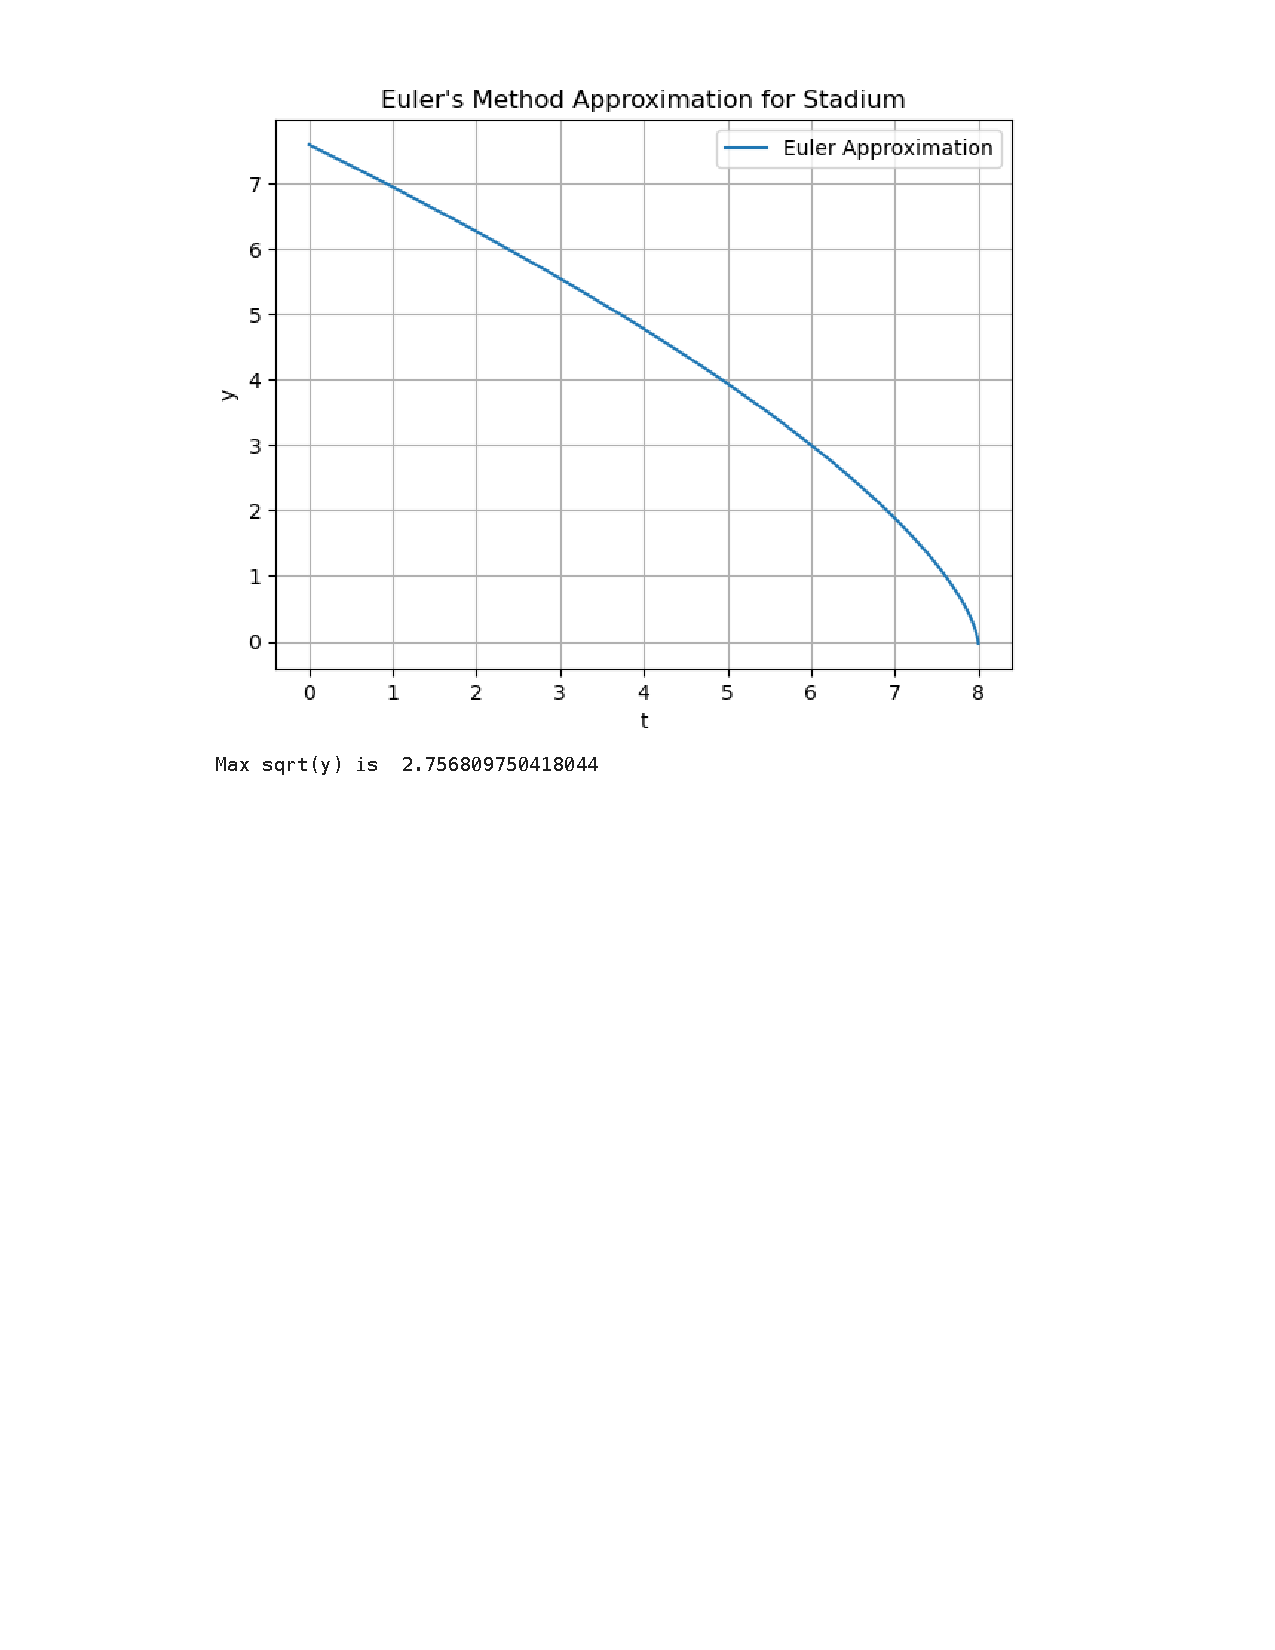
\includegraphics[width=0.4\textwidth]{python/Stadium-Euler-ipynb.pdf}


\end{slide}	
\end{solution}







\addcontentsline{toc}{subsection}{Numerical Methods for ODEs}

\addcontentsline{toc}{subsubsection}{Euler Method}
\addcontentsline{toc}{subsubsection}{Heun Method}


\begin{slide}

\question

Numerical Methods for:
\[ y' = f(t,y) \]

\SavedDefinitionRender{EulerMethod}

\SavedDefinitionRender{HeunMethod}

\end{slide}

\addcontentsline{toc}{subsubsection}{Runge-Kutta (4th order) Method}

\begin{slide}


\SavedDefinitionRender{RK4Method}


Desmos with all these three methods:
\hfil 
\url{https://www.desmos.com/calculator/haolaltd9s}


Consider the ODE $\dfrac{dy}{dx} = 2x\sin(x^2)$.
\begin{parts}
	\item Recall the meaning of the line segments in the slope field for this ODE.

	\item Consider the solution satisfying $y(0)=0$. With a step $h=0.1$, find the largest interval that the approximations stay within 0.1 distance of the exact solution.

\end{parts}

	
\end{slide}




\begin{solution}
\begin{slide}

The exact solution is 
\[
y = 1 - \cos(x^2).
\]

And by observing it on Desmos: 
\begin{center}
	\url{https://www.desmos.com/calculator/qflikqjufs}
\end{center}

We conclude that
\begin{itemize}
	\item Euler: $x< 1.2$
	\item Heun: $x < 5.6$
	\item Runge-Kutta: all $x$ ?
\end{itemize}
	
\end{slide}
	
\end{solution}



\addcontentsline{toc}{subsection}{Dimensional Analysis}

\begin{slide}

\question 

\textbf{Dimensional Analysis}

\SavedDefinitionRender{FundamentalDimensions}

\begin{parts}

\item When can we add/subtract quantities? With different dimensions? With the same dimensions?

\item When can we equate quantities? With different dimensions? With the same dimensions?

\item When can we multiply/divide quantities? With different dimensions? With the same dimensions?

\item It is convenient to define some functions as a power series (e.g. $e^x = 1 + x + \frac{x^2}{2} + \frac{x^3}{6}+ \cdots$). What condition on the dimension of $x$ is required to be able to do this?

\item What are the dimensions of a derivative $\frac{dy}{dx}$? What are the dimensions of an integral $\int y \, dx$?
	
\end{parts}

\begin{slidesonly}
	\bigskip
\end{slidesonly}


\textbf{Modelling:} Relationship between the variables in a model must be dimensionally consistent.

\end{slide}




\begin{slide}

\question \label{q:radioactive}

\paragraph{Non-Dimensionalization.}

Consider the model for a mass undergoing radioactive decay:
\[ \frac{dm}{dt} = -km \]
with $m(0) = m_0$.

\begin{parts}
	\item What are the units of $k$? What are the units of $t_c=\frac{1}{k}$? % $t_c$ is related to the half-life of the radioactive decay

	\item Introduce new variables: $\tau = \frac{t}{t_c}$ and $\overline{m}(\tau) = \frac{m(t)}{m_0}$. What is the ODE satisfied by $\overline{m}(\tau)$? What are its units? What are the parameters for this equation?
	
\end{parts}

\end{slide}




\begin{solution}
\begin{slide}

\begin{parts}
	\item The units of m are mass $M$, so the units of $\frac{dn}{dt}$ are $\frac{M}{T}$.
	
	This means that the units of $k$ must be $\frac{1}{T}$, so that $km$ matches the units on the other side of the equation.
	
	This implies that $t_c$ has the units of time $T$.
	
	\item $\displaystyle\frac{d\overline{m}}{d\tau} = \frac{1}{m_0} \frac{dm}{d\tau} = \frac{1}{m_0} \frac{dm}{dt} \frac{dt}{d\tau} = \frac{t_c}{m_0} \frac{dm}{dt}$
	
	So we get 
	\[
	\frac{d\overline{m}}{d\tau} 
		= \frac{t_c}{m_0} \frac{dm}{dt} 
		= -\frac{t_c}{m_0} k m(\tau)
		= -\frac{1}{m_0} m(\tau)
		= - \overline{m}
	\]
	and $\overline{m}(0)=1$.
	
\end{parts}
\end{slide}

\end{solution}

	







\begin{slide}
\question \label{q:budworms}
	
\begin{problem}[Spruce Budworm Outbreak]
Consider the model for spruce budworm outbreak in Eastern Canada\footnote{See ``Nonlinear Dynamics and Chaos'' by Strogatz.}.

\[
\frac{dN}{dt} = R N \left( 1 - \frac{N}{K} \right) - \frac{B N^2}{A^2 + N^2}.
\]

The first term accounts for resource-limited population growth within a tree and the second term accounts for the predation of the budworms by birds.
\end{problem}

\begin{parts}
	\item What are the units of $N, A, B, K$?
	


	\item To ``non-dimensionalize'' this ODE, what variable would you consider instead of $N$?  What ODE is satisfied by your new variable? How many parameters do you have now?
	
%	What is the ODE satisfied by $x(\tau)$?

	
\end{parts}

\end{slide}

\begin{solution}
\begin{slide}

\begin{parts}
	\item \begin{itemize}
		\item $[N] =$ budworm population ($N$)
		\item $[K] =$  carrying capacity of budworm population ($N$)
		\item $[R] =\frac{1}{T}$ 
		\item $[A] = N$
		\item $[B] = \frac{N}{T}$
 	\end{itemize}
 	
 	\item Consider the new variables\footnote{This is not the only way to do this.}:
		\begin{itemize}
			\item $x = N/A$ the non-dimensional budworm population
			\item $\tau = \frac{Bt}{A}$ the non-dimensional time
			\item $r = \frac{RA}{B}$ the non-dimensional growth rate
			\item $k = \frac{K}{A}$ the non-dimensional carrying capacity
		\end{itemize}


	\begin{align*}
		\frac{dx}{d\tau} 
			& = \frac{1}{A} \frac{dN}{dt} \frac{dt}{d\tau}
			= \frac{1}{B} R N \left( 1 - \frac{N}{K} \right) - \frac{N^2}{A^2 + N^2} \\
			& = \frac{1}{B} A R x \left( 1 - A\frac{x}{K} \right) - \frac{x^2}{(1 + x^2)} \\
			& = r x \left(1-\frac{x}{k}\right)- \frac{x^2}{(1 + x^2)}
	\end{align*}


	OR consider the new variables:
	\begin{itemize}
		\item $x = N/K$ non-dimensional budworm population (fraction of its carrying capacity)
		\item $b = B/K$ with units 1/(amount$^2 \times$ time
		\item $a = A/K$ non-dimensional
	\end{itemize}
	
	\begin{align*}
		\frac{dx}{d\tau} 
			& = \frac{1}{K} \frac{dN}{dt} \frac{dt}{d\tau}
			= R x \left( 1 - x \right) - \frac{1}{K}\frac{B N^2}{A^2 + N^2} \\
			& = R x \left( 1 - x \right) - \frac{b x^2}{a + x^2}
	\end{align*}


	
\end{parts}	
	
\end{slide}

\end{solution}	







\addcontentsline{toc}{subsubsection}{Buckingham Pi Theorem}

\begin{slide}

\question

\SavedDefinitionRender{DimensionalMatrix}

\SavedDefinitionRender{BuckinghamPiThm}
	
%	\begin{center}
%		\begin{tikzpicture}[scale=0.5]
%		  \draw[fill=brown!65!black,draw=none] (-1,0.1) rectangle (1,0);
%		  \draw (-1,0) -- (1,0);
%		  \draw[ultra thick] (0,0) -- (1,-4);
%		  \draw[thick, fill=black!20!white] (1,-4) circle (0.5) node {m};
%		%  \draw[dashed, gray] (0,0) -- (0,-4);
%		%  \draw[->,gray] (0,-3) node[above] {$\quad\theta$} arc (-90:-76:3);
%		%  \draw[->] (1, -4.75) -- (1, -5.25) node[below] {\small $\vec{F}_g$};
%		%  \draw[->] (1.1, -3.3) -- (0.95, -2.7) node[right] {\small $\vec{T}$};  
%		\end{tikzpicture}
%	\end{center}	


%\begin{minipage}{.15\textwidth}
%	\begin{center}
%		\begin{tikzpicture}[scale=0.6]
%		  \draw[fill=brown!65!black,draw=none] (-1,0.1) rectangle (1,0);
%		  \draw (-1,0) -- (1,0);
%		  \draw[ultra thick] (0,0) -- (1,-4);
%		  \draw[thick, fill=black!20!white] (1,-4) circle (0.5) node {m};
%		%  \draw[dashed, gray] (0,0) -- (0,-4);
%		%  \draw[->,gray] (0,-3) node[above] {$\quad\theta$} arc (-90:-76:3);
%		%  \draw[->] (1, -4.75) -- (1, -5.25) node[below] {\small $\vec{F}_g$};
%		%  \draw[->] (1.1, -3.3) -- (0.95, -2.7) node[right] {\small $\vec{T}$};  
%		\end{tikzpicture}
%	\end{center}	
%\end{minipage}
%	%
%\begin{minipage}{.35\textwidth}
%Consider a pendulum. We make assumptions:
%	\begin{itemize}
%		\item The pivot is frictionless
%		\item The rod is massless
%		\item Air resistance is neglected
%%		\item The gravitational field is uniform
%		\item The ceiling is infinitely rigid
%		\item $\cdots$
%	\end{itemize}
%\end{minipage}
%
%\bigskip
%\bigskip
%\bigskip

\begin{problem}
	Consider a pendulum. We make assumptions:

	\begin{minipage}{2.5in}
			\begin{itemize}
				\item The pivot is frictionless
				\item The rod is massless
				\item Air resistance is neglected
		%		\item The gravitational field is uniform
				\item The ceiling is infinitely rigid
				\item $\cdots$
			\end{itemize}		
	\end{minipage}
	\begin{minipage}{0.5in}
		\begin{tikzpicture}[scale=0.5]
		  \draw[fill=brown!65!black,draw=none] (-1,0.1) rectangle (1,0);
		  \draw (-1,0) -- (1,0);
		  \draw[ultra thick] (0,0) -- (1,-4);
		  \draw[thick, fill=black!20!white] (1,-4) circle (0.5) node {m};
		%  \draw[dashed, gray] (0,0) -- (0,-4);
		%  \draw[->,gray] (0,-3) node[above] {$\quad\theta$} arc (-90:-76:3);
		%  \draw[->] (1, -4.75) -- (1, -5.25) node[below] {\small $\vec{F}_g$};
		%  \draw[->] (1.1, -3.3) -- (0.95, -2.7) node[right] {\small $\vec{T}$};  
		\end{tikzpicture}
	\end{minipage}	
\end{problem}


\begin{parts}
	\item What are the units of the following variables of interest?
	\begin{enumerate}
		\item Period of the swing $[P] =$ 
		\item Pendulum mass $[m]=$
		\item Pendulum rod length $[\ell]=$
		\item Gravitational acceleration $[g]=$
		\item Amplitude of the swing $[\Theta]=$
	\end{enumerate}
	

\end{parts}

\end{slide}

\begin{slide}

\begin{parts}
\setcounter{partsitem}{1}

	\item Let us create the dimensional matrix:
	\begin{itemize}
		\item One column for each variable of interest (remember the order used for later)
		\item One row for each dimension
		\item Each term contains the power of the corresponding dimension for the corresponding variable
	\end{itemize}
	
	\begin{center}
	\begin{tabular}{cccccccl}
		& $[P]$ & $[m]$ & $[\ell]$ & $[g]$ & $[\Theta]$ & \\
		& $\downarrow$ & $\downarrow$ & $\downarrow$ & $\downarrow$ & $\downarrow$ & \\
	\multirow{3}{*}{$\mathcal{D}=\left[\begin{matrix} \, \\ \,\\ \, \end{matrix}\right.$} 
		& & & & & & 
		\multirow{3}{*}{$\left.\begin{matrix} \, \\ \,\\ \, \end{matrix}\right]$}
		& $\leftarrow M$
		\\
		& & & & & & & $\leftarrow L$ \\
		& & & & & & & $\leftarrow T$
	\end{tabular}
	\end{center}
	
	\item What is the rank of this matrix?
	\item What is the dimension of the null space? %\footnote{Use the Rank-nullity theorem.}?
	\item Find a basis for the null space.

\end{parts}

\end{slide}

\begin{slide}

For each vector of the null space basis, 
\[ \mat{2\\0\\-1\\1\\0} , \mat{0\\0\\0\\0\\1} \]

Buckingham Pi Theorem states that these correspond to non-dimensional variables $\Pi_1$ and $\Pi_2$:
\[ \Pi_1 = \frac{P^2 g}{\ell} \quad \text{ and } \quad \Pi_2 = \Theta \]

and that there is a relation between them:
\[
F(\Pi_1,\Pi_2)=0 \quad \text{ or } \quad \Pi_1 = f(\Pi_2) \quad \Leftrightarrow \quad \frac{P^2 g}{\ell} = f(\Theta)
\]
which implies that
\[ 
P = \sqrt{\frac{\ell}{g}} \cdot \overline{f}(\Theta),
\]
or in other words, the fact that the \textit{period of the pendulum is proportional to the square root of its length} is a consequence of a pure dimensional analysis of the variables in the problem.


\begin{parts}
	\setcounter{partsitem}{5}
	\item Recall the ODE for the pendulum: $ \frac{d^2\theta}{dt^2} = -\frac{g}{\ell}\sin (\theta)$. Linearize\footnote{If you are not comfortable with linearization of an ODE, check exercise 61 on \url{https://raw.githubusercontent.com/siefkenj/IBLODEs/main/dist/odes.pdf}.} it near the equilibrium $\theta=0$.
	\item Solve the linearized pendulum ODE, and compare the period of the linearized model to the nonlinear one.
\end{parts}


\end{slide}





\begin{slide}

\question

\begin{problem}

Consider the flow past a sphere.

\begin{center}
\begin{tikzpicture}
	\draw (0,0) circle (1);
	\draw[dashed] (0,0) ellipse (1cm and 0.25cm);
    \draw[variable=\t,domain=180:360,samples=100] plot ({cos(\t)},{0.25*sin(\t)});
    \foreach \i in {-0.9,-0.5,...,0.9}:
       \draw[-latex] (-2.5,{\i}) -- (-1.5,{\i});
\end{tikzpicture}
\end{center}

You don't need to know much about fluid dynamics to be able to deduce some properties of the flow. \\

The sphere is in a fluid (water) and we measure the force necessary to keep the sphere from moving downstream.

We want to understand how the drag force depends on the upstream velocity.
\end{problem}

\begin{parts}
	\item What are the units of the variables of interest\footnote{This choice is part of the modelling process.}?
	\begin{enumerate}
		\item drag force $[F]=$
		\item upstream velocity $[v]=$
		\item fluid density $[\rho]=$
		\item sphere diameter $[D]=$
		\item fluid viscosity\footnote{Fluid viscosity is the sphere's resistance to deformation by shear stress. To help with the units, the formula for the Force from viscosity is $F =\mu \cdot A \cdot u/y$, where $A$ is area, $u$ is velocity and $y$ is position.} $[\mu]= $
	\end{enumerate}
	\item Create a dimension matrix $\mathcal{D}$.
	\item What is its rank? What is the dimension of its null space? Find a basis for its null space.
	\item What are the non-dimensional variables $\Pi$'s from Buckingham Pi Theorem?
	\item What relations do you obtain?
		
\end{parts}
	
\end{slide}


\begin{solution}
\begin{slide}

Solution:

\[ \mathcal{D} = 
	\mat{1 & 0 & 1  & 0 & 1 \\
		1 & 1 & -3 & 1 & -1 \\
		-2 & -1 & 0 & 0 & -1}
\]
for rows $M,L,T$.

Its rank is 3, so there are 2 independent null vectors:
\[ \mat{0\\1\\1\\1\\-1} \quad \text{ and } \quad \mat{1\\-2\\-1\\-2\\0}
\]
corresponding to
\[
\Pi_1 = \frac{\rho v D}{\mu}
\quad \text{ and } \quad 
\Pi_2 = \frac{F}{\frac12\rho v^2 D^2}
\]

\begin{itemize}
	\item $\Pi_1 = $ Reynolds number (Re) which determines the relation between inertia and viscous forces in a fluid flow.
	\item $\Pi_2 = $ is the drag coefficient ($C_d$)
\end{itemize}

So dimensional analysis reveals:
\[ \Pi_2 = f(\Pi_1) \]
which means that the drag coefficient depends on the fluid's Reynolds number. \\

\hrule

Could have also obtained
\[ \mat{0\\1\\1\\1\\-1} \quad \text{ and } \quad \mat{1\\0\\1\\0\\-2} \]
which gives a different $\Pi_2$ and a different relation.
\end{slide}


\begin{slide}

	Using python to find the null space gives yet another set of different $\Pi_1$ and $\Pi_2$.

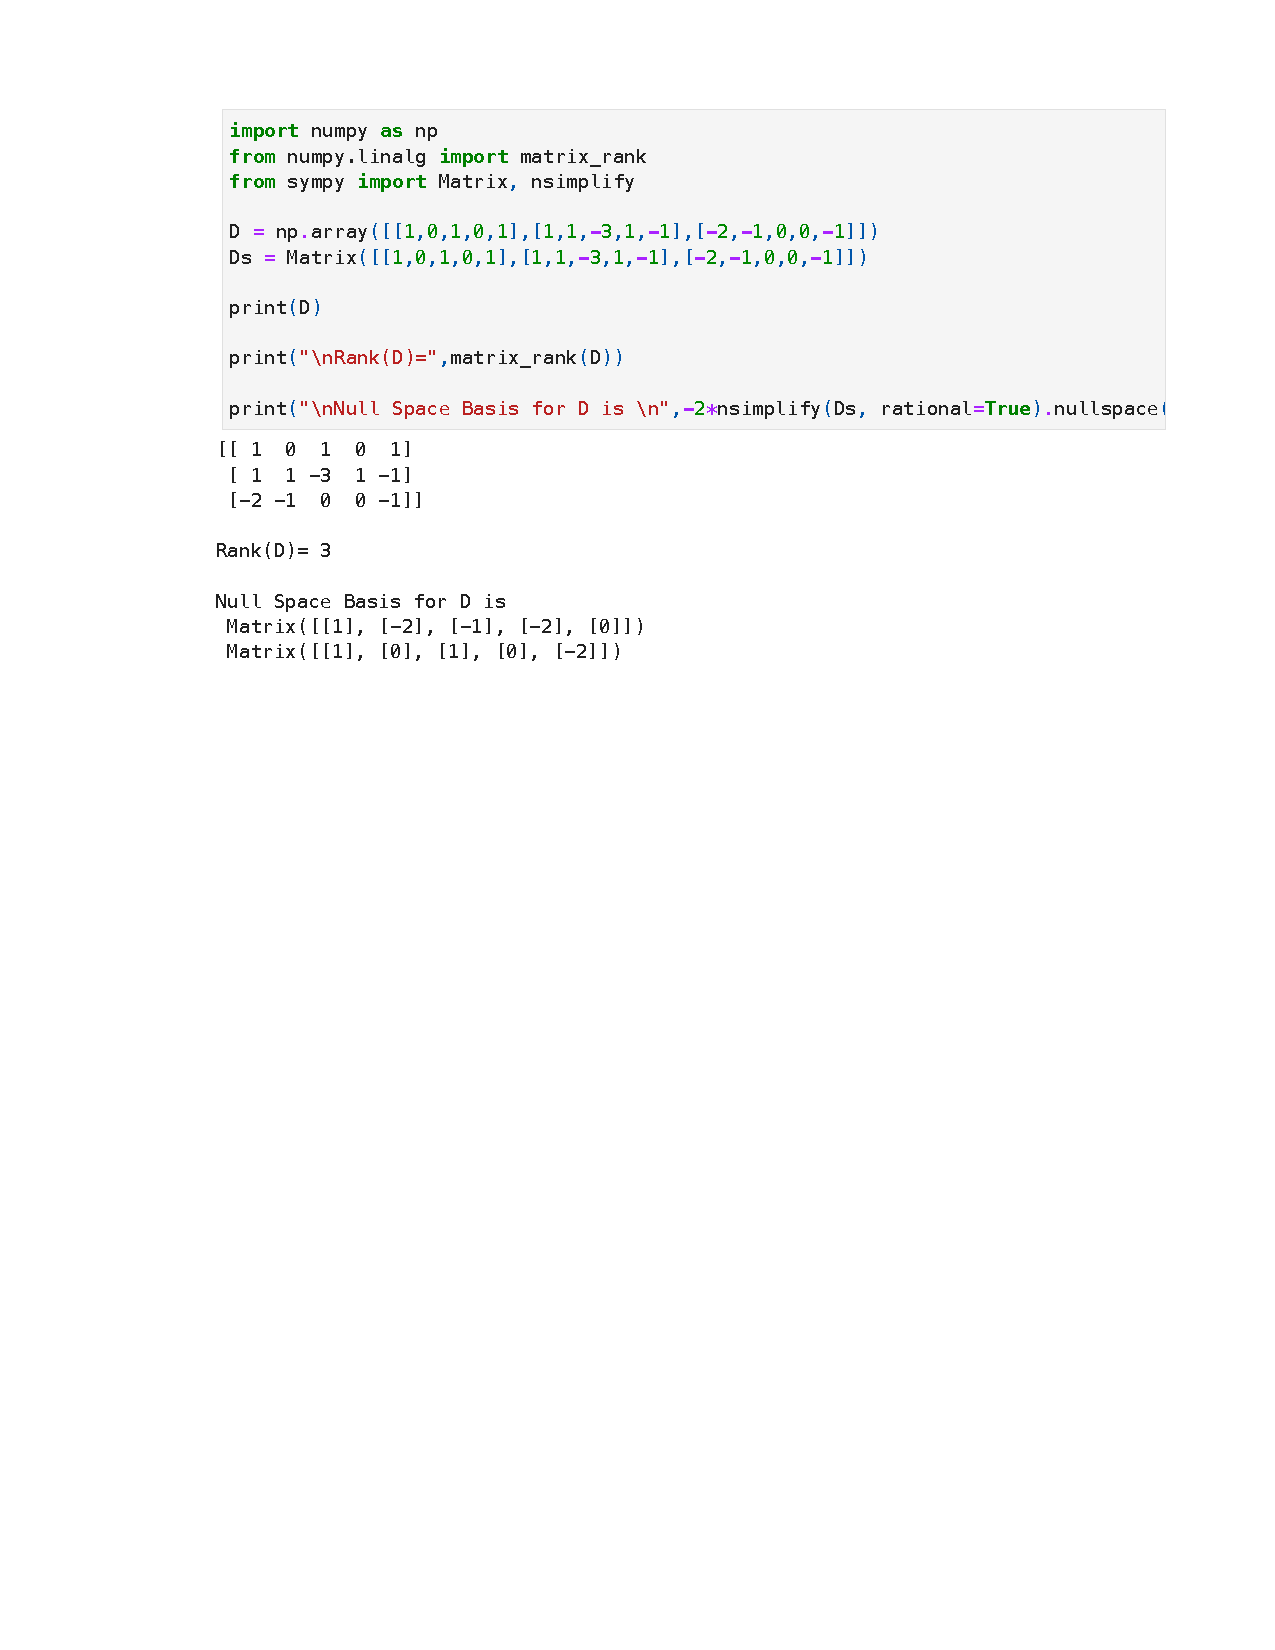
\includegraphics[width=0.75\textwidth]{python/sphere-dimensionanalysis.pdf}

	
\end{slide}
\end{solution}


\begin{slide}

\question

\begin{parts}
	\item Use Buckingham Pi Theorem on Exercise \ref{q:radioactive} about radioactive decay.
	\item Use Buckingham Pi Theorem on Exercise \ref{q:budworms} about the budworm population.
\end{parts}
	
\end{slide}





%
%\begin{slide}
%
%\question
%
%\begin{problem}[Dog Shampoo]
%Scientists are testing the effect of different dog shampoos. Let
%\begin{itemize}
%	\item $F = $ number of fleas (in millions)
%	\item $D = $ number of dogs (in thousands)
%	\item $a = $ effect of different dog shampoos
%\end{itemize}
%and consider the model: % for the interaction between them:
%\begin{align*}
%	F' & = -(1+a)F + D - 2 \\
%	D' & = -2F + (1-a)D + 1
%\end{align*}
%
%which is based on the following premises:
%\begin{itemize}
%	\item[(P1$_F$)] Ignoring all else, the number of parasites decays in proportion to its population (with constant $1+a$).
%	\item[(P2$_F$)] Ignoring all else, parasite numbers grow in proportion to the number of hosts (with constant 1).
%	\item[(P1$_D$)] Ignoring all else, hosts numbers grow in proportion to their current number (with constant $1-a$).
%	\item[(P2$_D$)] Ignoring all else, host numbers decrease in proportion to the number of parasites (with constant 2).
%	\item[(P1$_C$)] Anti-flea collars remove 2 million fleas per year.
%	\item[(P2$_C$)] Constant dog breeding adds 1 thousand dogs per year.
%\end{itemize}
%\end{problem}
%
%\begin{parts}
%	\item How are the premises expressed in the differential equations?
%	\item Find the equilibrium solutions for each value of $-1 \leq a \leq $.
%	\item Use \href{https://utoronto.syzygy.ca/jupyter/user-redirect/git-pull?repo=https://github.com/bigfatbernie/IBLMathModeling&subPath=book/python/fleas_dogs.ipynb}{\tt fleas_dogs.ipynb} and eigenvalues to check the stability\footnote{If you are not comfortable with studying the stability of the equilibrium solutions of a system of ODEs, then check exercises 32--61 of the same textbook. You can also check sections 2.4 and 2.5 of the textbook \href{https://raw.githubusercontent.com/siefkenj/IBLODEs/main/diffyqs-by-jiri-lebl/diffyqs.pdf}{\tt ``Diffy Qs'' by Jiri Lebl}.} of the equilibrium points for different values of $-1 \leq a \leq 1$.
%\end{parts}
%
%
%
%
%\end{slide}




\addcontentsline{toc}{subsection}{Modelling with Systems of ODEs}


\begin{slide}

\question

\begin{problem}[Dog Shampoo]\label{flea_dog}
Scientists are testing the effect of different dog shampoos. Let
\begin{itemize}
	\item $F = $ number of fleas (in millions)
	\item $D = $ number of dogs (in thousands)
	\item $a = $ effect of different dog shampoos
\end{itemize}
and consider the model: % for the interaction between them:
\begin{align*}
	F' & = -(1+a)F + D - 2 \\
	D' & = -2F + (1-a)D + 1
\end{align*}

which is based on the following premises:
\begin{itemize}
	\item[(P1$_F$)] Ignoring all else, the number of parasites decays in proportion to its population (with constant $1+a$).
	\item[(P2$_F$)] Ignoring all else, parasite numbers grow in proportion to the number of hosts (with constant 1).
\begin{slidesonly}
	\vspace{3cm}
\end{slidesonly}
	\item[(P1$_D$)] Ignoring all else, hosts numbers grow in proportion to their current number (with constant $1-a$).
	\item[(P2$_D$)] Ignoring all else, host numbers decrease in proportion to the number of parasites (with constant 2).
	\item[(P1$_C$)] Anti-flea collars remove 2 million fleas per year.
	\item[(P2$_C$)] Constant dog breeding adds 1 thousand dogs per year.
\end{itemize}
\end{problem}

\begin{parts}
	\item How are the premises expressed in the differential equations?
	\item Find the equilibrium solutions for each value of $-1 \leq a \leq 1$.
	\item Use \href{https://utoronto.syzygy.ca/jupyter/user-redirect/git-pull?repo=https://github.com/bigfatbernie/IBLMathModeling&subPath=book/python/fleas_dogs.ipynb}{\tt fleas_dogs.ipynb} and eigenvalues to check the stability\footnote{If you are not comfortable with studying the stability of the equilibrium solutions of a system of ODEs, then check exercises 32--61 of the \href{https://raw.githubusercontent.com/siefkenj/IBLODEs/main/dist/odes.pdf}{\texttt{MAT244 in-class exercises}}. You can also check sections 2.4 and 2.5 of the textbook \href{https://raw.githubusercontent.com/siefkenj/IBLODEs/main/diffyqs-by-jiri-lebl/diffyqs.pdf}{\texttt{``Diffy Qs'' by Jiri Lebl}.}} of the equilibrium points for different values of $-1 \leq a \leq 1$.
\end{parts}




\end{slide}






\addcontentsline{toc}{subsubsection}{Linearization of ODEs}


\begin{slide}

\question

\begin{problem}[Mammalian Circadian Clock]\label{circadian}

\begin{center}
 \begin{tikzpicture}[scale=0.65]
 
        % Setup the style for the states
        \tikzset{node style/.style={state, 
                                    minimum width=1.0cm,
                                    line width=0.5mm,
                                    fill=gray!20!white}}
        % Draw the states
        \node[draw,line width=0.5mm,fill=gray!20!white] at (0, 0)     (eb)     {E-Box};
        \node[node style] at (5, 2)     (mn)     {mRNA};
        \node[node style] at (5, 5.5)     (mc)     {mRNA};
        \node[node style] at (0, 5.5)     (pc)     {\textbf{PER}};
        \node[node style] at (0, 2)     (pn)     {PER};

        \draw[dashed] (-1,4.3) -- (6,4.3);
%        \draw[thick] (-1,-0.4) -- (0.8,-0.4) -- (0.8, 0.3) -- (1.8,0.3);
        % Connect the states with arrows
        \draw[every loop,
              auto=right,
              line width=0.5mm,
              >=latex,
              draw=black,
              fill=black]
            (eb) edge[bend left=10] node {transcription} (mn)
            (mn) edge[] node {nuclear export} (mc)
            (mc) edge[] node {translation} (pc)
            (pc) edge[] node {nuclear import} (pn)
            (pn) edge[] node {inhibition} (eb);
    \end{tikzpicture}
%    \caption{A diagram of the transcription-translation feedback loop of the mammalian circadian clock. When the enhancer-box (E-Box) on the DNA is active, messenger RNA (mRNA) is produced. The mRNA is exported from the nucleus where it is translated into PER protein. The protein is imported into the nucleus where it inhibits the the E-Box. \label{fig:circadianTTFL}}
\end{center}

When the enhancer-box (E-Box) on the DNA is active, messenger RNA (mRNA) is produced. The mRNA is exported from the nucleus where it is translated into PER protein. The protein is imported into the nucleus where it inhibits the E-Box. It is the cytosolic concentration of PER (highlighted) that indicates the time of day.

\begin{slidesonly}
	\vspace{2cm}
\end{slidesonly}

We get the model:
\begin{itemize}
	\item $x_1 = $ enhancer box on the DNA (E-box)
	\item $x_2, x_3 = $ mRNA inside/outside the nucleus
%	\item $x_3 = $ mRNA outside the nucleus
	\item $x_4, x_5 = $ PER outside/inside the nucleus
%	\item $x_5 = $ PER inside the nucleus
\end{itemize}
We get:

\hfil \begin{minipage}{.4\textwidth}
\begin{align*}
	x_1' & = -x_1 + e^{-\alpha x_5} \\
	x_2' & = -x_2 + x_1 \\
	x_3' & = -x_3+ x_2 
\end{align*}	
\end{minipage}
\quad 
\begin{minipage}{.4\textwidth}
\begin{align*}
	x_4' & = -x_4 + x_3 \\
	x_5' & = -x_5+ x_4 
\end{align*}	
\end{minipage}

where the exponential term represents the fact that the PER protein inhibits the E-box with ``strength'' $\alpha$.
\end{problem}

\begin{parts}
	\item Find an approximation for the equilibrium solution for $\alpha = 1$.
	\item This is a nonlinear problem. To linearize\footnote{If you are not comfortable with linearization of a system of ODEs, check exercise 61 on \url{https://raw.githubusercontent.com/siefkenj/IBLODEs/main/dist/odes.pdf}.} it around an equilibrium solution, find the Jacobian (or total derivative) $J$.
	\item Use \href{https://utoronto.syzygy.ca/jupyter/user-redirect/git-pull?repo=https://github.com/bigfatbernie/IBLMathModeling&subPath=book/python/circadian.ipynb}{\tt circadian.ipynb} and eigenvalues to check the stability of the equilibrium points for different values of $\alpha \in [0,100]$.
\end{parts}

%
%\paragraph{TO DO:} CREATE python that takes alpha and computes the jacobian matrix, its eigenvalues and graphs the real part of the eigenvalues as a function of alpha.



\end{slide}


\begin{solution}

\begin{slide}

\begin{parts}
	\item We get: $x_1 = x_2 = x_3 = x_4 = x_5$ and
	\[ x_5 = e^{-\alpha x_5} \]
	
	We have to approximate the solutions to this equation, e.g. using Newton's method.
	
	\item The Jacobian is:
		\[ J = 
			\mat { 	-1 & 0 & 0 & 0 & -\alpha e^{-\alpha x_5} \\
					1 & -1 & 0 & 0 & 0 \\
					0 & 1 & -1 & 0 &  0 \\
					0 & 0 & 1 & -1 &  0 \\
					0 & 0 & 0 & 1 & -1 
					}
		\]	
	\item The solutions are in \href{https://utoronto.syzygy.ca/jupyter/user-redirect/git-pull?repo=https://github.com/bigfatbernie/IBLMathModeling&subPath=book/python/circadian.ipynb}{\tt circadian5-sol.ipynb}.
	
	Basically we need to find the (5) eigenvalues for each value of $\alpha \in [0,100]$ and check when:
	\begin{itemize}
		\item All negative $\Rightarrow $ stable equilibrium
		\item One positive $\Rightarrow $ unstable equilibrium
	\end{itemize}
	
	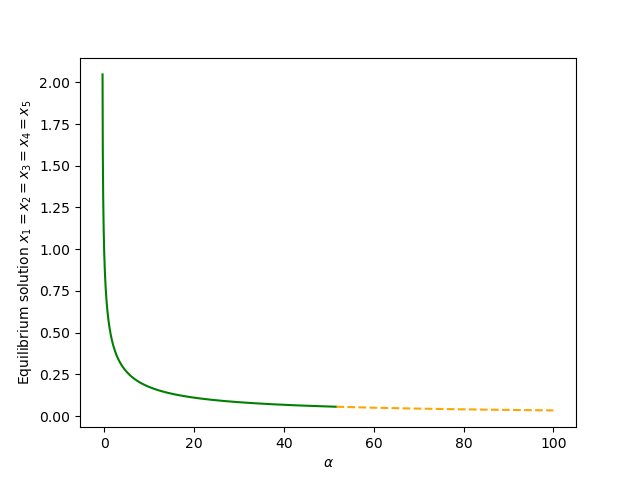
\includegraphics[width=200pt]{images/circadian5.png}
	
	
	Observe that in this case, we are actually looking for the \textbf{unstable} regime, when periodic solutions appear -- check the last part of the \texttt{Jupyter Notebook}. These only appear when the feedback in strong enough.
\end{parts}
	
\end{slide}	
\end{solution}



\addcontentsline{toc}{subsection}{ODE Bifurcations}


\begin{slide}
\question

From the previous question, we obtained equilibrium solutions that changed from stable to unstable as we changed the parameter $\alpha$ -- see the graph below.
	\begin{center}
		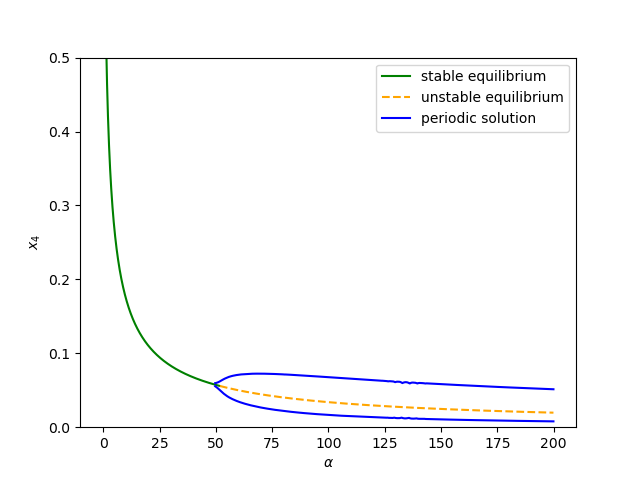
\includegraphics[width=225pt]{images/circadian5-periodic.png}
	\end{center}

This is called a \textbf{bifurcation}. \\

%\bigskip

Another type of bifurcation involves the creation of disappearance of equilibria as a parameter changes.

There are several typical types of bifurcations.

\end{slide}


\begin{slide}

\SavedDefinitionRender{bifurcations}

Decide on the type of bifurcation for each ODE.

\begin{parts}
	\item The ODE from Exercise \ref{flea_dog}.
	\item The system of ODEs from Exercise \ref{circadian}.
	\item The ODE $\frac{dx}{dt} = rx - x^2$.
	\item The ODE $\frac{dx}{dt} = r + x^2$.
	\item The ODE $\frac{dx}{dt} = rx - x^3$.
	\item The following system of ODEs as $\mu$ changes: \\
	$ \begin{cases}
 		\frac{dx}{dt} & = \mu x -  \omega y \\[5pt]
 		\frac{dy}{dt} & = \omega x + \mu y
	\end{cases}
	$
	\item The Lotka-Volterra model for $0< a < 1$: \\
	$ \begin{cases}
 		\frac{dx}{dt} & = a xy - x - 2 + \frac1a\\[5pt]
 		\frac{dy}{dt} & = y - \frac12 xy - 2 + \frac1a
	\end{cases}
	$
\end{parts}
	
	
\end{slide}


\begin{solution}
\begin{slide}
\begin{parts}
	\item Change of stability bifurcation
	\item Hopf bifurcation
	\item Transcritical bifurcation: $x(r-x) = 0$ so $x=0$ and $x=r$ are equilibria and they swap stability at $r=0$.
	\item Saddle-node bifurcation: equilibria only exist for $r<0$, one stable and one unstable.
	\item Pitchfork bifurcation: $x(r-x^2)=0$ implies
	\begin{itemize}
		\item $r\leq 0$: equilibria at $x=0$
		\item $r>0$: equilibria at $x=0$ and $x=\pm \sqrt{r}$
	\end{itemize}
	See \url{https://www.desmos.com/calculator/uksexnwbdz} about pitchfork perturbation.
	\item Hopf bifurcation: Equilibrium at $(0,0)$ and with eigenvalues $\mu \pm \omega i$, so
	\begin{itemize}
		\item $\mu<0$: stable spiral
		\item $\mu = 0$: stable centre (periodic orbit)
		\item $\mu > 0$: unstable spiral
	\end{itemize}
	\item Equilibrium at $(\frac{1}{a},2)$ and
	\begin{itemize}
		\item $a < 1-\frac{\sqrt{3}}{2} \approx 0.134$: two negative eigenvalues (stable)
		\item $1-\frac{\sqrt{3}}{2}< a < \frac12$: stable spiral
		\item $ a = \frac12$: stable centre (periodic orbit)
		\item $ a > \frac12$: unstable spiral
	\end{itemize}
	
	Change in qualitative behaviour at $a = 1-\frac{\sqrt{3}}{2}$ and Hopf at $a = \frac12$.
	
	Calculations at \href{https://utoronto.syzygy.ca/jupyter/user-redirect/git-pull?repo=https://github.com/bigfatbernie/IBLMathModeling&subPath=book/python/bifurcation-LotkaVolterra.ipynb}{\tt bifurcation-LotkaVolterra.ipynb}.
	
	Visualize also here \url{https://www.desmos.com/calculator/aydzcpccy4}

\end{parts}
	
\end{slide}
	
\end{solution}








\addcontentsline{toc}{subsection}{Modelling with PDEs}

\begin{slide}
\question \label{transport}

\begin{problem}[Transport Equation]
	
Consider a river with the water moving at speed $v$.
\begin{center}
\includegraphics*[width=175pt]{images/river.pdf}
\end{center}

We want to model $w(x,t)$, the density of pollutant in the river at the point $x$ and time $t$.
\end{problem}

\begin{parts}
\item How much pollutant is there in $[a,b]$?
\item How does pollutant change in $[a,b]$?
\item Find a ``conservation of pollutant'' equation.
\item Simplify the equation to obtain a PDE for $w(x,t)$.

\textit{Hint: Recall the FTC: $f(b)-f(a) = \int_a^b f'(x) dx$.}

\end{parts}


\end{slide}


\begin{solution}
\begin{slide}

\begin{parts}
	\item $\displaystyle T(t) = R \int_a^b w(x,t) ~dx$	, 	where $R$ is the width of the river.
	\item Pollutant goes in through the left and out through the right, so the change in the amount of pollutant is
	\[
	w(a,t) v R - w(b,t) v R = v R \bigskip(w(a,t) - w(b,t)\big).
	\]

	\item Because pollutant is neither created or destroyed, we know that:
	\[T'(t) = v R \bigskip(w(a,t) - w(b,t)\big) \]
	
	\begin{slidesonly}
	\vspace{3cm}
	\end{slidesonly}	
	
	\item \hfil \\[-35pt]
	\begin{align*}
		R \int_a^b \frac{\partial w}{ \partial t} (x,t) \, dx & = v R \bigskip(w(a,t) - w(b,t)\big) \\
		\int_a^b \frac{\partial w}{ \partial t} (x,t) ~dx & = v \bigskip(w(a,t) - w(b,t)\big) \\
		\int_a^b \frac{\partial w}{ \partial t} (x,t) ~dx & = -v \int_a^b \frac{\partial w}{\partial x} (x,t) ~dx
	\end{align*}
	\[
	\int_a^b \frac{\partial w}{ \partial t} + v \frac{\partial w}{ \partial x} ~dx = 0
	\]
	
	Because $a,b$ are arbitrary points in the river, we can conclude that
	\[ 
	\frac{\partial w}{ \partial t} + v \frac{\partial w}{ \partial x} = 0
	\qquad \text{ or } \qquad 
	w_t + v \cdot w_x = 0
	\]
	
\end{parts}

	Here is a Jupyter notebook with the Lax-Friedrichs Method approximation for the transport equation:
	\begin{itemize}
		\item \href{https://utoronto.syzygy.ca/jupyter/user-redirect/git-pull?repo=https://github.com/bigfatbernie/IBLMathModeling&subPath=book/python/transport_LaxFriedrichs.ipynb}{\tt transport\_LaxFriedrichs.ipynb}
	\end{itemize}
	
\end{slide}
	
\end{solution}


\addcontentsline{toc}{subsubsection}{Method of Characteristics}


\begin{slide}
\question

\SavedDefinitionRender{characteristics}
	
\begin{parts}

	\item Find the solution of the transport equation from Exercise \ref{transport} using the Method of Characteristics with the initial condition $u(x,0) = p(x)$.
	
	\item Find the solution of the same problem with an accelerating river: $v = 3t^2$.
	
	\item Find the solution for $w_t + 5 w_x = 2$.

	\item Find the solution for $w_t + 3t^2 w_x = 2$.

	\item Find the solution for $w_t + 3t^2 w_x = -x$.
	
\end{parts}

\begin{center}
	\begin{tikzpicture}[scale=1.5]
		\draw[gray] (-0.4,0)--(0,0);
		\draw[latex-latex, gray] (3,0) node[above] {$x$} -- (0,0) -- (0,2) node[right] {$t$};
		\draw[orange, thick] (0.5,0) node[below] {$x_0$} -- (2.5,1.5) node[above] {$x=vt+x_0$};
		\foreach \i in {0,0.4,0.8,1.2}:
			\draw[dashed, blue,variable=\x,domain=-0.75:2.75,samples=50] plot ({\x+4*\i/3},{sin(\x*180)*(-1.2*\x*\x*\x*\x+3.7*\x*\x*\x-5.8*\x)/20+0.04+\i});
		\draw[blue] (-0.75,0) node {$u(x,0)$};
	\end{tikzpicture}
	\end{center}	
	
	

\end{slide}
%
%
%\begin{slide}
%
%\begin{center}
%	\begin{tikzpicture}[scale=1.5]
%		\draw[gray] (-0.4,0)--(0,0);
%		\draw[latex-latex, gray] (3,0) node[above] {$x$} -- (0,0) -- (0,2) node[right] {$t$};
%		\draw[orange, thick] (0.5,0) node[below] {$x_0$} -- (2.5,1.5) node[above] {$x=vt+x_0$};
%		\foreach \i in {0,0.4,0.8,1.2}:
%			\draw[dashed, blue,variable=\x,domain=-0.75:2.75,samples=50] plot ({\x+4*\i/3},{sin(\x*180)*(-1.2*\x*\x*\x*\x+3.7*\x*\x*\x-5.8*\x)/20+0.04+\i});
%		\draw[blue] (-0.75,0) node {$u(x,0)$};
%	\end{tikzpicture}
%	\end{center}	
%\end{slide}


\begin{solution}

\begin{slide}
\begin{parts}

	\item We need to solve
	
	\begin{itemize}
		\item $	\frac{dx}{dt} = v \quad \to$  an observer moving along the river at the same speed as the river
		\item $ \frac{du}{dt} = 0 \quad \to $ for such an observer looking at the river, the pollutant density doesn't change
	\end{itemize}

		\[
	\begin{cases}
		x = vt + x_0 \\
		u\big(x(t),t\big) = C
	\end{cases}
	\]
	
	This means that when $t=0$, we get $u(x_0,0) = C = p(x_0)$, and $x_0 = x - vt$, so
	\[
	u(x,t) = C = p(x_0) = p(x-vt).
	\]
	
	The idea in a graph:
	\begin{center}
	\begin{tikzpicture}
		\draw (-1,0)--(0,0);
		\draw[latex-latex] (3,0) node[above] {$x$} -- (0,0) -- (0,2) node[right] {$t$};
		\draw[red, thick] (0.5,0) node[below] {$x_0$} -- (2.5,1.5) node[above] {$x=vt+x_0$};
%		\draw[red, thick] (0.5,0) node[below] {$x_0$} -- node[above, rotate=37] {$x=vt+x_0$}(2.5,1.5);
		\foreach \i in {0,0.4,0.8,1.2}:
			\draw[dashed, gray,variable=\x,domain=-0.75:2.75,samples=50] plot ({\x+4*\i/3},{sin(\x*180)*(-1.2*\x*\x*\x*\x+3.7*\x*\x*\x-5.8*\x)/20+0.04+\i});
		\draw[gray] (-1,0) node {$u(x,0)$};
	\end{tikzpicture}
	\end{center}

	Here we can run an approximation for a specific $u(x,0)$ and $v = -1.2$: 
	\begin{itemize}
		\item \href{https://utoronto.syzygy.ca/jupyter/user-redirect/git-pull?repo=https://github.com/bigfatbernie/IBLMathModeling&subPath=book/python/transport_LaxFriedrichs.ipynb}{\tt transport\_LaxFriedrichs.ipynb}
	\end{itemize}

	\item The idea is similar but we get 
	
			\[
	\begin{cases}
		x = t^3 + x_0 \\
		u\big(x(t),t\big) = C
	\end{cases}
	\]
	
	This means that when $t=0$, we get $u(x_0,0) = C = p(x_0)$, and $x_0 = x - t^3$, so
	\[
	u(x,t) = C = p(x_0) = p(x-t^3).
	\]

		
\end{parts}

\end{slide}
	
\end{solution}




\addcontentsline{toc}{subsubsection}{Traffic Flow Model}


\begin{slide}

\question

\begin{problem}[Traffic Flow]
\begin{center}
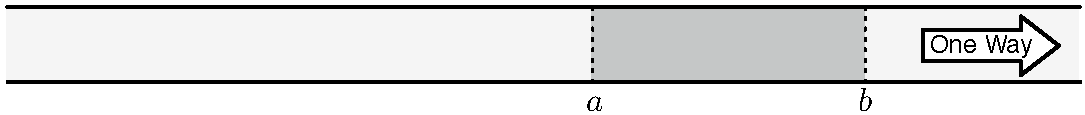
\includegraphics[width=0.9\textwidth]{images/road-long.pdf}
\end{center}
We want to model how traffic flows on a one way road.
\end{problem}

Let
\begin{itemize}
\item $\rho(x,t) = $ density of cars (number of cars per $km$) %at position $x$ and time $t$;
\item $\phi(x,t) = $ number of cars passing the point $x$ per hour % at time $t$ 
			% $=$ flux of cars.
\end{itemize}

And assume:
\begin{itemize}
	\item[(C)] Cars are conserved (they are not destroyed nor created on the road)
\end{itemize}

\begin{parts}
\item What is the total number of cars in the section of the road $x \in [a,b]$ at time $t$?

\item How does the total number of cars change in $[a,b]$?


\item Obtain an equation relating $\rho(x,t)$ and $\phi(x,t)$. The equation should not include $a$ or $b$.	

\end{parts}


\end{slide}



\begin{slide}


We need to model how fast cars move on the road: $\phi(x,t)$.

Below we graphed measurements for density and speed at the highway 401\footnote{Data from the paper \href{https://doi.org/10.1287/trsc.1090.0297}{``Calibrating Steady-State Traffic Stream and Car-Following Models Using Loop Detector Data'' by H Rakha and M Arafeh}} together with three different models to fit the data.
\begin{center}
\begin{tikzpicture}[scale=0.8]
    \begin{axis}[
            width=10cm, height=5cm, %, width=15cm, height=8cm,     % size of the image
            grid = major,
            grid style={dashed, gray!30},
            xmin=0,xmax=60,ymin=0,ymax=120,
%			minor y tick num=5,
			ytick distance = 20,
            ylabel=speed $v$ (km/h),
            xlabel=density $\rho$ (vehicles/km),
            clip mode=individual % so that the fits go on top of the data
         ]
        \addplot[only marks] table  {images/densityspeed.dat};
        \addplot[domain=0:60, very thick, samples=121, color=blue]{121.2613*(1-x/63.6628)}; % Greenshields
        \addplot[domain=0:60, very thick, samples=121, color=orange]{106.6081*(1-exp(-56.1848*(1/x-1/56.5544)))}; % Newell
        \addplot[domain=0:60, very thick, samples=121, color={black!60!green}]{109.7737/(1+exp(0.1297*(x-32.2037)))}; % logistic
    \end{axis}
\end{tikzpicture}
\end{center}

It shows three models:
\begin{itemize}
	\item[\textcolor{blue}{\textbullet}] \textcolor{blue}{Greenshields model} (linear fit of the data): $v(\rho) = v_{\max} \left(1 - \dfrac{\rho}{\rho_{\max}}\right)$
	\item[\textcolor{orange}{\textbullet}] \textcolor{orange}{Newel model}
	\item[\textcolor{black!60!green}{\textbullet}] \textcolor{black!60!green}{Logistic model}: $v(\rho) = v_{\max} / \left(1+ e^{-k(\rho - \rho_0)}\right)$
\end{itemize}

\begin{parts}
\setcounter{partsitem}{3}
	\item Using the Greenshields model, find an expression for $\phi(x,t)$.	
	\item Obtain a PDE for $\rho(x,t)$.
\end{parts}

	
\end{slide}


\begin{solution}
\begin{slide}

\begin{parts}
	
	\item $\displaystyle C(t) = \int_a^b \rho(x,t) ~dx$
	\item $\displaystyle C'(t) = \phi(a,t) - \phi(b,t)$
	\item From the previous two parts, we get
	\[ 
		\int_a^b \rho_t ~dx = \phi(a,t) - \phi(b,t)
	\]

	By using the FTC, we have $\displaystyle \phi(b,t) - \phi(a,t) = \int_a^b \phi_x(x,t) ~dx$, so we conclude that
	\[ 
		\int_a^b \rho_t + \phi_x(x,t) ~dx = 0
	\]
	Because this integral must be true for any values of $a,b$, we conclude that the integrand must be zero:
	\[ 
		\rho_t + \phi_x(x,t) = 0
	\]	
	
	
	\item $\phi(x,t) = \rho v(\rho)$
	\item We can expand the equation we found before:
	\begin{align*}
		\rho_t + \phi_x(x,t) & = 0 \\
		\rho_t + \rho_x v_{\max} \left(1 - \dfrac{\rho}{\rho_{\max}}\right) - \rho v_{\max} \dfrac{\rho_x}{\rho_{\max}} & = 0 \\
		\rho_t + \rho_x v_{\max} \left(1 - \dfrac{2 \rho}{\rho_{\max}}\right) & = 0
	\end{align*}

\end{parts}
	
\end{slide}
	
\end{solution}





\begin{slide}
\question

Let us study two interesting cases.

\begin{parts}
\item[]
\begin{center}
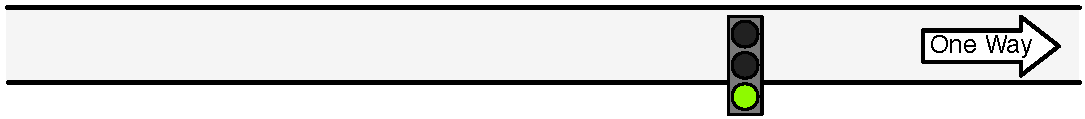
\includegraphics[width=.6\textwidth]{images/road-green.pdf}	
\end{center}


\item What is the initial car density $\rho(x,0) = \rho_0(x)$ on a one way road with a traffic light that just turned from \textbf{\textcolor{red}{red}} to \textbf{\textcolor{green}{green}}?


\begin{center}
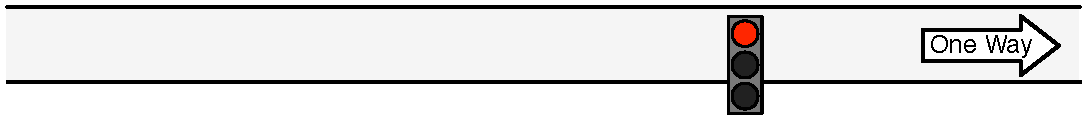
\includegraphics[width=.6\textwidth]{images/road-red.pdf}	
\end{center}


\item To model a light turning from \textbf{\textcolor{green}{green}} to \textbf{\textcolor{red}{red}}, we need to be more creative. What is an initial car density $\rho(x,0) = \rho_0(x)$ that will guarantee incoming cars have to stop at the red light?

	
\end{parts}
	
\end{slide}





\begin{slide}
\question \label{traffic:red}

\begin{problem}[Traffic flow scenario]

We want to solve the following traffic flow problem:
\begin{align*}	
	& \rho_t + v_{\max} \left( 1 - \frac{2 \rho}{\rho_{\max}}\right) \rho_x = 0  \tag{Traffic flow model} \\
	& r(x,0) = f(x) = 
		\begin{cases}
			\rho_{\min}	& \text{ for } x<0\\
			\rho_{\max}	& \text{ for } x>0
		\end{cases}
\end{align*}

Consider the following parameters: 
\begin{itemize}
	\item $v_{\max}=60$
	\item $\rho_{\max} = 120$
	\item $\rho_{\min} = 20$
\end{itemize}
\end{problem}


\begin{parts}
	\item What are the moving observers (characteristics) $x(t)$ for this problem?
	\item What is the density $\rho(x,t)$?
	\item Sketch the characteristics and mark the values of $\rho$ on the same graph below.
	
	\begin{center}
	\begin{tikzpicture}
		\draw[-latex] (0,-0.5) -- (0,2) node[left] {$t$};
		\draw[-latex] (-2.5,0) -- (2.5,0) node[above] {$x$};	
	\end{tikzpicture}
	\end{center}

	
	\item What is $\rho(0,2)$?
\end{parts}

	
\end{slide}



\addcontentsline{toc}{subsubsection}{Shockwaves and Rankine-Hugoniot condition}


\begin{slide}
\question
When characteristics intersect, this means that the solution \textbf{cannot be continuous}.

So we need to find a \textbf{discontinuous} solution.

\begin{itemize}
\item Assume that the discontinuity forms a curve $x_s(t)$.
\end{itemize}

\begin{center}
	\begin{tikzpicture}
		\draw[-latex] (0,-0.5) -- (0,2.5) node[left] {$t$};
		\draw[-latex] (-2.5,0) -- (2.5,0) node[above] {$x$};	
		\draw[thick,blue] (-2,0) node[below] {$\rho_1$} -- (2.5,2.5);
		\draw[thick,green!50!black] (0.5,0) node[below] {$\rho_2$} -- (1,2.5);
		\draw[thick, fill=white] (0.8125,1.5625) circle (0.1);
	\end{tikzpicture}	
	\qquad 
	\begin{tikzpicture}
		\draw[-latex] (0,-0.5) -- (0,2.5) node[left] {$t$};
		\draw[-latex] (-2.5,0) -- (2.5,0) node[above] {$x$};	
		\draw[thick, blue] (-2,0) node[below] {$\rho_1$} -- (0.8125,1.5625);
		\draw[thick, green!50!black] (0.5,0) node[below] {$\rho_2$} -- (0.8125,1.5625);
		\draw[orange, ultra thick, variable=\x,domain=0:0.72,samples=20] plot({\x+0.8125},{1.5625+0.4*\x-9*\x*\x*\x+\x+12*\x*\x*\x*\x}) node[right] {$x_s(t)$};
		\draw[thick, fill=white] (0.8125,1.5625) circle (0.1);
	\end{tikzpicture}	
\end{center}



\begin{parts}
	\item What should the discontinuity $x_s(t)$ be?
\end{parts}
	
\end{slide}


\begin{slide}
\question

We need to step back for a moment and review some Calculus.

Consider a function
\[
F(x) = \int_0^z g(x) ~dx
\]
and consider a differentiable function $h(t)$.

\begin{parts}
	\item What is $F'(z)$?
	\item What is $F'\big(g(t)\big)$? 
	 	\qquad What is $\left[ F\big(h(t)\big) \right]'$?

	\item What is $\displaystyle \left[ \int_0^{h(t)} g(x) ~dx \right]'$?
		\qquad  What is $\displaystyle \left[ \int_{h(t)}^1 g(x) ~dx \right]'$?

\end{parts}

\end{slide}



\begin{slide}
\question
We need to go back to the derivation of the traffic flow model.

We had the following:
\[
\frac{d}{dt} \left[ \int_a^b \rho(x,t) ~dx \right] = \phi(a,t) - \phi(b,t)
\]

We then took the derivative inside the integral, because we assumed that the density $\rho$ was differentiable (thus continuous). Now we know it is not, so we must break up the interval of integration into ``chunks'' where $\rho$ is continuous.

We now assume that $\rho(x,t)$ is discontinuous across $x=x_s(t)$.

\begin{parts}
	\item Expand the left-hand side of the equation into integrals with continuous integrands.
	\item We know that $\phi = \phi(\rho)$. Take the limits
	\[ a \to \big(x_s(t)\big)^- \quad \text{ and } \quad b \to \big(x_s(t)\big)^+ \]
	and obtain an ODE for $x_s(t)$.
	
	This ODE is called the \textbf{Rankine-Hugoniot shockwave condition}.
	
\end{parts}
	
\end{slide}


\begin{solution}

\begin{slide}

\begin{parts}

\item We have
\begin{multline*}	
	\frac{d}{dt} \left[ \int_a^b \rho(x,t) ~dx \right] \\
		= \frac{d}{dt} \left[ \int_a^{x_s(t)} \rho(x,t) ~dx + \int_{x_s(t)}^b \rho(x,t) ~dx \right]
\end{multline*}

Using the previous exercise, we get
%\[\rho\big(x_s^-(t),t\big) x_s'(t) - \rho\big(x_s^+(t),t\big) x_s'(t)	+ \int_a^b \rho_t(x,t) ~dx \]
\[
\left[\rho\big(x_s^-(t),t\big)- \rho\big(x_s^-(t),t\big) \right] x_s'(t) + \int_a^b \rho_t(x,t) ~dx
\]

	\item Let us define the following
	\begin{itemize}
		\item $\displaystyle\rho^-(t) = \lim_{x \to x_s^-(t)} \rho(x,t)$
		\item $\displaystyle\rho^+(t) = \lim_{x \to x_s^+(t)} \rho(x,t)$
	\end{itemize}
	
%	Then we have
%	\[
%	\left[\rho\big(x_s^-(t),t\big)- \rho\big(x_s^-(t),t\big) \right] x_s'(t) + \int_a^b \rho_t(x,t) ~dx
%		= \phi\big(\rho(a,t)\big)	 - \phi\big(\rho(b,t)\big)
%	\]
	So when we take the limits, we obtain
	\[
		( \rho^-(t) - \rho^+(t)) x_s'(t) = \phi(\rho^-(t)) - \phi(\rho^+(t)) 
	\]
	We get
	\[
		x_s'(t) = \frac{\phi(\rho^-) - \phi(\rho^+)}{\rho^- - \rho^+}
	\]

	This condition is called the \textbf{Rankine-Hugoniot shockwave condition}.
\end{parts}

\end{slide}
\end{solution}




\begin{slide}
\question

\begin{parts}
	\item Use the Rankine-Hugoniot shockwave condition to find the full solution of Exercise \ref{traffic:red}.
	
	
	\item Compare the solution to the numerical solution using the Lax-Friedrichs method in \href{https://utoronto.syzygy.ca/jupyter/user-redirect/git-pull?repo=https://github.com/bigfatbernie/IBLMathModeling&subPath=book/python/traffic_flow_LaxFriedrichs.ipynb}{\tt traffic\_flow\_LaxFriedrichs.ipynb}.
	
	Note that to use this method, we wrote the PDE as
	$ \rho_t + \big( \phi(\rho) \big)_x = 0 $
	with $\phi(\rho) = v_{\max} \left( 1 - \frac{\rho}{\rho_{\max}}\right) \rho$.
	
	\textit{Note also that the method is very sensitive to the choice of $\Delta x$ and $\Delta t$: it only works when $\frac{\Delta t}{\Delta x}$ is small enough.}
		
	\begin{minipage}{.55\textwidth}
		\item Trace the paths of the cars starting at $x_0 = -10, -5, 0, 2.5$.
	\end{minipage}\hfil 
	\begin{minipage}{.4\textwidth}
	\begin{tikzpicture}[scale=0.85]
		\draw[-latex] (0,-0.1) -- (0,2) node[left] {$t$};
		\draw[-latex] (-2.5,0) -- (2.5,0) node[above] {$x$};	
	\end{tikzpicture}
	\end{minipage}
	
	
	\item What happens when cars slow down gradually? Find the solution for the initial condition
	\[	r(x,0) = f(x) = 
		\begin{cases}
			\rho_{\min}	& \text{ for } x<-1\\
			\rho_{\max} + (\rho_{\min}-\rho_{\max})x & \text{ for } -1 \leq x \leq 0 \\ 
			\rho_{\max} 	& \text{ for } x>0
		\end{cases}
	\]
	
	
	\item How would the model change if there is an on-ramp at $x=0$? 
	
\end{parts}

	
\end{slide}


\begin{solution}
\begin{slide}

\begin{parts}

\item The Rankine-Hugoniot condition yields:
\[
x'_s(t) = \frac{\phi(20) - \phi(120)}{20-120} = -\frac{1000 - 0}{100} = -10
\]
where we recall that $\displaystyle\phi(\rho) = v_{\max} \left( 1 - \frac{\rho}{\rho_{\max}}\right) \rho = 60 \left(1 - \frac{\rho}{120}\right) \rho$.

We also know that the discontinuity starts at the point $(x,t) = (0,0)$, so 
\[
x_s(t) = -10t
\]

\begin{minipage}{.5\textwidth}
This means that the solution is
\[
\rho(x,t) = 
	\begin{cases}
		\rho_{\min} & \text{ for } x < x_s(t) \\
		\rho_{\max} & \text{ for } x > x_s(t)
	\end{cases}
\]

In practice this means that cars are accumulating behind the traffic sign ($\rho_{\max}$) means cars are stopped.
The cars are accumulating at the speed of $10$ km/h.
\end{minipage}
\hfill
\begin{minipage}{.4\textwidth}
	\begin{tikzpicture}
		\draw[-latex] (0,-0.5) -- (0,2.5) node[left] {$t$};
		\draw[-latex] (-2.5,0) -- (2,0) node[above] {$x$};	
		\draw[thick, blue] (0,0) -- ({-2.5/5},2.5) node[above left] {$x=-10t$};
		\draw[green!50!black] (-1.5,1) node {$\rho(x,t) = \rho_{\min}$};
		\draw[red] (1,1.5) node {$\rho(x,t) = \rho_{\max}$};
%		\draw[thick,blue] (-2,0) node[below] {$\rho_1$} -- (2.5,2.5);
%		\draw[thick,green!50!black] (0.5,0) node[below] {$\rho_2$} -- (1,2.5);
%		\draw[thick, fill=white] (0.8125,1.5625) circle (0.1);
	\end{tikzpicture}	
\end{minipage}

\end{parts}
	
\end{slide}	
\end{solution}


\begin{solution}
\begin{slide}
\begin{parts}
\setcounter{partsitem}{1}
\item When we run the numerical solution \href{https://raw.githubusercontent.com/bigfatbernie/IBLMathModeling/main/book/images/traffic_flow-60.mp4}{(click here to see an animation)}, we get the following:

\hfil \begin{tabular}{c}
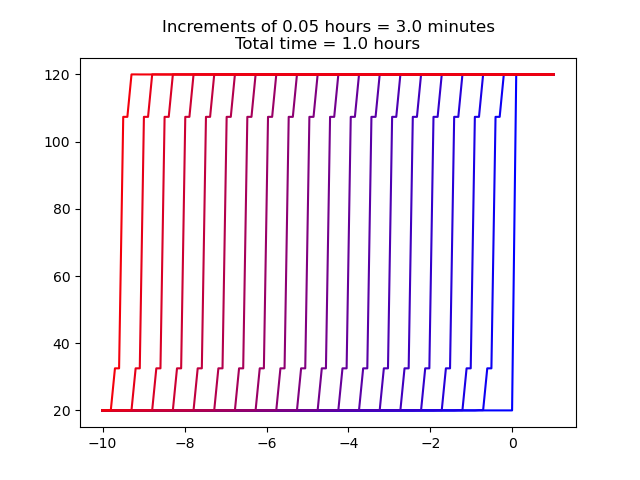
\includegraphics[width=.35\textwidth]{images/traffic_flow-60-deltax110.png} \\[-8pt]
larger $\Delta x$ and $\frac{\Delta t}{\Delta x} = 0.02$
\end{tabular}
\hfil \begin{tabular}{c}
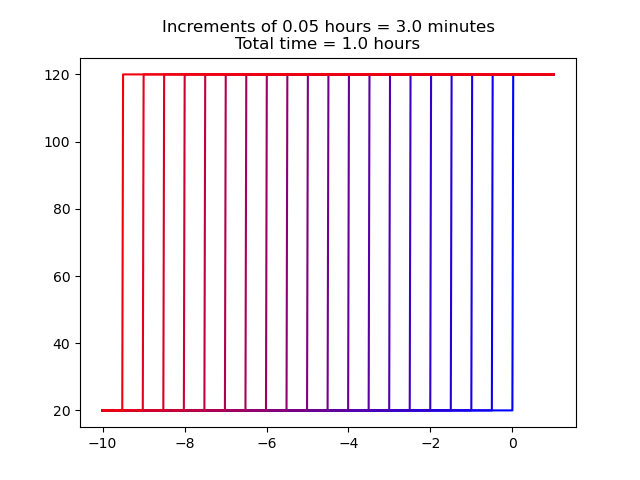
\includegraphics[width=.35\textwidth]{images/traffic_flow-60-deltax550.png} \\[-8pt]
smaller $\Delta x$ and $\frac{\Delta t}{\Delta x} = 0.1$
\end{tabular}

If the resolution in $x$ is not good enough, then we see some artifacts from the numerical approximation.

We can estimate the speed of the shockwave: it takes 4 time-steps to get to from $x=0$ to $x=-2$:
\begin{itemize}
	\item Speed of the shockwave $= \frac{2}{4 \cdot (0.05)} = 10$ km/h.
\end{itemize}

\end{parts}
\end{slide}

\begin{slide}

\begin{parts}
\setcounter{partsitem}{2}
\item 	 \hfill 

\def\tmax{0.3}
\begin{center}
	\begin{tikzpicture}[xscale=0.40,yscale=12]
		\draw[-latex] (0,{-\tmax/10}) -- (0,\tmax) node[right] {$t$};
		\draw[-latex] (-10,0) -- (5,0) node[above] {$x$};	
    	\draw[blue,dashed] (0,0) -- ({-\tmax*10},\tmax);
        \draw[yellow!90!black, thick] (2.5,0) node[below] {$2.5$} -- (2.5,\tmax);
        \draw[orange!50!yellow, thick] (0,0)  node[below] {$0$} -- (0,\tmax);
		\draw[orange, thick] (-5,0) node[below] {$-5$} -- ({-5+5*60/70},{5/70}) -- ({-5+5*60/70},\tmax);
    \draw[pink, thick] (-10,0) node[below] {$-10$} -- ({-10+10*60/70},{10/70}) -- ({-10+10*60/70},\tmax);
        \draw (-6.5,{\tmax/2}) node {$v = 60$ km/h};
        \draw (3,{\tmax/2}) node {$v = 0$ km/h};
	\end{tikzpicture}
\end{center}

Here is an animation of the solution: \href{https://raw.githubusercontent.com/bigfatbernie/IBLMathModeling/main/book/images/traffic_flow-animation.mp4}{traffic_flow-animation.mp4}



\item In this case, the shockwave doesn't start at $t=0$, but when the characteristics meet for the first time.

\end{parts}
	
\end{slide}
	
\end{solution}















%%%%%%%%%%%%%%%%%%%%%%%%%%%%%%%%%%%%%%%%%%%%%%%%%%%%%
%
%
%  	PROBABILITY MODELS - ODEs, Systems of ODEs, Bifurcation, PDEs, 
%
%
%%%%%%%%%%%%%%%%%%%%%%%%%%%%%%%%%%%%%%%%%%%%%%%%%%%%%

\phantomsection
\addcontentsline{toc}{section}{Probability Models}\label{sec:probability}


%%%%%%%%%%%%%%%%%%%%%%%%%%%%%%%%%%%%%%%%%%%%%%%%%%%%%
%
%
%  	PROBABILITY MODELS - 
%
%
%%%%%%%%%%%%%%%%%%%%%%%%%%%%%%%%%%%%%%%%%%%%%%%%%%%%%

\begin{slide}
\question

\begin{slidesonly}
	\vspace{3cm}
\end{slidesonly}

\begin{center}
\Huge 
\textcolor{LimeGreen}{Probability Models}
\end{center}

	
\end{slide}



\begin{slide}
\question

\SavedDefinitionRender{IntroProbability}

\SavedDefinitionRender{ConditionalProb}

\end{slide}

\begin{slide}

\SavedDefinitionRender{hazard}

\begin{parts}
	\item Show that $\frac{d\tilde{F}_T}{dt} = - f_T$. 
	\item Find an ODE that relates $\tilde{F}_T$ and $h(t)$ and use it to show that
	\[ \tilde{F}_T(t) = e^{-\int_{-\infty}^t h_T(\tau) ~d\tau} \]

	\item Show that the mean satisfies 
	\[\displaystyle 
		\mu_T = \int_{-\infty}^\infty \tilde{F}_T(t) ~dt.
	\]
\end{parts}
	
\end{slide}


\begin{slide}
\question \label{exponential}

\SavedDefinitionRender{Exponential}

Let us study the \textbf{exponential random variable}: 
\[T \sim {\rm Exp}(\gamma).\]

\begin{parts}
	\item Find an expression for its cdf $F_T(t)$.
	\item Find an expression for its ccdf $\tilde{F}_T(t)$.
	\item Find an expression for its hazard function $h_T(t)$.
	\item What is its mean $\mu_T$?
\end{parts}

\begin{slidesonly}
\vspace{3cm}	
\end{slidesonly}

The hazard function is a constant, so knowing that the random variable is yet to occur, doesn't us give any information.

\SavedDefinitionRender{memoryless}


\begin{parts}
\setcounter{partsitem}{4}
	\item Show that the Exponential is memoryless.
\end{parts}
	
\end{slide}


\begin{solution}
\begin{slide}
\begin{parts}

	\item $\displaystyle F_T(t) 
	 		= \int_{-\infty}^t f_T(\tau)~d\tau
	 		= \int_0^t \gamma e^{-\gamma \tau} ~d\tau
%	 		= - e^{-\gamma \tau} \big|_0^t 
	 		= 1-e^{-\gamma t}$
	 
	 \item $\tilde{F}_T(t) = 1 - F_T(t) = e^{-\gamma t}$.

	 \item $\displaystyle h_T(t) = \frac{f_T(t)}{\tilde{F}_T(t)} = \gamma$.

	 \item $\displaystyle \mu_T 
	 		= \int_{0}^\infty \tau f_T(\tau) ~d\tau
	 		= \int_0^\infty \tilde{F}_T(\tau) ~d\tau 
	 		= -\frac{1}{\gamma} e^{-\gamma \tau} \big|_0^\infty
	 		= \frac{1}{\gamma}$
	 	
	 \item 
	 $\displaystyle \Pr(T>t+s|T>t) = \frac{\Pr(T>t+s)}{\Pr(T>t)} = \frac{e^{-\gamma (t+s)}}{e^{-\gamma t}} = e^{-\gamma s} = \Pr(T>s)$.
	 
	

	
\end{parts}


	
\end{slide}

\end{solution}
	




\begin{slide}
\question

Backblaze is a cloud storage company that uses thousands of hard drives\footnote{They publish data on their hard drives \url{https://www.backblaze.com/b2/hard-drive-test-data.html}.}.\\

The failure rate for a hard drive, also known as hazard rate, is composed of three terms:
\begin{center}
\begin{tikzpicture}
	\draw[latex-latex] (6,0) --node[below] {time} (0,0) --node[above,rotate=90] {failure rate} (0,3.5);
	\draw[dashed,blue] (0,1) -- (5,1) node[below] {\scriptsize constant failures};
   \draw[dashed,orange!80!black,variable=\x,samples=100,domain=0:5] plot({\x},{2*exp(-\x)}) node[above] {\scriptsize early failures}; 
   \draw[dashed,green!80!black,variable=\x,samples=100,domain=0:5] plot({\x},{0.2+\x*\x/10}) node[above,rotate=45] {\scriptsize wear-out failures}; 
   \draw[thick,variable=\x,samples=100,domain=0:5] plot({\x},{1+\x*\x/10+2*exp(-\x)}); 
\end{tikzpicture}
\end{center}

When we add the three terms, we get a \textit{bathtub} curve. \\

Should Backblaze always use the hard drives with the longest mean time between failures (MTBF)?

\begin{parts}
\item Suppose that there are $N$ hard drive types, each with a known fixed cost $c_n$, a known profit $p_n$ per unit time that hard drive is operational, and a random lifetime $T_n$ with a known distribution. Backblaze has limited storage, so they can only have $M$ hard drives. If they use $x_n$ drives of type $n$, what is their profit function?

%$$
%P = \sum_{n=1}^N \left[p_n \sum_{m=1}^{x_n} T_n(m)  - x_n c_n \right]
%$$

\item What is their expected profit?
%$$
%\sum_{n=1}^N \left[x_n p_n \mu_{T_n}  - x_n c_n \right]
%$$

\item If they choose to maximize the expected profit, what is the solution?
\end{parts}

	
\end{slide}


\begin{slide}

This means that they will \textit{put all their eggs in one basket}!

This is a risky strategy. Especially if hard drives with long-lives have a large variance in those lives.

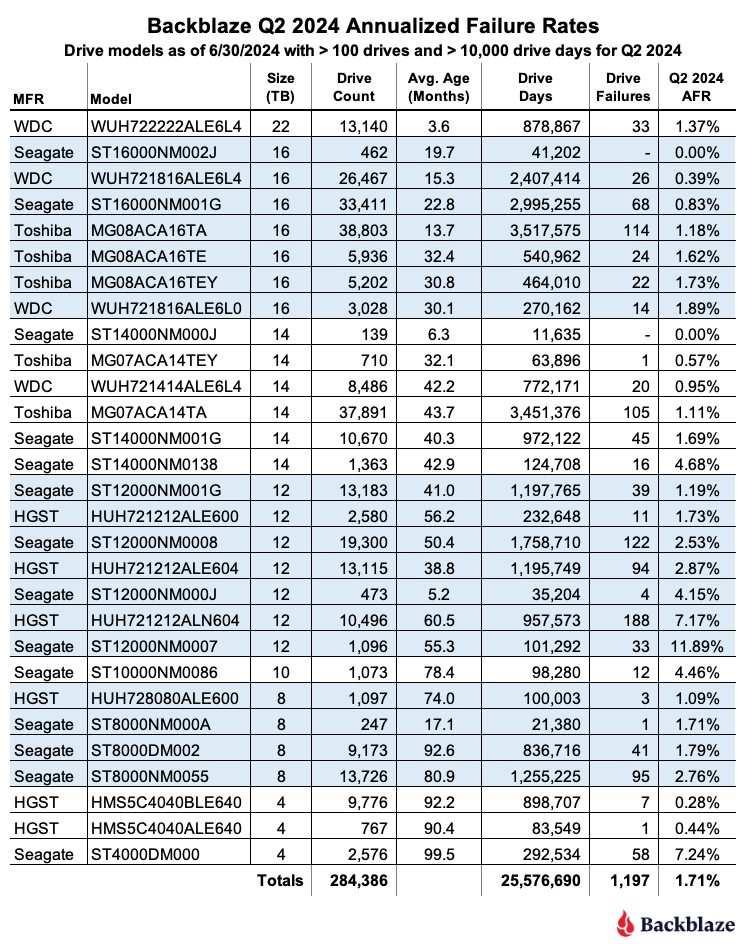
\includegraphics[width=150pt]{images/backblaze-hdd.png}

To account for this, we can add a constraint that the variance of the profit $\sigma_P^2$ not be too large.
This will result in a more diverse selection of hard drives.
Unfortunately, for most hard drive lifetime distributions, this constraint is non-linear in the decision variables. 

	
\end{slide}






\begin{slide}
\question \label{ex-poisson}

\SavedDefinitionRender{Poisson}

Start with $N(0) = 0$ and define $p_n(t) = \Pr\big( N(t)=n \big)$, the probability that $n$ events have occurred up to time $t$.


\begin{slidesonly}
	\bigskip
\end{slidesonly}

\begin{parts}
	\item What is $p_n(0)$?
	\item Take $n=0$. Explain in words why $p_0(t) = \tilde{F}_T(t)$.

	\item A different approach:
	\[ 
		\underbrace{\frac{d p_0}{dt}(t)}_{\substack{\text{change in prob}\\\text{that $N(t)=0$}}}
		 = +\underbrace{0}_{\text{can never increase}}
		 -\underbrace{p_{0}(t) h_T(t)}_{\substack{\text{decreases if $N$ was $0$}\\\text{and an event occurs}}}
	\]

	Solve this differential equation to find $p_0(t)$.

	\item For $n>0$, we can find an ODE in a similar way. The change in probability that $N(t)=n$:
	\begin{enumerate}
		\item decreases if ...
		\item increases if ...
	\end{enumerate}
	
	\item Obtain an ODE and show that $p_n(t) = \frac{(\gamma t)^n}{n!} e^{-\gamma t}$ is a solution.
	
	\item Show that it is normalized, i.e. $\displaystyle\sum_{n=0}^\infty p_n(t) = 1$.

	\item Calculate its mean $\displaystyle\sum_{n=0}^\infty n p_n(t)$.
	
	
\end{parts}

	
\end{slide}


\begin{solution}
	

\begin{slide}
\begin{parts}
	\item $p_n(0) = \delta_{n,0}$
	\item It is the probability that no events have occurred until time $t$, which is the complement of the probability of an event happening between time $0$ and $t$, so $p_0(t) = 1 - F_T(t) = \tilde{F}_T(t) = e^{-\gamma t}$.

	\item The ODE is $\frac{d p_0}{dt} = -\gamma p_0$, so the solution is $p_0(t) = e^{-\gamma t}$.

	\item 
	\begin{enumerate}
		\item increases if $N$ was $n-1$ and an event occurs imminently
		\item decreases if $N$ was $n$ and an event occurs imminently
	\end{enumerate}
	
	\item 	
	\[ 
		\underbrace{\frac{d p_n}{dt}(t)}_{\substack{\text{change in prob}\\\text{that $N(t)=n$}}}
		 = +\underbrace{p_{n-1}(t) h_T(t)}_{\substack{\text{increases if $N$ was $n-1$}\\\text{and an event occurs}}}
		 -\underbrace{p_{n}(t) h_T(t)}_{\substack{\text{decreases if $N$ was $n$}\\\text{and an event occurs}}}
	\]
	This gives 
	\[ 
		\frac{dp_n}{dt}(t) = \gamma p_{n-1}(t) - \gamma p_n(t)
	\]
	
	\item The series 
	\[ \sum_{n} \frac{(\gamma t)^n}{n!}  \]
	is the Taylor series for $e^{\gamma t}$.
	
	\item Consider $g_n(t) = \frac{(\gamma t)^n}{n!}$. Then
%	\[
%	g_n'(t) = n \frac{(\gamma t)^{n-1}}{n!}
%	\]
%	and
	\[t g_n'(t) = n g_n(t)\]
	So
	\[ \sum_n n \frac{(\gamma t)^n}{n!} 
		= t \left( \sum_n \frac{(\gamma t)^n}{n!}\right)'
		= t \left( e^{\gamma t} \right)'
		= t \gamma e^{\gamma t} \]
	Thus the mean is $E(N(t)) = \gamma t$, which is typically denoted by $\lambda$.

\end{parts}
	
\end{slide}
\end{solution}


\begin{slide}

\SavedDefinitionRender{Poisson2}
	
\end{slide}



\begin{slide}
\question \label{aquarium}
\begin{problem}[Aquarium Problem\footnote{based on a problem from Meerschaert's `Mathematical Modeling'.}]

A pet store sells large aquariums. They sell approximately \textbf{one aquarium per week} (call this the parameter $\lambda$).

Not wanting to maintain too much stock (the aquariums are large and fragile), the store orders 3 aquariums at the end of the week if they are completely out of stock.

How missed sales result from this policy?
\end{problem}

Let
\begin{itemize}
	\item $X_n = $ number of aquariums in stock at the beginning of week $n$
	\item $D_n=$ number of aquariums demanded in week $n$
\end{itemize}
Any available aquariums that are demanded are purchased and assume that when the store orders aquariums, they arrive right away.


\begin{parts}
	\item Why is $X_n$ random?
	\item Assume that $D_n$ is Poisson distributed. Why is this reasonable?
	\item Then what is $\Pr (D_n = k)$?
	\item There are only 3 states of $D_n$: 1, 2, 3. 
	
	The following diagram shows the possible changes in stock from one week to the next.
	
	Complete the following diagram with the probability of transitioning from one state to another for all the arrows except the ones marked with $\star$.
	
	\begin{center}
	\begin{tikzpicture}[font=\sffamily,scale=0.4]
	 
        % Setup the style for the states
        \tikzset{node style/.style={state, 
                                    minimum width=1cm,
                                    line width=0.3mm,
                                    fill=gray!20!white}}
 
        % Draw the states
        \node[node style] at (0, 0)     (x1)    {$X_n=1$};
        \node[node style] at (6, 0)     (x2)    {$X_n=2$};
        \node[node style] at (3, -5.196) (x3) 	{$X_n=3$};
 
        % Connect the states with arrows
        \draw[every loop,
              auto=right,
              line width=0.3mm,
              >=latex,
              draw=black,
              fill=black]
            (x1) edge[loop above]             node {} (x1)
            (x2) edge[loop above]             node {} (x2)
            (x3) edge[loop below]             node {$\star$} (x3)            
            (x1)     edge[bend right=20]            node {} (x2)
            (x2)     edge[bend right=20]            node {} (x1)
            (x1)     edge[bend right=20]            node {$\star$} (x3)
            (x3)     edge[bend left=20]            node {} (x2)
            (x2)     edge[bend left=20, auto=left] node {$\star$} (x3)
            (x3) edge[bend right=20, auto=right] node {} (x1);
    \end{tikzpicture}
	\end{center} 

	\item For the remaining arrows, marked with $\star$, observe that if there is one aquarium in inventory and 3 clients come, then the store will only be able to sell one of them and order new aquariums, so at the beginning of next week there will be 3 aquariums. Because of this, complete the  remaining $\star$ arrows by using the complementary probability. 

\end{parts}


\end{slide}


\begin{slide}

\begin{parts}
\setcounter{partsitem}{5}
	\item Create a transition matrix $\mathcal{P}$ with
	\begin{itemize}
		\item $P_{ij} = $ probability of transitioning from state $i$ to $j$
	\end{itemize}
	
	\item Let 
	\[ 
	\vec{\pi}_n = \mat{ 	\Pr(X_n = 1) \\
					\Pr(X_n = 2) \\
					\Pr(X_n = 3) }
	\]
	Find a relation between $\vec{\pi}_{n+1}$ and $\vec{\pi}_n$.
	
	\item Use \href{https://utoronto.syzygy.ca/jupyter/user-redirect/git-pull?repo=https://github.com/bigfatbernie/IBLMathModeling&subPath=book/python/aquarium.ipynb}{\tt aquarium.ipynb} to approximate the solution for the long term states. 
		Interpret the results.

	\item The original question was about how much business is the store missing. Write the expected percentage of weeks when the store lost at least one sale as a probability.
	
	\item Calculate $W$:
	\begin{align*}
	W 	& = \lim_{n \to \infty} \Pr(D_n > X_n) \\
		& = \lim_{n \to \infty} \sum_{i=1}^3 \Pr(D_n>X_n | X_n = i) \Pr (X_n = i),
	\end{align*}
	using the limiting vector $\vec{\pi}$ found. Interpret the result.
	
	\item We can calculate the average lost sales too by considering:
	\[
	L	= \lim_{n \to \infty} \sum_{i=1}^3 (D_n - i) \Pr(D_n>X_n | X_n = i) \Pr (X_n = i).
	\]
	
	Calculate $L$, the expected number of lost aquarium sales. Interpret the results.
	
	\item What is $S(L^\star, \lambda)$?
\end{parts}

	
\end{slide}




\begin{solution}
\begin{slide}
\begin{parts}
	\item Because $D_n$ is random.  
	\item Because the arrival of customers can happen at any time, they are independent of each other, and they don't depend on $t$ (in reality they do), but because we are measuring in weeks, it's ok.
	\item $\Pr(D_n=k) = \frac{\lambda^k}{k!} e^{-\lambda}$.
	\item 
	
	\begin{center}
	\begin{tikzpicture}[font=\sffamily,scale=0.5]
	 
        % Setup the style for the states
        \tikzset{node style/.style={state, 
                                    minimum width=1cm,
                                    line width=0.3mm,
                                    draw=black,
                                    fill=gray!20!white}}
 
        % Draw the states
        \node[node style] at (0, 0)     (x1)    {\textcolor{black}{$X_n=1$}};
        \node[node style] at (6, 0)     (x2)    {\textcolor{black}{$X_n=2$}};
        \node[node style] at (3, -5.196) (x3) 	{\textcolor{black}{$X_n=3$}};
 
        % Connect the states with arrows
        \draw[every loop,
              auto=right,
              line width=0.3mm,
              >=latex,
              draw=black,
              fill=black]
            (x1) edge[loop above]             node {$e^{-\lambda}$} (x1)
            (x2) edge[loop above]             node {$e^{-\lambda}$} (x2)
            (x3) edge[loop below]             node {$1-\lambda e^{-\lambda}-\frac{\lambda^2}{2}e^{-\lambda}$} (x3)            
            (x2)     edge[bend right=20]            node {$\lambda e^{-\lambda}$} (x1)
            (x1)     edge[bend right=20]            node {$1-e^{-\lambda}$} (x3)
            (x3)     edge[bend left=20]            node {$\lambda e^{-\lambda}$} (x2)
            (x2)     edge[bend left=20, auto=left] node {$1-e^{-\lambda}-\lambda e^{-\lambda}$} (x3)
            (x3) edge[bend right=20, auto=right] node {$\frac{\lambda^2}{2}e^{-\lambda}$} (x1);
    \end{tikzpicture}
	\end{center} 
	
%\setcounter{partsitem}{5}	
%
%	\item \[ 
%			\mathcal{P} 
%				= \mat{ 	e^{-\lambda} & 0 & 1 - e^{-\lambda} \\
%						\lambda e^{-\lambda} & e^{-\lambda} & 1 - e^{-\lambda} - \lambda e^{-\lambda} \\
%						\frac{\lambda^2}{2} e^{-\lambda} & \lambda e^{-\lambda} & 1 - \lambda e^{-\lambda} - \frac{\lambda^2}{2}e^{-\lambda} }
%			\]
%
\end{parts}
	
\end{slide}

\begin{slide}
\begin{parts}
\setcounter{partsitem}{5}	

	\item \[ 
			\mathcal{P} 
				= \mat{ 	e^{-\lambda} & 0 & 1 - e^{-\lambda} \\
						\lambda e^{-\lambda} & e^{-\lambda} & 1 - e^{-\lambda} - \lambda e^{-\lambda} \\
						\frac{\lambda^2}{2} e^{-\lambda} & \lambda e^{-\lambda} & 1 - \lambda e^{-\lambda} - \frac{\lambda^2}{2}e^{-\lambda} }
			\]

	\item We have $\vec{\pi}_{n+1} = \vec{\pi}_n \mathcal{P} 
		 				\quad \Leftrightarrow \quad \vec{\pi}_{n+1} = \mathcal{P}^T \vec{\pi}_n$.
	\item The long term result is: $\vec{\pi} = \mat{0.28471134 \\0.26313999 \\0.45214867}$.


	This means that with $\lambda =1$, that is with 1 expected customer per week, the store should expect to have :
	\begin{itemize}
		\item 1 aquarium in inventory 28.5\% of the weeks
		\item 2 aquariums in inventory 26.3\% of the weeks
		\item 3 aquariums in inventory 45.2\% of the weeks
	\end{itemize}
	
	This means that about half of the time, they have a full inventory. Perhaps this is due to the fact that they ran out of aquariums and just ordered more, so they might be losing a lot of sales when they run out of stock.
	
	\item It is the probability that the demand is higher than the inventory: $\Pr(D_n > X_n)$. 
	
	\begin{slidesonly}
		\bigskip	
	\end{slidesonly}

	\item $W$ is the long term expected percentage of weeks when sales are lost:\\[-20pt]
	\begin{align*}
		W 	
			& = \lim_{n \to \infty} \sum_{i=1}^3 \Pr(D_n>X_n | X_n = i) \Pr (X_n = i) \\
			& = \lim_{n \to \infty} \sum_{i=1}^3 \Pr (X_n = i) \sum_{j=i+1}^\infty \Pr(D_n=j)\\
			& = \sum_{i=1}^3 \pi_i \sum_{j=i+1}^\infty \frac{\lambda^j}{j!} e^{-\lambda} \\
			& = e^{-\lambda} \left[ \pi_1 \sum_{j=2}^\infty \frac{\lambda^j}{j!} + \pi_2  \sum_{j=3}^\infty \frac{\lambda^j}{j!} + \pi_3  \sum_{j=4}^\infty \frac{\lambda^j}{j!} \right]
	\end{align*}
	The series in $j$ is the tail of the Taylor series for the exponential $e^{\lambda}$, so we can write it as \\[-15pt]
	\begin{align*}
	W = & e^{-\lambda}  \left[ \pi_1 ( e^\lambda - 1 - \lambda ) + \pi_2 ( e^\lambda - 1 - \lambda - {\textstyle \frac{\lambda^2}{2}}) \right.\\ 
		& \left.+ \pi_3 ( e^\lambda - 1 - \lambda - {\textstyle \frac{\lambda^2}{2}- \frac{\lambda^3}{6}}) \right]
	\end{align*}
%	\begin{align*}
%	W = &   \left[ \pi_1 ( 1 - (1 + \lambda)e^{-\lambda} ) + \pi_2 ( 1 - (1 + \lambda + {\textstyle \frac{\lambda^2}{2}})e^{-\lambda}) \right.\\ 
%		& \left.+ \pi_3 (1 - (1 + \lambda + {\textstyle \frac{\lambda^2}{2} + \frac{\lambda^3}{6}})e^{-\lambda}) \right]
%	\end{align*}


	Using \href{https://utoronto.syzygy.ca/jupyter/user-redirect/git-pull?repo=https://github.com/bigfatbernie/IBLMathModeling&subPath=book/python/aquarium-sol.ipynb}{\tt aquarium-sol.ipynb}, we get $W = 0.105$, which means that the store loses sales about 11\% of the weeks.
	
\end{parts}


\end{slide}


\begin{slide}
\begin{parts}
\setcounter{partsitem}{10}
	\item Similarly, we can calculate $L =  0.14256$, so the store should expect to lose an average of 0.14 sales per week. 
	Given that the expected number of sales is 1 per week, this is about 14\% of their business and it might be worthwhile to re-evaluate their stocking policy. 
	
	\item To calculate the sensitivity, we need the approximate formula:
	\[
	S(L,\lambda) \approx \frac{L(1+\Delta)-L(1)}{\Delta} \cdot \frac{1}{L(1)} = 1.859
	\]
	
	Which is just moderately sensitive to $\lambda$.

\end{parts}

\rule{\textwidth}{0.4pt}

I also calculated the expected number of sales (should be less than $\lambda$ since we are losing some sales):
\begin{align*}
E % & = \sum_{i=1}^3 \sum_{j=1}^\infty P(D_n=j) P(X_n=i) S_{ij}\\
	& = \sum_{i=1}^3 \sum_{j=1}^i j P(D_n=j) P(X_n=i) + \sum_{i=1}^3 \sum_{j=i+1}^\infty i P(D_n=j) P(X_n=i)\\
 & = \sum_{i=1}^3 \sum_{j=1}^i j \frac{\lambda^j}{j!} e^{-\lambda}\pi_i + \sum_{i=1}^3 \sum_{j=i+1}^\infty i \frac{\lambda^j}{j!} e^{-\lambda} \pi_i \\
 & = e^{-\lambda} \left[\sum_{i=1}^3 \pi_i \lambda \sum_{j=0}^{i-1} \frac{\lambda^j}{j!} \pi_i + \sum_{i=1}^3 i \pi_i \sum_{j=i+1}^\infty i \frac{\lambda^j}{j!} \right] \\ 
 & = 0.857 \quad \text{ for }\lambda=1.
\end{align*}
So the store only makes about 85.7\% of possible sales.

\rule{\textwidth}{0.4pt}

I ran the code for values of $\lambda \in (0,10]$ to get the plots:

\begin{center}
	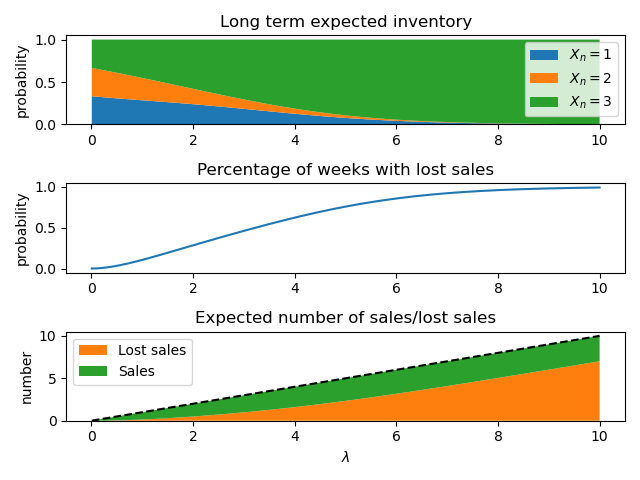
\includegraphics[width=200pt]{images/aquarium.png}
\end{center}

Observe how the number of sales converges to $3$ as $\lambda \to \infty$, which makes sense since that is the maximum inventory. The more clients that come to the store, the more likely to sell all the inventory every week.


	
\end{slide}

\end{solution}



\begin{slide}
\question

Construct a Markov chain model for the heat equation interpreting it as particles randomly bumping around and averaging their temperature when they meet.

	
\end{slide}




\begin{slide}
\question
\begin{problem}[Stochastic Simulation]
It is very rare to be able to obtain analytic results for probabilistic models, so we will study simulating them.
\end{problem}

\SavedDefinitionRender{discrete-event}

\SavedDefinitionRender{tau-leaping}

Here is some code simulating an Exponential Distribution using each method.
\begin{itemize}
	\item \href{https://utoronto.syzygy.ca/jupyter/user-redirect/git-pull?repo=https://github.com/bigfatbernie/IBLMathModeling&subPath=book/python/numerical-stochastic.ipynb}{\tt numerical-stochastic.ipynb}
\end{itemize}

	
\end{slide}



\begin{slide}
\question \label{aquarium2}

Recall Exercise \ref{aquarium}. 

\begin{parts}
	\item Using the Jupyter Notebook 	\href{https://utoronto.syzygy.ca/jupyter/user-redirect/git-pull?repo=https://github.com/bigfatbernie/IBLMathModeling&subPath=book/python/aquarium-part2.ipynb}{\tt aquarium-MonteCarlo.ipynb}, simulate the aquarium problem.

	\item The store is considering an alternative re-stocking policy: when the stock is down to 1 aquarium, they flip a coin and decide whether to re-stock to 3 aquariums or not.
	
	Simulate this new store policy in the same Jupyter Notebook and compare the results.
	
	\item Run the last part of the Jupyter Notebook to combine the results of these two policies. You need to add titles and legends to the graphs, and labels to the $x-$ and $y-$ axes. Compare the results.

	\item \label{aquarium2:economic} Create an economic model for the store that includes: profit from each aquarium sale, stocking cost per aquarium in stock, shipping cost when re-ordering new aquariums.
	
		Evaluate which of the previous two policies is better. 
\end{parts}

\end{slide}


\begin{solution}
\begin{slide}
Solution python: \href{https://utoronto.syzygy.ca/jupyter/user-redirect/git-pull?repo=https://github.com/bigfatbernie/IBLMathModeling&subPath=book/python/aquarium-MonteCarlo-sol.ipynb}{\tt aquarium-MonteCarlo-sol.ipynb}

\begin{parts}	
	\item Plot one simulation for the original re-stocking policy.
	
		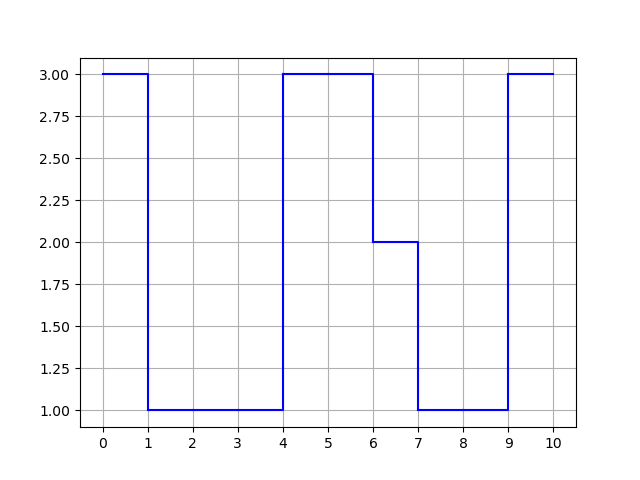
\includegraphics[width=0.4\textwidth]{images/aquarium-sim-og.png}
	\item Plot the same simulation for the modified re-stocking policy.
	
		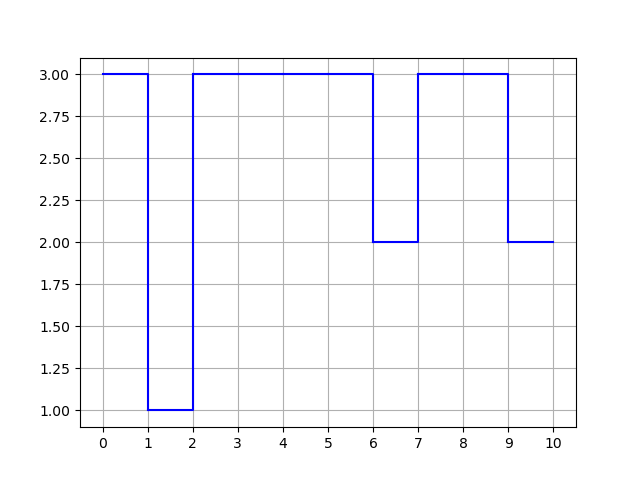
\includegraphics[width=0.4\textwidth]{images/aquarium-sim-mod.png}
		
		
	Observations:
	\begin{itemize}
		\item Week 1: the modified store decided not to order new aquariums, even though they only had 1 in stock
		\item Week 2: the modified store re-stocked
		\item Week 3: the original store had 1 aquarium in stock and sold it, then re-stocked
		\item Week 3: the modified store, had 3 aquariums in stock and sold at least 2, because they also re-stocked
		\item Week 3: This means that the original store lost 1 or 2 more sales than the modified store.
	\end{itemize}	
	
	
	\item From the plots below, we can see that the modified store loses much fewer sales.
\end{parts}	

		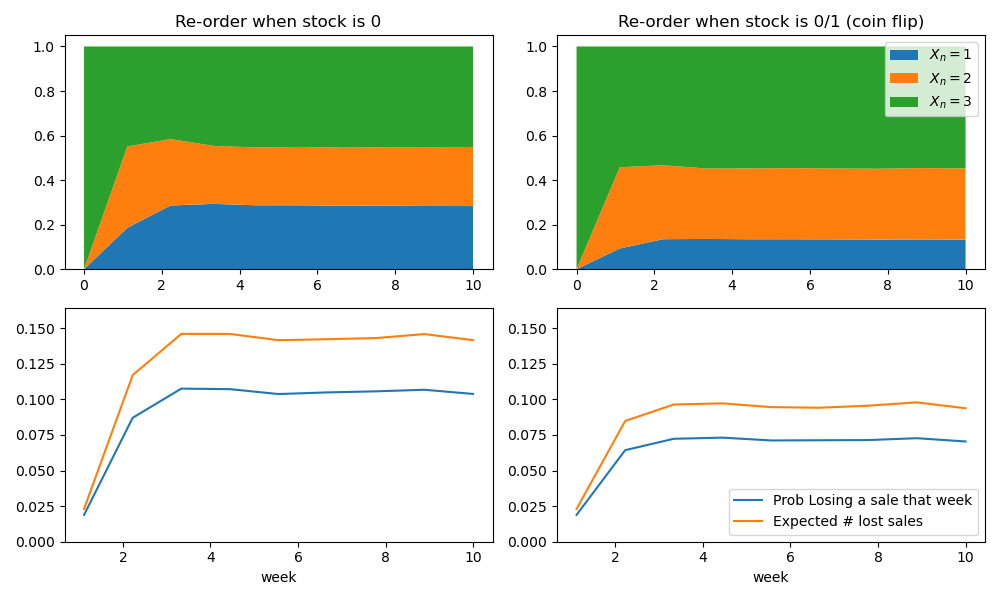
\includegraphics[width=0.75\textwidth]{images/aquarium-sim.png}
	

\end{slide}
	
\end{solution}



\begin{slide}
\question \label{SIR_stochastic}
	
Recall the SIR model:
\begin{align*}
\frac{dS}{dt} 	& = - \beta SI \\
\frac{dI}{dt} & = \beta SI - \gamma I \\
\frac{dR}{dt} & = \gamma I
\end{align*}

We now want to create a stochastic simulation for the same model:
\begin{itemize}
	\item A \textit{susceptible} individual becomes \textit{infected} with probability $\beta I$ per unit time;
	\item An \textit{infected} individual becomes \textit{recovered} with probability $\gamma$ per unit time.
\end{itemize}

An \textit{event} happens when one of these two changes of circumstances happens and we assume that the time between events is \textit{memoryless}, hence it should be \textit{exponentially} distributed with the appropriate rate.

Since the number of infected individuals changes with every event, the rate will need to be updated with each event.

\begin{parts}
	\item Explain why the \textit{discrete event} method will give a better approximation than the  \textit{$\tau$-leaping} method.
	\item We are expecting lots of events, so we will use the $\tau$-leaping method.
		we use the binomial distribution (the discrete version of the Poisson distribution) to determine whether an individual became infected or not.
		Then complete the following for \textbf{one time step} of length $\Delta t$:
		\begin{itemize}
			\item $\Pr($new infectives$=k)\quad =\quad $
			\item $\Pr($new recovereds$=k)\quad =\quad $
		\end{itemize}
	\item Create a simulation for $t\in [0,10]$ and $\Delta t = 0.1$ with:
	\begin{itemize}
		\item Initial population: $S_0=99$, $I_0=1$, $R_0=0$
		\item Infection rate: $\beta=0.1$ (which means $R_0=10$)
		\item Recovery rate: $\gamma =1$
	\end{itemize}
	\item Compare the differences with the deterministic continuous model.
\end{parts}

\end{slide}


\begin{solution}
\begin{slide}
\begin{parts}
	\item With the \textit{discrete event} method, we recalculate the rates with every event, but with the \textit{$\tau$-leaping} method, we don't, we calculate how many events happen in a predetermined timestep size. Since in this model, the rate changes with each event, the discrete event method is more accurate.

	\item 

		$\Pr($new infectives$=k)\quad =\quad {{S}\choose{k}} (\Delta t \beta I)^k (1-\Delta t \beta I)^{S-k}$
		
		$\Pr($new recovereds$=k)\quad =\quad {{I}\choose{k}} (\Delta t \gamma)^k (1-\Delta t \gamma)^{I-k}$

		
	\item The first graph is the result of 10 simulations with \href{https://utoronto.syzygy.ca/jupyter/user-redirect/git-pull?repo=https://github.com/bigfatbernie/IBLMathModeling&subPath=book/python/SIR-stochastic-sol.ipynb}{\tt SIR-stochastic-sol.ipynb}
	
	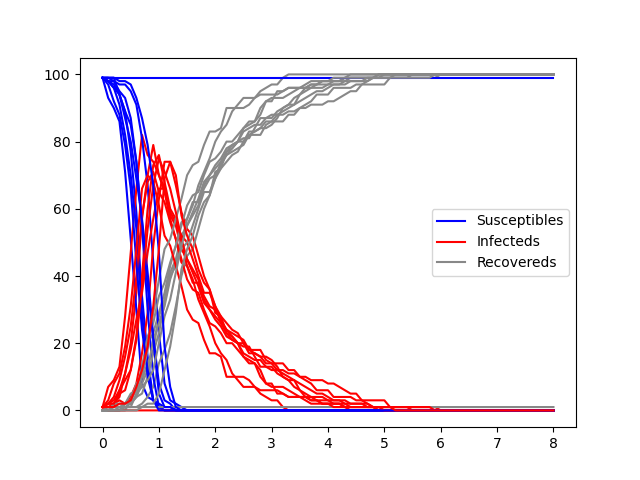
\includegraphics[width=0.5\textwidth]{images/SIR-stochastic1.png}

	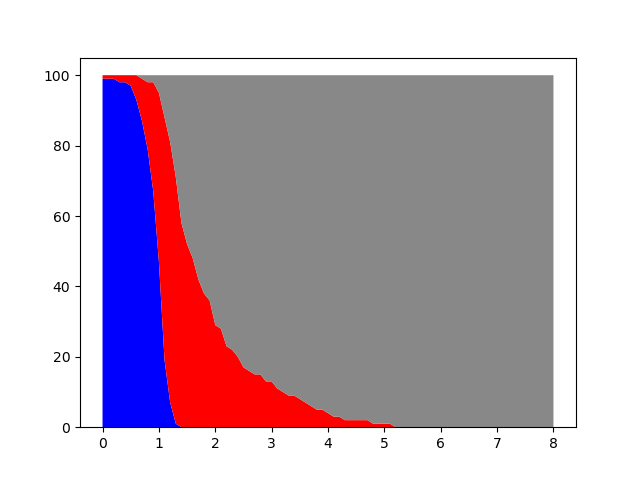
\includegraphics[width=0.5\textwidth]{images/SIR-stochastic2.png}
	
	\item Observe how on one of the simulations, no one else became infected, which would not be possible on the continuous model. Also note that the infected population actually becomes zero in finite time as opposed to asymptotically converging to 0 in the continuous model.
\end{parts}
	
\end{slide}
	
\end{solution}



\begin{slide}
\question

\textbf{Monte Carlo Simulations} and their accuracy.

The simulations we have done with the aquarium and SIR models are called Monte Carlo simulations. These rely on running the simulations again and again, which can take a long time. To compare the accuracy with other numerical methods:

\begin{itemize}
	\item Monte Carlo has square-root convergence: To be 2x more accurate, we need to run it 4x more
	\item Euler has linear convergence: To be $2^1$x more accurate, we need to run it 2x more
	\item Runge-Kutta 4 has 4th order convergence: To be $2^4$x more accurate, we need to run it 2x more
\end{itemize}

They can be very convenient though to run through examples and try different strategies, e.g. for the aquarium store, changing the re-stocking policy required 1-2 different lines of coding.

\end{slide}


\begin{slide}
\question

\begin{problem}[Optimization with Stochastic Simulation]

We want to continue on the idea of Exercise \ref{aquarium2}.\ref{aquarium2:economic}.

We assume the following:
\begin{enumerate}
	\item Each delivery has a cost \$$d$ independent of the number of aquariums shipped.
	\item Each sale has a profit of \$$s$.
	\item Each item in inventory has a small probability $\rho$ of being damaged during the week and that would incur as a cost of \$$c$. The aquariums are damaged independently, so the number of damaged aquariums is binomial $K \sim B(X_n,\rho)$.
\end{enumerate}

We want to optimize the profit.
\end{problem}

\begin{slidesonly}
\vspace{2cm}	
\end{slidesonly}


\begin{parts}
	\item What is the formula for the profit on week $n$ with inventory $X_n$ and demand $D_n$?
	\item Let policy $p(x)$ be the number of aquariums that are reordered when there $x$ aquariums in stock. What are all the possible values $p(x)$? How many possible policies are there?
	\item If the store had a maximum of $m$ aquariums in stock (instead of 3), how many different policies are there?
	\item We can reduce these numbers, because the cost of ordering new aquariums is fixed and doesn't depend on how many aquariums are ordered. 
		
		So if we're willing to re-order to a certain stock $L$ when  the stock is $x$: $p(x) = $?
		then for $y<x$, we should have $p(y)= $?
	
	\item Based on the previous property, how many policies are there for a maximum of $m$ aquariums?
	
\end{parts}

	
\end{slide}



\begin{solution}
\begin{slide}
\begin{parts}
	\item We now have 
	\[
	R_n = \begin{cases}
		s\cdot \min\{D_n,X_n\} - d - c \cdot K_n & \text{if} \min\{D_n,X_n\}>0 \\
		- c \cdot K_n & \text{otherwise}
 	\end{cases}
	\]

	\item $p(3) = 0$, $p(2)\in\{0,1\}$, $p(1)\in\{0,1,2\}$, $p(0)\in\{0,1,2,3\}$, with a total number of possible policies of $4!$.

	\item If the maximum is $m$ aquariums, then there are $(m+1)!$ possible policies, which quickly become too many to check.

	\item So if we're willing to re-order to a certain stock $L$ when  the stock is $x$: $p(x) = L-x$
		then for $y<x$, we should have $p(y)= L-y$?

	\item So we have:
	\[ 
	p(x) = \begin{cases}
			\max\{L-x,0\}	& \text{ if } x < t 	 \\
			0 				& \text{ if } x \geq t 	
		 \end{cases}
	\]
	where $t$ is the level below which the store restocks and $L$ is the level it tries to achieve.

	The possible cases are: $t \in \{1, \ldots, m\}$ and $L \in \{t, \ldots, m\}$, so there are
	\[\sum_{t=1}^m (m-t+1) =\frac12 m(m+1).
	\]
\end{parts}
\end{slide}	
\end{solution}


\begin{slide}
\SavedDefinitionRender{WelfordAlgorithm}


We can now estimate the long term profit by simulating the Markov decision process for each policy.

\begin{itemize}
	\item We can reduce the sampling error by simulating for a large number of weeks (instead of simulating several times).
	\item We can use Welford's algorithm to estimate the mean weekly profit and its variance.
	\item Even though Welford's algorithm reduces the computations needed to calculate the mean and variance, we still need to run the simulation for each possible policy and each week.
\end{itemize}

\begin{parts}
\setcounter{partsitem}{4}
	\item Use Welford's algorithm to calculate all mean and variance of the profit for all the possible policies with $m=3$ (the original setting).
	Use the following values: 
	\begin{itemize}
		\item $\lambda=1$ expected customer per week
		\item Delivery cost $d=\$5$ and sale profit $s=\$20$
		\item Damage probability $\rho=0.01$ and cost $c=\$60$
	\end{itemize}
	
	What is the best policy?
\end{parts}	
	
\end{slide}


\begin{solution}
\begin{slide}
\begin{parts}
\setcounter{partsitem}{4}
	\item Running $1\,000\,000$ weeks and ignoring the first 50 weeks over all 6 policies, we obtain the best policy: 
	\begin{itemize}
		\item \textit{Re-order if the stock $X=0$ or $X=1$.}
		\item The average weekly profit is \$ 15.28
		\item The standard deviation is \$ 20.38
	\end{itemize}
	Below is a graph of the average profits and their standard deviations for each re-stocking policy.
	
	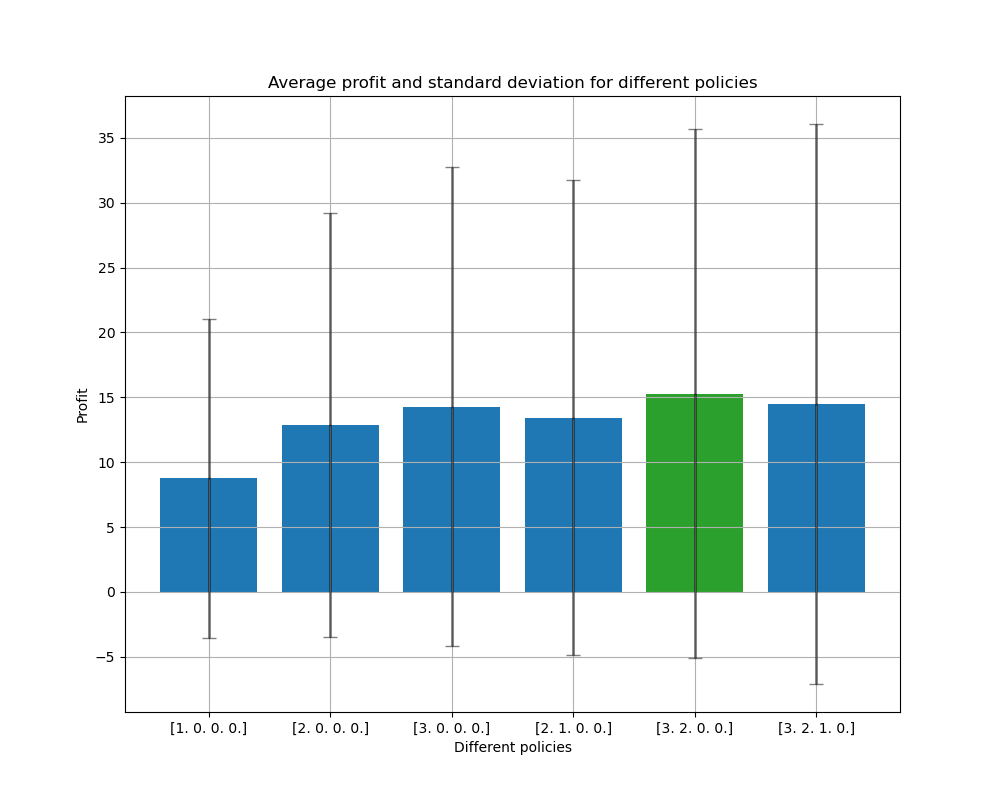
\includegraphics[width=0.5\textwidth]{images/aquarium-policies.png}	

	Code: \href{https://utoronto.syzygy.ca/jupyter/user-redirect/git-pull?repo=https://github.com/bigfatbernie/IBLMathModeling&subPath=book/python/aquarium-MC-policies-sol.ipynb}{\tt aquarium-MC-policies-sol.ipynb}
	
	
\end{parts}


	
\end{slide}	
\end{solution}




\begin{slide}
\question

\SavedDefinitionRender{Q-learning}

\end{slide}

\begin{slide}
Let us now implement the Q-learning algorithm to calculate the optimal policies for different cases.

\begin{parts}
	\item Use \href{https://utoronto.syzygy.ca/jupyter/user-redirect/git-pull?repo=https://github.com/bigfatbernie/IBLMathModeling&subPath=book/python/aquarium-Qlearn.ipynb}{\tt aquarium-Qlearn.ipynb} to calculate the quality of state matrix $Q$ for the original case $m=3$, $\rho=0.01$.
	\item Use this to deduce the best policy in this case.
	\item Use the same process to deduce the optimal policies for the cases $m \in \{1, \ldots 7\}$ and $\rho \in \{0.01, 0.03, 0.05\}$.
\end{parts}
\end{slide}



\begin{solution}
\begin{slide}
\begin{parts}
	\item We obtain the matrix
	\[ 
	Q = \mat{
		83.98925114 & 91.15973818 & 95.97324719 & \pmb{99.00385354} \\
		96.15340924 & 96.03440076 & \pmb{98.52386915} &  0. \\
		\pmb{101.72981334} & 98.57852473 &  0.         &  0. \\
		\pmb{104.05899297} &  0.         &  0.         &  0.
	}
	\]
	
	\item To deduce the best policy:
	\begin{itemize}
		\item We need to find the value of $a$ that maximizes the quality for each state
		\item We need to find the maximum for each row and identify the value of that column
	\end{itemize} 
	
	For $m=3$ and $\rho=0.01$, we get:
	\begin{itemize}
		\item 3 \quad 2 \quad 0 \quad 0
	\end{itemize}
	which means that the store should order 3 aquariums when inventory is 0, 2 aquariums when inventory is 1, and not re-stock otherwise.
	
	This matches our previous conclusions.
	
\end{parts}
\end{slide}

\begin{slide}
\begin{parts}
\setcounter{partsitem}{2}
	\item Here are my results:
\end{parts}
	
	\begin{tabular}{|l|l|l|l|}
	\hline
	$\pmb{m}$ & \textbf{policy for $\pmb{\rho=0.01}$}
		& \textbf{policy for $\pmb{\rho=0.03}$}
		& \textbf{policy for $\pmb{\rho=0.05}$} \\ \hline
	\textbf{1} 
		& 1 \quad 0 
		& 1 \quad 0 
		& 1 \quad 0 \\
	\textbf{2} 
		& 2 \quad 1 \quad 0 
		& 2 \quad 0 \quad 0 
		& 2 \quad 0 \quad 0 \\
	\textbf{3} 
		& 3 \quad 2 \quad 0 \quad 0 
		& 3 \quad 2 \quad 0 \quad 0 
		& 2 \quad 0 \quad 0 \quad 0 \\
	\textbf{4} 
		& 4 \quad 3 \quad 0 \quad 0 \quad 0 
		& 3 \quad 2 \quad 0 \quad 0 \quad 0 
		& 2 \quad 0 \quad 0 \quad 0 \quad 0 \\
	\textbf{5}
		& 5 \quad 4 \quad 0 \quad 0 \quad 0 \quad 0 
		& 3 \quad 2 \quad 0 \quad 0 \quad 0 \quad 0 
		& 2 \quad 0 \quad 0 \quad 0 \quad 0 \quad 0 \\
	\textbf{6}
		& 4 \quad 4 \quad 0 \quad 0 \quad 0 \quad 0 \quad 0 
		& 3 \quad 2 \quad 0 \quad 0 \quad 0 \quad 0 \quad 0 
		& 2 \quad 0 \quad 0 \quad 0 \quad 0 \quad 0 \quad 0 \\
	\textbf{7}
		& 5 \quad 4 \quad 0 \quad 0 \quad 0 \quad 0 \quad 0 \quad 0 
		& 3 \quad 2 \quad 0 \quad 0 \quad 0 \quad 0 \quad 0 \quad 0
		& 2 \quad 0 \quad 0 \quad 0 \quad 0 \quad 0 \quad 0 \quad 0\\
	\hline	
	\end{tabular}	

Observe that because the Q-learning algorithm moves randomly from state to state and explores random actions $a$ each iteration, the more possible states and actions, the \textit{weeks} we need and the results are less conclusive.

After running the simulation a few times for $m=6,7$ and $\rho=0.01$, the results varied between these policies:
\begin{itemize}
	\item $4 \quad 4 \quad 0 \quad \cdots$
	\item $5 \quad 4 \quad 0 \quad \cdots$
	\item $6 \quad 4 \quad 0 \quad \cdots$
\end{itemize}

\end{slide}	
\end{solution}













\begin{bookonly}
%\begin{appendix}\label{APPSLEI}
%	\Title{Systems of Linear Equations I}
%
%	In this appendix you will learn
%	\begin{itemize}
%		\item What a system of linear equations is.
%		\item What the solution set to a system of equations is, and what it means for a system of equations
%			to be consistent or inconsistent.
%		\item How augmented matrices can be used to solve systems of linear equations.
%		\item How to apply row reduction to find a unique solution to a system of linear
%			equations and to determine if a system of linear equations is consistent or inconsistent.
%	\end{itemize}
%
%		An \emph{equation} encodes a relationship between quantities. For
	example, writing
	\[
		\underbrace{\text{Slices of cake}}_C = \underbrace{\text{Slices you ate}}_M + \underbrace{\text{Slices your brother ate}}_B
	\]
	specifies a precise relationship between the quantities $C$, $M$, and $B$. 
	Without more information, $C$, $M$, and $B$ could be almost anything. As such, we call 
	$C$, $M$, and $B$
	\emph{variables} or \emph{unknowns}. 
	However, the
	relationship \emph{between} them is precisely defined. 

	Additional relationships give rise to additional equations, which we express concisely as a
	\emph{system of equations}, that is, a list of equations. For example, suppose you know the cake
	had six pieces and your brother ate twice as many pieces as you. We might now write the system
 
	\begin{align*}
  		C &= M + B \\
  		B &= 2M \\
  		C &= 6
	\end{align*}
 
	which should be interpreted as: ``the relationship $C=M+B$ holds \emph{and} the relationship $B=2M$ holds \emph{and}
	the relationship $C=6$ holds.''
	All this information, taken together, is enough to deduce the unknowns: $M=2$, $B=4$, and $C=6$.

	Systems of equations naturally appear in linear algebra through vector equations. Suppose $\vec u=\mat{1\\2}$, $\vec v=\mat{2\\3}$,
	and $\vec w=\mat{1\\1}$. You might wonder if $\vec w$ was a linear combination of $\vec u$ and $\vec v$. The answer is \emph{yes} if and
	only if the vector equation
	\[
		\vec w=a\vec u+b\vec v
	\]
	has a solution for some $a$ and $b$. Written in coordinates, this equation is equivalent to
	\[
		\mat{1\\1}=a\mat{1\\2}+b\mat{2\\3} = \mat{a+2b\\2a+3b}.
	\]
	Equating coordinates, a system of equations appears:
	\[
		\systeme{a+2b=1,2a+3b=1}
	\]

	Every vector equation, by way of coordinates, corresponds to a system of equations. And, fortunately for us, there is
	an \emph{algorithm} to find all solutions to these systems\footnote{ Saying there is an \emph{algorithm} for ``$X$''
	means that there is a specific set of (non-random) rules that \emph{always} accomplishes ``$X$''. As a consequence, doing
	``$X$'' never requires special insight. For example, there \emph{is} an algorithm for multiplying numbers, but there \emph{is not}
	an algorithm for factoring polynomials of degree 5 or greater.}.

	\Heading{Systems of Linear Equations}

	There's no guarantee that a general equation, like $x^4-e^x+7=0$, has a solution, and it might
	be impossible to decide if an arbitrary equation has a solution, let alone what the solutions 
	are!\footnote{ Fermat's Last Theorem famously claimed that $a^n+b^n=c^n$
	has no positive integer solutions for $n\geq 3$. However, it took 350 years of human ingenuity before anyone was able rigorously
	back up the claim.} However, for \emph{linear} equations and systems of linear equations we can \emph{always} tell
	whether there is a solution and what the solution(s) are.
	
	\begin{definition}[Linear Equation]
		A \emph{linear equation} in the variables $x_1,\ldots,x_n$ is one that can be expressed
		as
		\[
			a_1x_1+a_2x_2+\cdots+a_nx_n=c
		\]
		for constants $a_1,\ldots, a_n$ and $c$. A \emph{system of linear equations} is a system of equations 
		consisting of one or more linear equations.
	\end{definition}

	Every vector equation corresponds to an \emph{equivalent} system of linear equations and vice versa, where equivalent
	means ``expresses the same relationships between variables''.

	\begin{example}
		Write down the vector equation corresponding to the system of linear equations $\systeme{2x+3y+z=2,y-z=-1}$
		and the system of linear equations corresponding to the vector equation $t\vec w+\vec u=r\vec v$ where $\vec w=\mat{1\\-1}$, $\vec u=\mat{2\\3}$,
		and $\vec v=\mat{4\\4}$.

		The system $\systeme{2x+3y+z=2,0x+y-z=-1}$ corresponds to the vector equation
		\[
			x\mat{2\\0} + y\mat{3\\1} + z\mat{1\\-1} = \mat{2\\-1}.
		\]
		
		As for the vector equation $t\vec w+\vec u=r\vec v$, rewriting each vector in coordinates gives us a corresponding system of linear equations:
		\begin{align*}
			t\vec w + \vec u = r\vec v
			\rightarrow
			t\mat{1\\-1} + \mat{2\\3} &= r\mat{4\\4}\\
			\mat{t+2\\-t+3} &= \mat{4r\\4r}
			\rightarrow
			\systeme{t-4r=-2, -t-4r=-3}.
		\end{align*}
	\end{example}

	\begin{emphbox}[Takeaway]
		Every vector equation corresponds to a system of linear equations and every system of linear equations
		corresponds to a vector equation.
	\end{emphbox}

	\Heading{Solution Sets}

	Before looking at how to solve systems of linear equations, let's agree on some terminology.

	A \emph{solution} to an equation is a particular choice of values for the variables that satisfy (i.e. make true)
	the equation. For example
	\begin{equation}
		\label{SOLNSETEXAMPLE}
		x+y=4
	\end{equation}
	has a solution $x=y=2$. However, $x=y=2$ is just one of \emph{many} possible solutions; we also have $x=4$ and $y=0$ or $x=-2$ and
	$y=6$. The \emph{solution set},
	also called the \emph{complete solution}, to an equation (or system of equations) is the set of all possible solutions.
	For example, the solution set to Equation \eqref{SOLNSETEXAMPLE} is $S=\Set{(x,y)\given y=4-x}$. %=\Set{(t,4-t)\given a\in \R}$.
	In this case, $S$ contains infinitely many solutions, including $(x,y)=(2,2)$, the first solution we found.

	Solution sets look a lot like sets of vectors: the set $S=\Set{(x,y)\given y=4-x}$ could be thought of as a subset of $\R^2$
	where we identify a solution $x=a$ and $y=b$ with the column vector $\mat{a\\b}$. Drawing $S$ as a subset of $\R^2$, we see a familiar
	picture.

	\begin{center}
		\begin{tikzpicture}
			\begin{axis}[
				anchor=origin,
				disabledatascaling,
				xmin=0,xmax=5,
				ymin=0,ymax=5,
				xtick={-1,...,5},
				ytick={-1,...,5},
				x=1cm,y=1cm,
				grid=both,
				grid style={line width=.1pt, draw=gray!10},
				axis lines=middle,
				minor tick num=0,
				enlargelimits={abs=0.5},
				axis line style={latex-latex},
				ticklabel style={font=\tiny,fill=white},
				xlabel style={at={(ticklabel* cs:1)},anchor=north west},
				ylabel style={at={(ticklabel* cs:1)},anchor=south west}
			]
				\draw [mygreen, thick] (-2,6) -- (6,-2);
			\end{axis}
		\end{tikzpicture}
	\end{center}

	It's the graph of the line given in $y=mx+b$ form by $y=-x+4$. In other words, \emph{via solution sets, equations and systems
	of equations can represent geometric objects.}

%	\medskip
%	If this all seems straightforward, great! Since grade school you've been training to apply algebra to geometry problems
%	and vice versa\footnote{ It was a big deal when equations saw their first applications to geometry and it is by no means
%	an obvious idea! If you're interested, look up the history of \emph{analytic geometry}, which is the formal name for what
%	we're doing.}. However, we need to take special care to note the assumptions we've made. After all, it would be
%	perfectly reasonable to claim that $S'=\Set{(y,x)\given y=4-x}$ (note the difference between $S$ and $S'$) 
%	is the solution set to Equation \eqref{SOLNSETEXAMPLE}.
%	However, it becomes less clear how $S'$ should be interpreted as a subset of $\R^2$. Should $(y,x)=(a,b)$ correspond to the
%	column vector $\mat{a\\b}$ or is $\mat{b\\a}$ the correct column vector? To solve this issue, we use the following convention.
%
%	\begin{emphbox}[Solution Set Convention] Unless otherwise specified,
%		solutions are converted to column vectors based on the order the variables are specified
%		in the original equations. This order will almost always be alphabetical if variables are assigned
%		different letters (e.g, $x$, $y$, $z$) or numerically if variables are indexed (e.g., $x_1$, $x_2$, $x_3$).
%	\end{emphbox}
%
%	Following this convention, $S$ is the ``correct'' solution set. That is, without specifying otherwise, the solutions
%	to $x+y=4$ correspond to the set $\Set*{\mat{a\\b}\given b=4-a}\subseteq \R^2$. This just so happens to agree with grade-school
%	convention\footnote{ It's as if there's a vast underworld of educators who plan how math should be taught from the time you
%	were five up until now.}.

	\Heading{Consistent \& Inconsistent Systems}

	Consider the following equations (as separate equations, not as a system):
	\[
		x^2=0\qquad\text{with solution set}\qquad S_x\subseteq \R,
	\]
	\[
		y^2=4\qquad\text{with solution set}\qquad S_y\subseteq \R,
	\]
	and
	\[
		z^2=-1\qquad\text{with solution set}\qquad S_z\subseteq \R.
	\]
	$S_x=\Set{0}$ consists of a single number. $S_y=\Set{2,-2}$ consists of two numbers, and $S_z=\Set{}$ consists of no
	numbers\footnote{ We're not allowing complex numbers at the moment.}.
	In this case, we would call the first two equations \emph{consistent} and the third equation \emph{inconsistent}.

	\begin{definition}[Consistent \& Inconsistent]
		An equation or system of equations is called \emph{consistent} if it has at least one solution. That
		is, its solution set is non-empty. Otherwise, an equation or system of equations is called \emph{inconsistent}.
	\end{definition}

	Why the word \emph{consistent}? This comes from the term \emph{logically consistent} which means ``able to be true''.
	An equation is an assertion that the left hand side equals the right hand side. If that can never happen, the assertion
	is not logically consistent.

	This terminology becomes more clear with systems. Consider the system
	\[
		\systeme{x-y=0,x-y=1}.
	\]
	From the first equation, we deduce $y=x$. From the second equation, we deduce $x=1+y$. Since $x=x$, we know that
	$y=x=1+y$ and therefore
	$y=1+y$. However, this is never true! There is a logical inconsistency between the two equations. In isolation they're
	fine, but taken together they're not.

	\Heading{Equivalent Systems}
	Two systems of equations are logically equivalent if they express the same relationships
	between their variables. For example, the equations $x=2y$ and $\tfrac{1}{2}x=y$ express the exact same
	relationship between the variables $x$ and $y$. This can be formalized using solution sets.

	\begin{definition}[Equivalent Systems]
		Two equations or systems of equations are called \emph{equivalent}\index[definitions]{Equivalent systems} if they have the same solution sets.
	\end{definition}

	Again, $x=2y$ and $\tfrac{1}{2}x=y$ both have the same solution set (a line through the origin of slope $\tfrac{1}{2}$),
	and so they are equivalent.

	Philosophical note: the process of ``doing algebra'' can be viewed as
	the process of \emph{manipulating equations/systems into easier to understand equivalent 
	equations/systems}. When you're asked to algebraically solve $x^2-4=0$. You might first factor to get the 
	equivalent equation $(x-2)(x+2)=0$. Then, since non-zero numbers cannot multiply to give zero, we know
	$x-2=0$ or $x+2=0$, which in turn is equivalent to $x=\pm2$. It's always been about equivalent systems!\footnote{
	Technically, up to this point we've been talking about \emph{conjunctive} systems, which means that a solution
	must hold for all equations of a system. The system $x=\pm 2$ is a \emph{disjunctive} system, which means a solution
	only needs to hold for \emph{one} of the equations ($x=2$ or $x=-2$), but the idea is the same.}

	\Heading{Row Reduction}

	Consider the vector equation
	\[
		t\vec u+s\vec v+r\vec w = \vec p\qquad\text{where}\qquad \vec u=\mat{1\\2\\1},\ 
		\vec v=\mat{2\\1\\-4},\ \vec w=\mat{-2\\-5\\1},\ \vec p=\mat{-15\\-21\\18}.
	\]
	By expanding in terms of coordinates, we get an equivalent system of linear equations.
	\begin{equation}
		\label{EQVECEQ2}
		\systeme[tsr]{
			t+2s-2r=-15@\qquad\text{row}_1,
			2t+s-5r=-21@\qquad\text{row}_2,
			t-4s+r=18@\qquad\text{row}_3
		}
	\end{equation}

	The most general way to solve any system is by \emph{substitution}. For System 
	\eqref{EQVECEQ2}, we could solve the first equation for $t$, substitute the result in
	the remaining equations, solve the next equation for $s$, etc.. However,
	because System \eqref{EQVECEQ2} is a \emph{linear} system, there's an alternate
	method: \emph{row reduction}\footnote{
	Row reduction is sometimes referred to as \emph{Gaussian elimination},
	\emph{Gauss-Jordan elimination}, or just \emph{elimination}; though there are subtle differences between Gaussian
	and Gauss-Jordan elimination,
	they aren't important, and we'll refer to all similar methods as \emph{row reduction}.}.

	Study the following manipulations of System \eqref{EQVECEQ2} and convince yourself
	that each operation produces a system equivalent to the one it came from.
	\begin{align}
	\sysdelim\{.
		\systeme[tsr]{
			t+2s-2r=-15,
			2t+s-5r=-21,
			t-4s+r=18
		}
		&\xrightarrow{\text{row}_3\mapsto\text{row}_3-\text{row}_1}
	\sysdelim\{.
		\systeme[tsr]{
			t+2s-2r=-15,
			2t+s-5r=-21,
			-6s+3r=33
		}\nonumber\\[4pt]
		&\xrightarrow{\text{row}_2\mapsto\text{row}_2-2\text{row}_1}
	\sysdelim\{.
		\systeme[tsr]{
			t+2s-2r=-15,
			-3s-r=9,
			-6s+3r=33
		}\nonumber\\[4pt]
		&\xrightarrow{\text{row}_3\mapsto\text{row}_3-2\text{row}_2}
	\sysdelim\{.
		\systeme[tsr]{
			t+2s-2r=-15,
			-3s-r=9,
			  5r=15
		}\label{EQEQUIVSYS}
	\end{align}
	From the final system, System \eqref{EQEQUIVSYS}, it's easy to see that $r=3$.
	From there,
	we can substitute $r=3$ into the second row of System \eqref{EQEQUIVSYS}
	to find $s=-4$ and we can substitute both $r$ and $s$ into the first row of System \eqref{EQEQUIVSYS}
	to find $t=-1$.

	By adding and subtracting rows, we ``reduced'' the number of variables from some equations until
	they were easy to solve. As an added benefit, every system along the way to System \eqref{EQEQUIVSYS}
	was nicely organized and formatted. In fact, the systems are so well organized that we can
	save time by not writing the variables and keeping track of the numbers in an \emph{augmented matrix}\footnote{
		A \emph{matrix} is a box of numbers. An \emph{augmented matrix} is a matrix with
		extra information associated with it.
	}. That is, instead of writing
	\[
		\systeme[tsr]{
			t+2s-2r=-15,
			2t+s-5r=-21,
			t-4s+r=18
		}
	\]
	we will write
	\[
		\begin{bmatrix}[rrr|r]
			1&2&-2 & -15\\
			2&1&-5&-21\\
			1&-4&1&18
		\end{bmatrix}.
	\]
	We call the matrix an \emph{augmented matrix} to stress that it contains two types of information:
	the \emph{coefficients} of the variables $t$, $s$, and $r$ and the \emph{constants} on
	the right hand side of the equations. An (optional) vertical line
	separates the two types of numbers.


	Now, the process of row reduction looks like this:
	\begin{align*}
		{\footnotesize
		\systeme[tsr]{
			t+2s-2r=-15,
			2t+s-5r=-21,
			t-4s+r=18
		}
		} \rightarrow
		\begin{bmatrix}[rrr|r]
			1&2&-2 & -15\\
			2&1&-5&-21\\
			1&-4&1&18
		\end{bmatrix}
		&\xrightarrow{\text{row}_3\mapsto\text{row}_3-\text{row}_1}
		\begin{bmatrix}[rrr|r]
			1&2&-2 & -15\\
			2&1&-5&-21\\
			0&-6&3&33
		\end{bmatrix}\\
		&\xrightarrow{\text{row}_2\mapsto\text{row}_2-2\text{row}_1}
		\begin{bmatrix}[rrr|r]
			1&2&-2 & -15\\
			0&-3&-1&9\\
			0&-6&3&33
		\end{bmatrix}\\
		&\xrightarrow{\text{row}_3\mapsto\text{row}_3-2\text{row}_2}
		\begin{bmatrix}[rrr|r]
			1&2&-2 & -15\\
			0&-3&-1&9\\
			0&0&5&15
		\end{bmatrix}
		\rightarrow
		{\footnotesize
			\systeme[tsr]{
			t+2s-2r=-15,
			-3s-r=9,
			  5r=15
			}
		}
	\end{align*}

	The operations are identical, but we write augmented matrices instead of equations.

	\begin{emphbox}[Takeaway]
		Augmented matrices are a notational tool that makes the process of doing row reduction more efficient.
	\end{emphbox}

	\Heading{The Rules of Row Reduction}

	So far, we've been able to row reduce systems by adding a multiple of one row to another\footnote{ Technically, we subtracted, but
	that's just adding a negative.}, but to fully solve \emph{any} system, we need additional operations\footnote{ If you're clever,
	you can think up alternatives to the elementary row operations that work just as well, but there's good reason to favor 
	the
	three elementary row operations. We'll see them when discussing matrix decompositions.}.
	\begin{definition}[Elementary Row Operations]
		The three \emph{elementary row operations}, which can be performed on a matrix or system of equations, are
		\smallskip
		\begin{itemize}
			\item swapping two rows (written $\text{row}_i\leftrightarrow \text{row}_j$),
			\item multiplying a row by a non-zero scalar (written $\text{row}_i\mapsto k\,\text{row}_i$), and
			\item adding a multiple of one row to another (written $\text{row}_i\mapsto \text{row}_i+ k\,\text{row}_j$).
		\end{itemize}
	\end{definition}

	Notice that each elementary row operation can be undone. For example, if you perform $\text{row}_i\mapsto k\,\text{row}_i$,
	you can undo it with $\text{row}_i\mapsto \tfrac{1}{k}\,\text{row}_i$. Therefore, applying an elementary row operation
	to a system is guaranteed to
	produce an equivalent system. 

	The strategy for solving a system is now summarized as:
	\begin{enumerate}
		\item Rewrite the system as an augmented matrix.
		\item Use elementary row operations to zero-out the lower triangle of the augmented matrix.
		\item Convert the matrix back to a system of equations.
		\item Read off the solution (substituting when necessary).
	\end{enumerate}

	\begin{example}
		Find a solution to the following system:
		\[
			\systeme{
				a+3b+2c=1,
				2a+7b+5c=2,
				-a-4b=11
			}.
		\]

		To do so, we rewrite the system as an augmented matrix then row reduce.
		\begin{align*}
			{\footnotesize
			\systeme{
				a+3b+2c=1,
				2a+7b+5c=2,
				-a-4b=11
			}
			} \rightarrow
			\begin{bmatrix}[rrr|r]
				1&3&2 & 1\\
				2&7&5 & 2\\
				-1&-4&0 & 11
			\end{bmatrix}
			&\xrightarrow{\text{row}_2\mapsto\text{row}_2-2\text{row}_1}
			\begin{bmatrix}[rrr|r]
				1&3&2 & 1\\
				0&1&1 & 0\\
				-1&-4&0 & 11
			\end{bmatrix}\\
			&\xrightarrow{\text{row}_3\mapsto\text{row}_3+\text{row}_1+\text{row}_2}
			\begin{bmatrix}[rrr|r]
				1&3&2 & 1\\
				0&1&1 & 0\\
				0&0&3 & 12
			\end{bmatrix}
			\rightarrow
			{\footnotesize
				\systeme{
				a+3b+2c=1,
				b+c=0,
				3c=12
				}
			}
		\end{align*}
		The third row reveals that $c=4$; substituting into the second row, we find $b=-4$. Now we can substitute $b=-4$ and $c=4$ into the first row and we obtain $a=5$.
		
		Thus, the solution is $\mat{a\\b\\c}=\mat{5\\-4\\4}$. Since this is the only solution to the system, the solution set is $\Set*{\mat{5\\-4\\4}}$.
	\end{example}

	\begin{example}
		Solve the system
		\[
			\systeme[tsr]{
				3t+s+13r=-2,
				t+5r=1,
				-t+s-6r=-8,
				t+s+4r=-6
			}.
		\]

		Again, we row reduce the corresponding augmented matrix to find an equivalent system\index{System of linear equations!equivalent} from which we can more easily compute the solution.
		\begin{align*}
			{\footnotesize
			\systeme[tsr]{
				3t+s+13r=-2,
				t+5r=1,
				-t+s-6r=-8,
				t+s+4r=-6
			}
			} \rightarrow
			\begin{bmatrix}[rrr|r]
				3&1&13 & -2\\
				1&0&5 & 1\\
				-1&1&-6 & -8\\
				1&1&4 & -6
			\end{bmatrix}
			&\xrightarrow{\text{row}_1\leftrightarrow\text{row}_2}
			\begin{bmatrix}[rrr|r]
				1&0&5 & 1\\
				3&1&13 & -2\\
				-1&1&-6 & -8\\
				1&1&4 & -6
			\end{bmatrix}\\
			&\xrightarrow{\text{row}_2\mapsto\text{row}_2-3\text{row}_1}
			\begin{bmatrix}[rrr|r]
				1&0&5 & 1\\
				0&1&-2 & -5\\
				-1&1&-6 & -8\\
				1&1&4 & -6
			\end{bmatrix}\\
			&\xrightarrow{\text{row}_3\mapsto\text{row}_3+\text{row}_1-\text{row}_2}
			\begin{bmatrix}[rrr|r]
				1&0&5 & 1\\
				0&1&-2 & -5\\
				0&0&1 & -2\\
				1&1&4 & -6
			\end{bmatrix}\\
			&\xrightarrow{\text{row}_4\mapsto\text{row}_4-\text{row}_1-\text{row}_2}
			\begin{bmatrix}[rrr|r]
				1&0&5 & 1\\
				0&1&-2 & -5\\
				0&0&1 & -2\\
				0&0&1 & -2
			\end{bmatrix}\\
			&\xrightarrow{\text{row}_4\mapsto\text{row}_4-\text{row}_3}
			\begin{bmatrix}[rrr|r]
				1&0&5 & 1\\
				0&1&-2 & -5\\
				0&0&1 & -2\\
				0&0&0 & 0
			\end{bmatrix}
			\rightarrow
			{\footnotesize
				\systeme[tsr]{
				t+5r=1,
				s-2r=-5,
				r=-2,
				0=0
				}
			}
		\end{align*}
		Our equivalent system reveals $r=-2$, which we can substitute back into the first and second rows to find that $t=11$ and $s=-9$.
		
		As a vector, the solution is $\mat{t\\s\\r}=\mat{11\\-9\\-2}$ and so the solution set is $\Set*{\mat{11\\-9\\-2}}$.
	\end{example}

	In the examples so far, we've stopped row reducing when the equations became simple enough
	to solve by inspection. However, we could continue row reducing until the system is as simple as possible.

	\begin{example}
		Solve the system
		\[
			\systeme{
				a+3b+2c=1,
				2a+7b+5c=2,
				-a-4b=11
			}
		\]

		Notice that we solved this system using a combination of row reduction and substitution in a previous example.
		This time, let us use only row reduction.
		
		The augmented matrix for this system is
		\[
			\begin{bmatrix}[rrr|r]
				1&3&2 & 1\\
				2&7&5 & 2\\
				-1&-4&0 & 11
			\end{bmatrix}.
		\]
		Based on the work from the previous example, we know it can be reduced to
		\[
			\begin{bmatrix}[rrr|r]
				1&3&2 & 1\\
				0&1&1 & 0\\
				0&0&3 & 12
			\end{bmatrix}.
		\]
		Now let us continue row reducing.
		\begin{align*}
			\begin{bmatrix}[rrr|r]
				1&3&2 & 1\\
				0&1&1 & 0\\
				0&0&3 & 12
			\end{bmatrix}
			&\xrightarrow{\text{row}_3\mapsto\tfrac{1}{3}\,\text{row}_3}
			\begin{bmatrix}[rrr|r]
				1&3&2 & 1\\
				0&1&1 & 0\\
				0&0&1 & 4
			\end{bmatrix}\\
			&\xrightarrow{\text{row}_2\mapsto\text{row}_2-\text{row}_3}
			\begin{bmatrix}[rrr|r]
				1&3&2 & 1\\
				0&1&0 & -4\\
				0&0&1 & 4
			\end{bmatrix}\\
			&\xrightarrow{\text{row}_1\mapsto\text{row}_1-3\text{row}_2-2\text{row}_3}
			\begin{bmatrix}[rrr|r]
				1&0&0 & 5\\
				0&1&0 & -4\\
				0&0&1 & 4
			\end{bmatrix}
			\rightarrow
			{\footnotesize
				\systeme{
				a=5,
				b=-4,
				c=4
				}
			}
		\end{align*}
		The solution is $\mat{a\\b\\c}=\mat{5\\-4\\4}$ and the solution set is $\Set*{\mat{5\\-4\\4}}$, which is the same as we got before.
	\end{example}

	What happens when you apply row reduction to an inconsistent system? Let's see. Consider the system
	\begin{equation}
		\label{EQSYSINCONEX}
		\systeme{x+y=1,4x+4y=7}.
	\end{equation}
	Before continuing, convince yourself that this system is inconsistent.
	The augmented matrix for System \eqref{EQSYSINCONEX} is
	\[
		\begin{bmatrix}[cc|c]1&1&1\\4&4&7\end{bmatrix}.
	\]
	We apply the row operation $\text{row}_2\mapsto \text{row}_2-4\text{row}_1$ to get
	\[
		\begin{bmatrix}[cc|c]1&1&1\\0&0&3\end{bmatrix},
	\]
	which corresponds to the system
	\[
		\systeme{x+y=1,0x+0y=3}.
	\]
	But, the last equation says $0x+0y=3$, which is not true for any choice of $x$ and $y$!
	Thus, we see applying row reduction to an inconsistent system reveals its inconsistency.

	\begin{example}
		Find a solution to the following system:
		\[
			\systeme{
				x+z=4,
				x+y+2z=-8,
				x+3y+4z=-18
			}.
		\]

		As usual we rewrite the system as an augmented matrix and then row reduce.
		\begin{align*}
			{\footnotesize
			\systeme{
				x+z=4,
				x+y+2z=-8,
				x+3y+4z=-18
			}
			} \rightarrow
			\begin{bmatrix}[rrr|r]
				1&0&1 & 4\\
				1&1&2 & -8\\
				1&3&4 & -18
			\end{bmatrix}
			&\xrightarrow{\text{row}_3\mapsto\text{row}_3-\text{row}_2}
			\begin{bmatrix}[rrr|r]
				1&0&1 & 4\\
				1&1&2 & -8\\
				0&2&2 & -10
			\end{bmatrix}\\
			&\xrightarrow{\text{row}_2\mapsto\text{row}_2-\text{row}_1}
			\begin{bmatrix}[rrr|r]
				1&0&1 & 4\\
				0&1&1 & -12\\
				0&2&2 & -10
			\end{bmatrix}\\
			&\xrightarrow{\text{row}_3\mapsto\text{row}_3-2\text{row}_2}
			\begin{bmatrix}[rrr|r]
				1&0&1 & 4\\
				0&1&1 & -12\\
				0&0&0 & 14
			\end{bmatrix}
			\rightarrow
			{\footnotesize
				\systeme{
				x+z=4,
				y+z=-12,
				0x+0y+0z=14
				}
			}
		\end{align*}
		The equation $0x + 0y + 0z = 14$ is never true and so the system is inconsistent.
		Since there are no values of $x$, $y$, and $z$ that satisfy the system, the solution set is $\Set*{}$, the empty set.
	\end{example}

%	\begin{exercises}
	\begin{problist}
		\prob For each equation given below, determine if it is a linear
		equation. If not, explain what makes it nonlinear.
		\begin{enumerate}
			\item $\cos(4)x_{1}+\mathrm{e}y_{2}+\pi z_{3}=\mathrm{e}^{\pi}$

			\item $4x_{1}+2x_{2}+5x_{4}=4x_{2}+4x_{5}+5$

			\item $5x+2y+8z=\cos(y)$

			\item $12x+3xy+5z=2$

			\item $\cos(4)x+\sin(4)y=\tan(4)x$

			\item $\frac{x}{y}=1$
		\end{enumerate}
		\begin{solution}
			\begin{enumerate}
				\item Linear equation.

				\item Linear equation.

				\item Not a linear equation because of the $\cos(y)$ term.

				\item Not a linear equation because of the $3xy$ term.

				\item Linear equation.

				\item Not a linear equation because of the $\frac{x}{y}$ term.
					Note that it is \emph{almost} equivalent to the equation $x=y$,
					but they are not equivalent because $x = 0,y = 0$ is a
					solution to the latter equation but not the former.
			\end{enumerate}
		\end{solution}

		\prob Convert each vector equation given below to a system of linear
		equations.

		\begin{enumerate}
			\item $x\mat{1 \\ -1 \\ 0}+y\mat{0 \\ 1 \\ 0}+z\mat{4 \\ 6 \\ 1}=\mat
				{2 \\ -5 \\ 2}$

			\item $x\mat{7 \\ 16}+y\mat{8 \\ 13}=\mat{11 \\ 30}$

			\item $\vec u+t\vec u - s(\vec v+\vec w)=\vec 0$ where $\vec u=\mat{1\\1}$,
				$\vec v=\mat{2\\-1}$, and $\vec w=\mat{3\\4}$.
		\end{enumerate}
		\begin{solution}
			\begin{enumerate}
				\item $\systeme{x+4z=2, -x+y+6z=-5, z=2}$

				\item $\systeme{7x+8y=11, 16x+13y=30}$

				\item $\systeme{t-5s=-1, t-3s=-1}$
			\end{enumerate}
		\end{solution}

		\prob Convert each system of linear equations given below to a vector equation.
		\begin{enumerate}
			\item $\systeme{4x_2+2x_3=0, x_1+2x_3=0, 9x_2+2x_3=1}$

			\item $\systeme{0x+0y+0z=0, x+y+z=3}$
		\end{enumerate}

		\begin{solution}
			\begin{enumerate}
				\item $x_{1}\mat{0 \\ 1 \\ 0}+x_{2}\mat{4 \\ 0 \\ 9}+x_{3}\mat{2 \\ 2 \\ 2}
					=\mat{0 \\ 0 \\ 1}$

				\item $x\mat{0 \\ 1}+y\mat{0 \\ 1}+z\mat{0 \\ 1}=\mat
					{0 \\ 3}$
			\end{enumerate}
		\end{solution}

		\prob Consider the vector equation $x\mat{2 \\ 4}+y\mat{8 \\ 16}=\vec b$
		where $\vec b$ is unknown.
		\begin{enumerate}
			\item Show that if $\vec b=\mat{7 \\ 14}$, the system is consistent.

			\item Are there other vectors $\vec b$ that make the system consistent?
				If so, how many? Justify your answer.

			\item Show that if $\vec b=\mat{5 \\ 12}$, the system is
				inconsistent.

			\item Are there other vectors $\vec b$ that make the system inconsistent?
				If so, how many? Justify your answer.
		\end{enumerate}

		\begin{solution}
			\begin{enumerate}
				\item If $\vec b=\mat{7 \\ 14}$, then the vector equation
					becomes
					\[
						x\mat{2 \\ 4}+y\mat{8 \\ 16}=\mat{7 \\ 14}.
					\]
					Converting it to a system of linear equations and row
					reducing we get
					\[
						\systeme{2x+8y=7,4x+16y=14}\rightarrow \systeme{x+4y=3.5, 0x+0y=0}.
					\]
					The solution to this system is then
					\[
						\left\{
						\begin{array}
							{ccc} x & = & 3.5-4t \\ y & = & t
						\end{array}\right. (t\in \R).
					\]
					This system is consistent.

				\item There are vectors $\vec{b}$ that makes the system consistent.
					For instance, any vector $\vec b = \vec b=\mat{t \\ 2t}$ where
					$t\in\R$ makes the system consistent. Since there
					are infinitely many real numbers, we conclude that there are
					infinitely many vectors $\vec b$ that makes the system consistent.

				\item If $\vec b=\mat{5 \\ 14}$, then the vector equation
					becomes
					\[
						x\mat{2 \\ 4}+y\mat{8 \\ 16}=\mat{5 \\ 12}.
					\]
					Converting it to a system of linear equations and row
					reducing we get
					\[
						\systeme{2x+8y=5,4x+16y=12}\rightarrow \systeme{x+4y=2.5, 0x+0y=2}.
					\]
					This system is inconsistent.

				\item There are vectors $\vec b$ that makes the system inconsistent.
					For instance, $\mat{10 \\ 24}$ is is such a vector. In
					general, any vector $\vec b$ with $\vec b=\mat{5t \\ 12t}$ where
					$t\in\R$ ($t\ne 0$) makes the system inconsistent.
					Since there are infinitely many real numbers, we conclude that
					there are infinitely many vectors $\vec b$ that makes the system
					inconsistent.
			\end{enumerate}
		\end{solution}

		\prob On Kokoro's farm, there is a cage with $35$ animals, some of which
		are chickens and some of which are rabbits. Kokoro counted the total
		number of legs in the cage and found that there were $94$ legs in all (notably,
		each chicken has exactly two legs and each rabbit has four legs). Kokoro
		decides to use this information to figure out how many chickens and how
		many rabbits there are\footnote{ This problem based on a classical
		Chinese problem from the ancient Chinese treatise \emph{Mathematical
		Classic of Master Sun} (or \emph{Sunzi Suanjing}) written during 3rd to
		5th centuries \textsc{a.d.}}.

		\begin{enumerate}
			\item Set up a system of linear equations that you could solve to answer
				Kokoro's question.

			\item Is the system consistent? If so, answer Kokoro's question.

			\item Kokoro wants to set up three other cages. For each described
				cage below, explain using complete English sentences, whether
				such a configuration is possible. Justify your answers using linear
				algebra.
				\begin{enumerate}
					\item Kokoro wants to set up a cage with \emph{cats} and
						\emph{dogs} (notably, each cat has exactly four legs and
						each dog has four legs) so that there are $35$ animals
						in total, and the total number of legs is $94$.

					\item Kokoro wants to set up a cage with \emph{cats} and
						\emph{dogs} so that there are $35$ animals in total, and
						the total number of legs is $140$.

					\item Kokoro wants to set up a cage with \emph{chickens} and
						\emph{rabbits} so that there are $42$ animals in total,
						and the total number of legs is $77$.
				\end{enumerate}
		\end{enumerate}
		\begin{solution}
			\begin{enumerate}
				\item Let $x$ be the number of chickens, and let $y$ be the
					number of rabbits. Using the information given in the problem,
					we have
					\[
						\systeme{x+y=35, 2x+4y=94}.
					\]

				\item Row reducing
					\[
						\systeme{x+y=35, 2x+4y=94},
					\]
					we get
					\[
						\systeme{x+y=35, y=12}.
					\]
					This shows that the system is consistent. The solution to
					this system is $x=23, y=12$. Thus, there are 23 chickens and
					12 rabbits in the farm.

				\item Before discussing each configuration, we point out that a
					configuration is possible if there exists a natural number
					solution to the system of linear equations associated with
					the configuration.
					\begin{enumerate}
						\item For the first configuration, let $x$ be the number
							of cats, and let $y$ be the number of dogs. Using
							the information given in the problem, we have
							\[
								\systeme{x+y=35, 4x+4y=94}.
							\]
							Row reducing this system, we get
							\[
								\systeme{x+y=35, 0x+0y=-46}.
							\]
							This system is inconsistent, which means there's no solution
							to this system. Therefore, Kokoro's first configuration
							is not possible.

						\item For the second configuration, let $x$ be the
							number of cats, and let $y$ be the number of dogs.
							Using the information given in the problem, we have
							\[
								\systeme{x+y=35, 4x+4y=140}.
							\]
							Row reducing this system, we get
							\[
								\systeme{x+y=35, 0x+0y=0}.
							\]
							This system is consistent, and the complete solution
							is given by
							\[
								\systeme{x=35-t, y=t}(t\in \R).
							\]
							Take $t=1$, and we get a natural number solution
							$x=34,y=1$. (In fact, there is more than one natural
							number solution.) Therefore, Kokoro's second
							configuration is possible.

						\item For the third configuration, let $x$ be the number
							of chickens, and let $y$ be the number of rabbits.
							Using the information given in the problem, we have
							\[
								\systeme{x+y=42, 2x+4y=77}.
							\]
							Row reducing this system, we get
							\[
								\systeme{x+y=42, y=-\frac{7}{2}}.
							\]
							This system is consistent and the unique solution is
							$x = \frac{91}{2}, y = -\frac{7}{2}$ However, there cannot
							be 91/2 of a chicken, so Kokoro's third
							configuration is not possible.
					\end{enumerate}
			\end{enumerate}
		\end{solution}

		\prob For each statement below, determine whether it is true or false.
		Justify your answer.
		\begin{enumerate}
			\item A system of linear equations of 4 variables with 3 equations is
				always consistent.

			\item Any system of linear equation with $0x_{1}+0x_{2}+\cdots+0x_{n}
				=0$ being one of the equations must be consistent.

			\item There are $m,c\in \R$ so that the $y$-axis is the solution set
				to the equation $y=mx+c$.

			\item There are $m,c\in \R$ so that the $x$-axis is the solution set
				to the equation $y=mx+c$.

			\item There are $m_{1},m_{2},c\in \R$ so that the $x$-axis (in
				$\R^{3}$) is the solution set to the equation $z=m_{1}x+m_{2}y+c$.

			\item A system of exactly one equation can have an empty solution set.
		\end{enumerate}
		\begin{solution}
			\begin{enumerate}
				\item False. A counterexample is given by
					\[
						% We would like to use the following systeme command, but for some reason it is erroring
						% so instead we hardcode the result as an array.
						%\systeme{x_1+x_2+x_3+x_4=1, x_1+x_2+x_3+x_4=2, x_1+x_2+x_3+x_4=3}.
						\left\{\begin{array}{r@{\mkern5mu}c@{\mkern5mu}r@{\mkern5mu}c@{\mkern5mu}r@{\mkern5mu}c@{\mkern5mu}r@{\mkern5mu}l}x_{1}&+&x_{2}&+&x_{3}&+&x_{4}&=1\\x_{1}&+&x_{2}&+&x_{3}&+&x_{4}&=2\\x_{1}&+&x_{2}&+&x_{3}&+&x_{4}&=3\end{array}\right..
					\]

				\item False. A counterexample is given by
					\[
						% We would like to use the following systeme command, but for some reason it is erroring
						% so instead we hardcode the result as an array.
						%\systeme{0x_1+0x_2=0, 0x_1+0x_2=1}.
						\left\{\begin{array}{r@{\mkern5mu}c@{\mkern5mu}r@{\mkern5mu}l}0x_{1}&+&0x_{2}&=0\\0x_{1}&+&0x_{2}&=1\end{array}\right..
					\]

				\item False. Assume the $y$-axis can be represented as the
					complete solution to $y=mx+c$ for some $m,c$. Since $(x,y)=(0
					,0)$ and $(x,y)=(0,1)$ are both on the $y$ axis, we know
					$0=0m+c$ and $1=0m+c$. This gives $0=1$, which is false. Therefore,
					there's no $m,c\in \R$ so that the $y$-axis is the solution
					set to the equation $y = mx + c$.

				\item True. Take $m=0$, $c=0$. The equation then becomes $y=0$. A
					complete solution to this equation is given by $\mat{t \\ 0}$
					($t\in \R$), which is exactly the $x$-axis.

				\item False. The $x$-axis in $\R^{3}$ can be described as
					$\Set*{\mat{x \\ 0 \\ 0}\in\R^3: x\in\R}$. Assume the $x$-axis
					can be represented as the complete solution to $z=m_{1}x+m_{2}
					y+c$ for some $m_{1},m_{2},c$. Since $(x,y,z)=(0,0,0)$ is on
					the $x$ axis, we know $c=0$. Since $(x,y,z)=(1,0,0)$ is on
					the $x$ axis, we know that $m_{1}=0$. The equation then
					becomes $z=m_{2}y$. However, for each choice of $m_{2}$, $x=0
					, y=1, z=m_{2}$ is a solution to the system which does not lie
					in the $x$-axis. Therefore, there's no there's no $m_{1}, m_{2}
					,c\in \R$ so that the $x$-axis is the solution set to the equation
					$z = m_{1}x + m_{2}y+ c$.

				\item True. An example is given by
					\[
						\systeme{0x+0y=1}.
					\]
			\end{enumerate}
		\end{solution}
	\end{problist}
\end{exercises}

%\end{appendix}
%
%
%
%
%\begin{appendix}
%	\PrintExerciseSolutions
%\end{appendix}
	\begin{indices}*
		\Title{Indices}

		\printindex[symbols]

		\bigskip
		\printindex

		\bigskip
		\printindex[definitions]
	\end{indices}
\end{bookonly}

\end{document}
